% Options for packages loaded elsewhere
\PassOptionsToPackage{unicode}{hyperref}
\PassOptionsToPackage{hyphens}{url}
%
\documentclass[
]{article}
\usepackage{amsmath,amssymb}
\usepackage{iftex}
\ifPDFTeX
  \usepackage[T1]{fontenc}
  \usepackage[utf8]{inputenc}
  \usepackage{textcomp} % provide euro and other symbols
\else % if luatex or xetex
  \usepackage{unicode-math} % this also loads fontspec
  \defaultfontfeatures{Scale=MatchLowercase}
  \defaultfontfeatures[\rmfamily]{Ligatures=TeX,Scale=1}
\fi
\usepackage{lmodern}
\ifPDFTeX\else
  % xetex/luatex font selection
\fi
% Use upquote if available, for straight quotes in verbatim environments
\IfFileExists{upquote.sty}{\usepackage{upquote}}{}
\IfFileExists{microtype.sty}{% use microtype if available
  \usepackage[]{microtype}
  \UseMicrotypeSet[protrusion]{basicmath} % disable protrusion for tt fonts
}{}
\makeatletter
\@ifundefined{KOMAClassName}{% if non-KOMA class
  \IfFileExists{parskip.sty}{%
    \usepackage{parskip}
  }{% else
    \setlength{\parindent}{0pt}
    \setlength{\parskip}{6pt plus 2pt minus 1pt}}
}{% if KOMA class
  \KOMAoptions{parskip=half}}
\makeatother
\usepackage{xcolor}
\usepackage[margin=1in]{geometry}
\usepackage{color}
\usepackage{fancyvrb}
\newcommand{\VerbBar}{|}
\newcommand{\VERB}{\Verb[commandchars=\\\{\}]}
\DefineVerbatimEnvironment{Highlighting}{Verbatim}{commandchars=\\\{\}}
% Add ',fontsize=\small' for more characters per line
\usepackage{framed}
\definecolor{shadecolor}{RGB}{248,248,248}
\newenvironment{Shaded}{\begin{snugshade}}{\end{snugshade}}
\newcommand{\AlertTok}[1]{\textcolor[rgb]{0.94,0.16,0.16}{#1}}
\newcommand{\AnnotationTok}[1]{\textcolor[rgb]{0.56,0.35,0.01}{\textbf{\textit{#1}}}}
\newcommand{\AttributeTok}[1]{\textcolor[rgb]{0.13,0.29,0.53}{#1}}
\newcommand{\BaseNTok}[1]{\textcolor[rgb]{0.00,0.00,0.81}{#1}}
\newcommand{\BuiltInTok}[1]{#1}
\newcommand{\CharTok}[1]{\textcolor[rgb]{0.31,0.60,0.02}{#1}}
\newcommand{\CommentTok}[1]{\textcolor[rgb]{0.56,0.35,0.01}{\textit{#1}}}
\newcommand{\CommentVarTok}[1]{\textcolor[rgb]{0.56,0.35,0.01}{\textbf{\textit{#1}}}}
\newcommand{\ConstantTok}[1]{\textcolor[rgb]{0.56,0.35,0.01}{#1}}
\newcommand{\ControlFlowTok}[1]{\textcolor[rgb]{0.13,0.29,0.53}{\textbf{#1}}}
\newcommand{\DataTypeTok}[1]{\textcolor[rgb]{0.13,0.29,0.53}{#1}}
\newcommand{\DecValTok}[1]{\textcolor[rgb]{0.00,0.00,0.81}{#1}}
\newcommand{\DocumentationTok}[1]{\textcolor[rgb]{0.56,0.35,0.01}{\textbf{\textit{#1}}}}
\newcommand{\ErrorTok}[1]{\textcolor[rgb]{0.64,0.00,0.00}{\textbf{#1}}}
\newcommand{\ExtensionTok}[1]{#1}
\newcommand{\FloatTok}[1]{\textcolor[rgb]{0.00,0.00,0.81}{#1}}
\newcommand{\FunctionTok}[1]{\textcolor[rgb]{0.13,0.29,0.53}{\textbf{#1}}}
\newcommand{\ImportTok}[1]{#1}
\newcommand{\InformationTok}[1]{\textcolor[rgb]{0.56,0.35,0.01}{\textbf{\textit{#1}}}}
\newcommand{\KeywordTok}[1]{\textcolor[rgb]{0.13,0.29,0.53}{\textbf{#1}}}
\newcommand{\NormalTok}[1]{#1}
\newcommand{\OperatorTok}[1]{\textcolor[rgb]{0.81,0.36,0.00}{\textbf{#1}}}
\newcommand{\OtherTok}[1]{\textcolor[rgb]{0.56,0.35,0.01}{#1}}
\newcommand{\PreprocessorTok}[1]{\textcolor[rgb]{0.56,0.35,0.01}{\textit{#1}}}
\newcommand{\RegionMarkerTok}[1]{#1}
\newcommand{\SpecialCharTok}[1]{\textcolor[rgb]{0.81,0.36,0.00}{\textbf{#1}}}
\newcommand{\SpecialStringTok}[1]{\textcolor[rgb]{0.31,0.60,0.02}{#1}}
\newcommand{\StringTok}[1]{\textcolor[rgb]{0.31,0.60,0.02}{#1}}
\newcommand{\VariableTok}[1]{\textcolor[rgb]{0.00,0.00,0.00}{#1}}
\newcommand{\VerbatimStringTok}[1]{\textcolor[rgb]{0.31,0.60,0.02}{#1}}
\newcommand{\WarningTok}[1]{\textcolor[rgb]{0.56,0.35,0.01}{\textbf{\textit{#1}}}}
\usepackage{longtable,booktabs,array}
\usepackage{calc} % for calculating minipage widths
% Correct order of tables after \paragraph or \subparagraph
\usepackage{etoolbox}
\makeatletter
\patchcmd\longtable{\par}{\if@noskipsec\mbox{}\fi\par}{}{}
\makeatother
% Allow footnotes in longtable head/foot
\IfFileExists{footnotehyper.sty}{\usepackage{footnotehyper}}{\usepackage{footnote}}
\makesavenoteenv{longtable}
\usepackage{graphicx}
\makeatletter
\def\maxwidth{\ifdim\Gin@nat@width>\linewidth\linewidth\else\Gin@nat@width\fi}
\def\maxheight{\ifdim\Gin@nat@height>\textheight\textheight\else\Gin@nat@height\fi}
\makeatother
% Scale images if necessary, so that they will not overflow the page
% margins by default, and it is still possible to overwrite the defaults
% using explicit options in \includegraphics[width, height, ...]{}
\setkeys{Gin}{width=\maxwidth,height=\maxheight,keepaspectratio}
% Set default figure placement to htbp
\makeatletter
\def\fps@figure{htbp}
\makeatother
\setlength{\emergencystretch}{3em} % prevent overfull lines
\providecommand{\tightlist}{%
  \setlength{\itemsep}{0pt}\setlength{\parskip}{0pt}}
\setcounter{secnumdepth}{5}
%%%% pandoc-fignos: required package
\usepackage{caption}
\usepackage{xcolor}
\usepackage[round]{natbib}

%% pandoc-fignos: environment to disable figure caption prefixes
\makeatletter
\newcounter{figno}
\newenvironment{fignos:no-prefix-figure-caption}{
  \caption@ifcompatibility{}{
    \let\oldthefigure\thefigure
    \let\oldtheHfigure\theHfigure
    \renewcommand{\thefigure}{figno:\thefigno}
    \renewcommand{\theHfigure}{figno:\thefigno}
    \stepcounter{figno}
    \captionsetup{labelformat=empty}
  }
}{
  \caption@ifcompatibility{}{
    \captionsetup{labelformat=default}
    \let\thefigure\oldthefigure
    \let\theHfigure\oldtheHfigure
    \addtocounter{figure}{-1}
  }
}
\makeatother
\usepackage{float}
\usepackage{booktabs}
\usepackage{longtable}
\usepackage{array}
\usepackage{multirow}
\usepackage{wrapfig}
\usepackage{colortbl}
\usepackage{pdflscape}
\usepackage{tabu}
\usepackage{threeparttable}
\usepackage{threeparttablex}
\usepackage[normalem]{ulem}
%\usepackage{makecell}
\usepackage{xcolor}
\ifLuaTeX
  \usepackage{selnolig}  % disable illegal ligatures
\fi
\usepackage[]{natbib}
\bibliographystyle{plainnat}
\usepackage{bookmark}
\IfFileExists{xurl.sty}{\usepackage{xurl}}{} % add URL line breaks if available
\urlstyle{same}
\hypersetup{
  pdftitle={DAEDALUS for CEPI's 100-day mission: code and model description},
  hidelinks,
  pdfcreator={LaTeX via pandoc}}

\title{DAEDALUS for CEPI's 100-day mission: code and model description}
\author{}
\date{\vspace{-2.5em}}

\begin{document}
\maketitle

\section{Simulation rules}\label{simulation-rules}

\begin{itemize}
\tightlist
\item
  Countries are instantiated with two random variables: the response time, and their importation time
\item
  The response time is the time at which the reporting country reports having seen X hospital cases, where X is a random number between 1 and 20
\item
  The importation time is a random number between 0 and 20 days, where 0 days would be equivalent to the spillover, or origin, country
\item
  The simulation starts at the minimum between the response time and the importation time
\item
  At the response time, the BPSV, if present, is given to people aged 65 and older; testing begins; working from home begins; economic closures, if in use, are implemented
\item
  At the importation time, five people are moved from compartment S to compartment E
\item
  If closure policies (RC1, RC2, or RC3) are being implemented, the rules in Tables \ref{tab:rulesreactive} or \ref{tab:ruleselimination} are followed
\item
  The SARS-X--specific vaccine is rolled out starting at least day 107 after the response time, depending on the investment scenario assumption
\item
  All people aged 15 and over are eligible for vaccination, and we assume 80\% take it up
\item
  Distribution rate depends on investment scenario assumptions
\item
  Once vaccine rollout is complete, closures, working from home and testing end
\item
  When the doubling time is more than 30 days and there are fewer than 1,000 people in hospital, the simulation ends.
\end{itemize}

\section{Socio-economic costs}\label{socio-economic-costs}

We assign monetary values to YLLs and to years of education in order to add health and education costs of sector-closure policies to the costs of economic closures. We define the total socio-economic costs TSC of an epidemic as the sum of the individual costs:

\begin{equation}
\text{TSC} = K_1\text{VLY} + K_2 + K_3\text{VSY},
\label{eq:swf}
\end{equation}

where \(K_1\) is the number of discounted life years lost and VLY the value of a life year; \(K_2\) is the lost GDP over the period due to reduced economic activity; and \(K_3\) is the number of school years lost and VSY the value of one school year.

\subsection{Lost lives}\label{lost-lives}

To value lives lost, we make use of the expected remaining life years per age group \citep{GlobalBurdenofDiseaseCollaborativeNetwork2021}. These are used to estimate the expected number of years of life lost per death, and to estimate the value of a life year. We map the remaining life expectancy \(\tilde{l}_a\) for the GBD age groups \(a\) to \(l_g\) for the model age groups \(g\) as a population-weighted average, taking into account the size of each age group, \(`\tilde{N}_a`\). For the expected number of life years lost per death, we take into account also the probability to die given infection, \(P(D|I,a)\):

\begin{Shaded}
\begin{Highlighting}[]
\NormalTok{l\_g\^{}\{\textbackslash{}text\{(death)\}\} = \textbackslash{}frac\{\textbackslash{}sum\_\{a\textbackslash{}in g\}N\_a\textbackslash{}tilde\{l\}\_aP(D|I,a)\}\{\textbackslash{}sum\_\{a\textbackslash{}in g\}N\_aP(D|I,a)\}; }
\end{Highlighting}
\end{Shaded}

\begin{Shaded}
\begin{Highlighting}[]
\NormalTok{l\_g\^{}\{\textbackslash{}text\{(life)\}\} = \textbackslash{}frac\{\textbackslash{}sum\_\{a\textbackslash{}in g\}N\_a\textbackslash{}tilde\{l\}\_a\}\{\textbackslash{}sum\_\{a\textbackslash{}in g\}\textbackslash{}tilde\{N\}\_a\}; }
\end{Highlighting}
\end{Shaded}

The number of years lost given \(D_g\) deaths due to COVID-19 for each age group is

\begin{Shaded}
\begin{Highlighting}[]
\NormalTok{K\_1=\textbackslash{}sum\_gD\_gl\_g\^{}\{\textbackslash{}text\{(death)\}\}.}
\end{Highlighting}
\end{Shaded}

The VLY used by policy makers should reflect the value that members of the society place on reductions of their own mortality.
We rely on the intrinsic rather than instrumental interpretation of the valuation of life \citep{Cutler2020}, and we use existing estimates of the value of a statistical life (VSL) to estimate VLY. We interpret the VSL as a population-weighted average \citep{Ananthapavan2021, Robinson2021}, where each age group has a VSL defined by the number of expected life years remaining, and where each year has the same value:

\begin{equation}
\text{VSL}=\frac{\sum_gN_gl_g^{\text{(life)}}}{\sum_gN_g}\text{VLY}.
\end{equation}

Following \citet{TheGlobalFund2022}, ``In this way, we made a choice to value deaths proportionally to the remaining life expectancy associated with the counterfactual of that death (how long they would live if they had not died)''.

We estimate VSL as a function of GDP:

\begin{Shaded}
\begin{Highlighting}[]
\NormalTok{\textbackslash{}text\{VSL\}=\textbackslash{}text\{VSL\}\_\{\textbackslash{}text\{USA\}\}\textbackslash{}left(r\_p\textbackslash{}frac\{\textbackslash{}text\{GDP\}\}\{\textbackslash{}text\{GDP\}\_\{\textbackslash{}text\{USA\}\}\}\textbackslash{}right)\^{}\{r\_e\}.}
\end{Highlighting}
\end{Shaded}

Here, \(`\text{VSL}_{\text{USA}}`\) is the VSL of the USA (10.9 million \$) and \(`\text{GDP}_{\text{USA}}`\). We sample two random variables to encode a choice of method from \citet{Robinson2021}: \(r_p\) is a conversion from GDP to GDP with PPP, which is 1 with probability 0.5 and an income-level--specific random variable with probability 0.5. \(r_e\) is an elasticity relating VSL to GDP, whose definition depends on income level, given in Table \ref{tab:ruleselimination}.

\begin{longtable}[]{@{}
  >{\raggedright\arraybackslash}p{(\columnwidth - 12\tabcolsep) * \real{0.1429}}
  >{\raggedright\arraybackslash}p{(\columnwidth - 12\tabcolsep) * \real{0.1429}}
  >{\raggedright\arraybackslash}p{(\columnwidth - 12\tabcolsep) * \real{0.1429}}
  >{\raggedright\arraybackslash}p{(\columnwidth - 12\tabcolsep) * \real{0.1429}}
  >{\raggedright\arraybackslash}p{(\columnwidth - 12\tabcolsep) * \real{0.1429}}
  >{\raggedright\arraybackslash}p{(\columnwidth - 12\tabcolsep) * \real{0.1429}}
  >{\raggedright\arraybackslash}p{(\columnwidth - 12\tabcolsep) * \real{0.1429}}@{}}
\caption{\label{tab:vslrules} values for elasticities, from \citet{Robinson2021}, Table 2 (page 25)}\tabularnewline
\toprule\noalign{}
\begin{minipage}[b]{\linewidth}\raggedright
Method
\end{minipage} & \begin{minipage}[b]{\linewidth}\raggedright
Probability
\end{minipage} & \begin{minipage}[b]{\linewidth}\raggedright
\(r_p\)
\end{minipage} & \begin{minipage}[b]{\linewidth}\raggedright
\(r_e\) (LLMIC)
\end{minipage} & \begin{minipage}[b]{\linewidth}\raggedright
\(r_e\) (UMIC, GNIpc \textless{} \$8,809)
\end{minipage} & \begin{minipage}[b]{\linewidth}\raggedright
\(r_e\) (UMIC, GNIpc \textgreater{} \$8,809)
\end{minipage} & \begin{minipage}[b]{\linewidth}\raggedright
\(r_e\) (HIC)
\end{minipage} \\
\midrule\noalign{}
\endfirsthead
\toprule\noalign{}
\begin{minipage}[b]{\linewidth}\raggedright
Method
\end{minipage} & \begin{minipage}[b]{\linewidth}\raggedright
Probability
\end{minipage} & \begin{minipage}[b]{\linewidth}\raggedright
\(r_p\)
\end{minipage} & \begin{minipage}[b]{\linewidth}\raggedright
\(r_e\) (LLMIC)
\end{minipage} & \begin{minipage}[b]{\linewidth}\raggedright
\(r_e\) (UMIC, GNIpc \textless{} \$8,809)
\end{minipage} & \begin{minipage}[b]{\linewidth}\raggedright
\(r_e\) (UMIC, GNIpc \textgreater{} \$8,809)
\end{minipage} & \begin{minipage}[b]{\linewidth}\raggedright
\(r_e\) (HIC)
\end{minipage} \\
\midrule\noalign{}
\endhead
\bottomrule\noalign{}
\endlastfoot
OECD/IHME/World Bank & 0.5 & Sampled from WB data & Uniform(0.9, 1.2) & Uniform(0.9, 1.2) & Uniform(0.9, 1.2) & 0.8 \\
Viscusi/Masterman & 0.5 & 1 & 1 & 1 & Uniform(0.85, 1) & Uniform(0.85, 1) \\
\end{longtable}

We note that in Table \ref{tab:vslrules} there is a relationship between exchange rate and elasticity, in that the flatter elasticity of Viscusi/Masterman is accompanied by market exchange rate expression of GNI per capita, whereas the more graduated elasticities of OECD/IHME/World Bank are accompanied by purchasing power parity. This might be because these choices enact inverse transformations of low values for GNI per capita (Figure \ref{fig:pppelasticity}).

\begin{figure}
\centering
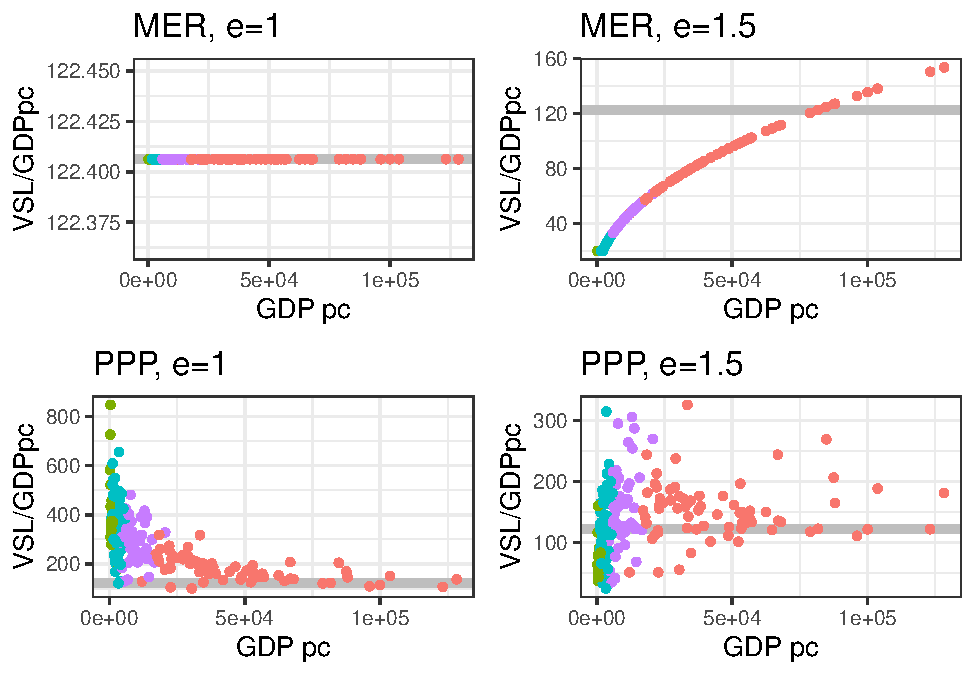
\includegraphics{README_files/figure-latex/pppelasticity-1.pdf}
\caption{\label{fig:pppelasticity}Exposition of different methods to estimate VSL from GNI per capita relative to the USA. On the y axis is VSL expressed as a percentage of GDP per capita. The grey line indicates the USA. We compare GNI per capita expressed using market exchange rates vs.~purchasing power parity, and an elasticity of 1 vs.~1.5. Data source: World Bank.}
\end{figure}

\subsection{Lost economic activity}\label{lost-economic-activity}

We measure the cost of economic closures in terms of lost gross value added (GVA): the GDP generated by an economic configuration is the maximum GVA (denoted \(y_j\) for each sector \(j\)) multiplied by the respective sector openings, summed over the period (\(\tau\) days). The maximum possible GDP (which is with no closures) is

\[Y_0=\frac{\tau}{365}\sum_{j=1}^{m_S}y_j\]

for \(m_S\) sectors, and we use pre-pandemic GVA to define the maximum possible values.

All economic sectors contribute GVA according to the level they are open for production, except for the education sector which contributes its maximum possible GVA, \(y_{\text{ed}}\). \(x_{j}(t)\) is the proportion of the workforce contributing to economic production in sector \(j\) out of the total workforce \(N_j\) on day \(t\). The workforce can be additionally depleted due to self isolation, sickness, hospitalisation and death, leaving a smaller fraction (\(`\hat{x}_{j}(t)`\)) to contribute to production.

\begin{Shaded}
\begin{Highlighting}[]
\NormalTok{\textbackslash{}hat\{x\}\_\{j\}(t)=x\_\{j\}(t)\textbackslash{}left(1 {-} \textbackslash{}left(p\_j\^{}\{23\}(t)  + (1{-}q\_j)p\_j\^{}\{22\}(t)\textbackslash{}right)/N\_j\textbackslash{}right)}
\end{Highlighting}
\end{Shaded}

where \(q_j\) is the fraction of the sector working from home. \(p_j^{23}(t)\) represents worker sickness and death:

\[p_j^{23}(t)=\sum_{v=0}^{m_V}\left(\left(1-p^H_{j,v}\right)p^1p^{19}I_{j,v}^{s}+p^H_{j,v}p^1I_{j,v}^{s}+H_{j,v}+D_{j,v}\right),\]

with \(m_V=2\) vaccines and \(p_j^{22}(t)\) represents lost output from asymptomatic self-isolating workers:

\[p_j^{22}(t)=p^2(t)p^{18}I_{j}^{a}.\]

\(p^{18}\) is the number of days spent in self isolation per day of infectiousness (e.g.~suppose the average infectious period is four days and mandatory self-isolation time is ten days, then \(p^{19}=2.5\) and \(p^{18}=p^{19}T^{I^s}/T^{I^a:R}\), where \(T^{I^s}\) and \(T^{I^a:R}\) are expected infectious periods for symptomatic and asymptomatic, respectively). \(p^1\) is compliance with the requirement to self isolate and \(p^2(t)\) is the fraction of cases identified. Other notations are vaccine status \(v\), infectious and asymptomatic \(I_{j,v}^{a}\), infectious and symptomatic \(I_{j,v}^{s}\), hospitalised \(H\), deceased \(D\), and probability to be hospitalised \(p^H\).

Then the total GDP is

\begin{Shaded}
\begin{Highlighting}[]
\NormalTok{Y =  \textbackslash{}frac\{1 \}\{365\} \textbackslash{}sum\_\{j\textbackslash{}neq\textbackslash{}text\{ed\}\}\^{}\{m\_S\}y\_j\textbackslash{}int\_\{t=0\}\^{}\{\textbackslash{}tau\}\textbackslash{}hat\{x\}\_\{j\}(t)dt + \textbackslash{}frac\{\textbackslash{}tau \}\{365\}\{y\_\textbackslash{}text\{ed\}\},}
\end{Highlighting}
\end{Shaded}

and the GDP loss compared to the maximum is

\[K_2=Y_0-Y.\]

\subsection{Lost education}\label{lost-education}

The loss due to school closure is

\[K_3 =  \frac{1 }{365} \int_{t=0}^{\tau}\left(p^{14}(t)N_{j_{\text{school}}} + (1-p^{14}(t))p^{25}(t)  +(1-2p^{14}(t))p^{24}(t)\right)dt,\]

where \(p^{14}(t)\) is the effective amount of education lost per student at time \(t\) due to school closure:
\[p^{14}(t) = (1-p^{16})(1-x_{\text{ed}}(t)),\]
\(N_{j_{\text{school}}}\) is the total number of students, \(p^{16}\) is relative effectiveness of remote education and \(x_{\text{ed}}(t)\) is the openness of schools, \(p^{25}(t)\) represents education lost due to student sickness with COVID-19:

\[p^{25}(t)=\sum_{v=0}^{m_V}\left((1-p^H_{j_{\text{school}},v})p^1p^{19}I_{j_{\text{school}},v}^{s}+p^H_{j_{\text{school}},v}p^1I_{j_{\text{school}},v}^{s}+H_{j_{\text{school}},v}\right),\]

\(p^{18}\) is the number of days spent in self isolation per day of infectiousness (e.g.~suppose the average infectious period is four days and mandatory self-isolation time is ten days, then \(p^{19}=2.5\) and \(p^{18}=p^{19}T^{I^s}/T^{I^a:R}\), where \(T^{I^s}\) and \(T^{I^a:R}\) are expected infectious periods for symptomatic and asymptomatic, respectively), and \(p^{24}(t)\) represents education lost due to asymptomatic self isolation (which comes at a cost only when schools are open):

\[p^{24}(t)=p^2(t)p^{18}I_{j_{\text{school}}}^{a}.\]

For the value of a year of education, we use the method of \citep{Psacharopoulos2021a}.

\[\text{VSY} =  p^{12}\cdot p^{13}\cdot p^{15}.\]

\(p^{12}\) is the present value of lost earnings:

\[p^{12} = \frac{1}{N_{j_{\text{school}}}}\sum_{a\in j_{\text{school}}}\tilde{N}_a\left( \frac{1-(1+r)^{-(m_Y+20-a)}}{r} -  \frac{1-(1+r)^{-(20-a)}}{r}\right)\]

for discount rate \(r=0.03\), number \(\tilde{N}_a\) students currently age \(a\), and expected number of years of work \(m_Y=45\). \(p^{13}\) is mean annual earnings, \(p^{15}=0.08\) is the rate of return for one year.

The value \(p^{16}\) represents the effectiveness of remote teaching, which we sample as a standard uniform random variable. We note that no strong predictors of effectiveness of remote teaching have been identified \citep{Patrinos2023}. We assume that losses are linear in duration of school closure, although there is not consensus even on this \citep{Betthauser2023}. Important factors to include in future work might be those relating to parental circumstances including education level, engagement and socio-economic status \citep{Moscoviz2022}. However, these factors might be more pertinent to intra- rather than international modelling.

\section{Epi model}\label{epi-model}

\subsection{Ordinary differential equations}\label{ordinary-differential-equations}

\begin{align}
\frac{dS_{j,v}}{dt} & = \sum_{u=0}^{v-1}k^9S_{j,u}^{c_v} - \left( k_{j,v}^{1}(t) + \sum_{u=v+1}^{{m_V}}k_{j,v}^{10,c_u}(t) \right)S_{j,v} \\
\frac{dS_{j,u}^{c_v}}{dt} & = k_{j,u}^{10,c_v}(t)S_{j,u} -\left( k_{j,u}^{1}(t) + k^9 \right)S_{j,u}^{c_v}  \\
\frac{dE_{j,v}}{dt} & = k_{j,v}^{1}(t)\left(S_{j,v}+\sum_{u=v+1}^2S_{j,v}^{c_u}\right) - (k^2+k^4)E_{j,v} \\
\frac{dI_{j,v}^a}{dt} & = k^2E_{j,v} - k^3I_{j,v}^a \\
\frac{dI_{j,v}^s}{dt} & = k^4E_{j,v} - (k_{j,v}^{5}+k_{j,v}^{6})I_{j,v}^s \\
\frac{dR_{j,v}}{dt} & = k^3I_{j,v}^a + k_{j,v}^{5}I_{j,v}^s + k_{j}^{7}(t) H_{j,v} - \sum_{u=v+1}^{{m_V}}k_{j,v}^{10,c_u}(t)R_{j,v} + \sum_{u=0}^{v-1}k_{u,j}^{10,c_v}(t)R_{j,v-1}\\
\frac{dH_{j,v}}{dt} & = k_{j,v}^{6}I_{j,v}^s - (k_{j}^{7}(t) + k_{j}^{8}(t)) H_{j,v} \\
\frac{dD_{j,v}}{dt} & =  k_{j}^{8}(t) H_{j,v}
\end{align}

\subsection{Disease state transitions}\label{disease-state-transitions}

\begin{figure}
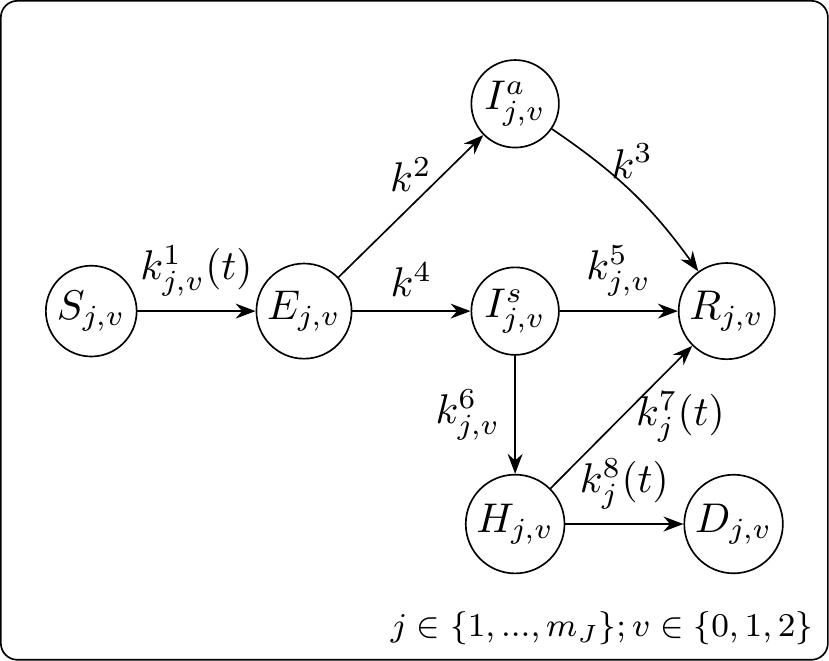
\includegraphics[width=0.5\linewidth]{README_files/figure-latex/statetransitions-1} \caption{Disease state transitions. $S$: susceptible. $E$: exposed. $I^{a}$: asymptomatic infectious. $I^{s}$: symptomatic infectious. $H$: hospitalised. $R$: recovered. $D$: died. $j$: stratum. $v$: vaccination status.}\label{fig:statetransitions}
\end{figure}

Possible transitions between disease states are shown in Figure \ref{fig:statetransitions}. Transition rates are functions of time \(t\), vaccination status \(v\), and group identity \(j\) (where the groups are the 45 sectors and the four age groups).

The rate of infection of susceptible individuals, \(`k^{1}_{j,v}(t)`\), is defined as

\begin{equation}
k_{j,v}^{1}(t) = \eta_{v}^{E}\rho(t)\beta\sum_{h=1}^{m_J}M_{j,h}(x) I_h(t)
\label{eq:infection}
\end{equation}

with \(m_J=49\) strata and

\begin{Shaded}
\begin{Highlighting}[]
\NormalTok{ I\_h(t)=\textbackslash{}sum\_\{v=0\}\^{}\{m\_V\}\textbackslash{}left(\textbackslash{}epsilon (1{-}p\^{}3(t))I\_\{h,v\}\^{}\{a\}(t)+(1{-}p\^{}4(t))I\_\{h,v\}\^{}\{s\}(t)\textbackslash{}right). }
\end{Highlighting}
\end{Shaded}

Here, \(`\eta^{E}_{v}`\) is the relative probability to be infected given vaccine status \(v\); \(\rho(t)\) is the time-dependent modifier of the rate of infection, \(\beta\), which captures the impact of uncosted transmission reductions; \(M(x)\) is the contact matrix between groups and depends on the economic configuration \(x\); \(\epsilon\) is the reduction in infectiousness from asymptomatic relative to symptomatic individuals; \(p^3\) and \(p^4\) are the proportions of asymptomatic and symptomatic infectiousness averted, respectively, due to self isolating; and \(I_{h,\cdot}^{\cdot}\) is the number of infectious asymptomatic (\(I_{h,\cdot}^{a}\)) and symptomatic (\(I_{h,\cdot}^{s}\)) people who are unvaccinated (\(I_{h,v=0}^{\cdot}\)), vaccinated with the BPSV (\(I_{h,v=1}^{\cdot}\)), or vaccinated with the specific vaccine (\(I_{h,v=2}^{\cdot}\)) in stratum \(h\).

\begin{Shaded}
\begin{Highlighting}[]
\NormalTok{ k\^{}2 = \textbackslash{}big(1{-}p\^{}\{I\^{}S\}\textbackslash{}big)/T\^{}\{E:I\} }
\end{Highlighting}
\end{Shaded}

is the rate to asymptomatic infectiousness, where \(p^{I^S}\) is the probability to become symptomatic given infection, and \(T^{E:I}\) is the expected duration of the latent period before the onset of infectiousness;

\begin{Shaded}
\begin{Highlighting}[]
\NormalTok{ k\^{}3 = 1/T\^{}\{I\^{}a:R\}  }
\end{Highlighting}
\end{Shaded}

is the rate of recovery from asymptomatic infection;

\begin{Shaded}
\begin{Highlighting}[]
\NormalTok{ k\^{}4 = p\^{}\{I\^{}S\}/ T\^{}\{E:I\}; }
\end{Highlighting}
\end{Shaded}

is the rate of symptom onset;

\begin{Shaded}
\begin{Highlighting}[]
\NormalTok{k\^{}\{5\}\_\{j,v\} =  \textbackslash{}big(1{-}p\^{}H\_\{j,v\}\textbackslash{}big) / T\_\{j,v\}\^{}\{I\^{}s\}}
\end{Highlighting}
\end{Shaded}

is the rate of recovery from symptomatic infection, where \(p^H_{j,v}\) is the probability to be hospitalised given symptomatic infection, and \(T_{j,v}^{I^s} = p^H_{j,v}T^{I^s:H} + (1-p^H_{j,v})T^{I^s:R}\) is the expected time to be in compartment \(I^s\): \(T^{I^s:H}\) is the expected duration before hospitalisation and \(T^{I^s:R}\) is the expected duration before recovery.

\begin{Shaded}
\begin{Highlighting}[]
\NormalTok{p\^{}H\_\{j,v\}=\textbackslash{}eta\^{}\{H\}\_\{v\}\textbackslash{}tilde\{p\}\^{}\{H\}\_\{j\}}
\end{Highlighting}
\end{Shaded}

is the baseline probability to be hospitalised (\(`\tilde{p}^{H}_{j}`\)) adjusted by the vaccine effect protecting against hospitalisation (\(`\eta^{H}_{v}`\)). Then

\begin{Shaded}
\begin{Highlighting}[]
\NormalTok{k\^{}\{6\}\_\{j,v\} = p\^{}H\_\{j,v\}/T\_\{j,v\}\^{}\{I\^{}s\}}
\end{Highlighting}
\end{Shaded}

is the rate of hospitalisation following symptomatic infection.

\begin{Shaded}
\begin{Highlighting}[]
\NormalTok{k\^{}\{7\}\_\{j\}(t) = (1{-}p\^{}\{D\}\_\{j\}(t)) / T\_j\^{}\{H\}(t)}
\end{Highlighting}
\end{Shaded}

is the rate of recovery of hospitalised patients, where \(`p^{D}_{j}(t)=\tilde{p}^{D}_{j}f_H(t)`\) is the baseline probability to die given hospitalisation, adjusted by a factor encoding the increase in fatality rate as hospital occupancy increases:

\begin{Shaded}
\begin{Highlighting}[]
\NormalTok{f\_H(t)=\textbackslash{}max\textbackslash{}\{1,1+1.87(H\_\{\textbackslash{}text\{tot\}\}(t){-}H\_\{\textbackslash{}text\{max\}\})/H\_\{\textbackslash{}text\{max\}\}\textbackslash{}\},}
\end{Highlighting}
\end{Shaded}

\begin{Shaded}
\begin{Highlighting}[]
\NormalTok{H\_\{\textbackslash{}text\{tot\}\}(t) = \textbackslash{}sum\_\{v=0\}\^{}\{m\_V\}\textbackslash{}sum\_\{j=1\}\^{}\{m\_J\} H\_\{j,v\}(t).}
\end{Highlighting}
\end{Shaded}

\[T_j^{H}(t) = p_j^{D}(t)T^{H:D} + (1-p_{j}^{D}(t))T^{H:R}\]

is the expected time to be in compartment \(H\): \(T^{H:D}\) is the expected duration before death and \(T^{H:R}\) is the expected duration before recovery. Finally,

\begin{Shaded}
\begin{Highlighting}[]
\NormalTok{k\^{}\{8\}\_\{j\}(t) = p\^{}\{D\}\_\{j\}(t)/T\_j\^{}\{H\}(t)}
\end{Highlighting}
\end{Shaded}

is the rate of death following hospitalisation.

\subsection{Vaccination state transitions}\label{vaccination-state-transitions}

In our model, \(v=0\) refers to unvaccinated people, \(v=1\) to people who have received a full schedule of BPSV, and \(v=2\) to people who have received a full schedule of the specific vaccine. How we model transitions between vaccination states is shown in Figure \ref{fig:vaccinetransitions}.

\(`k^{10,c_1}_{j,v=0}(t)`\) represents the rates of BPSV vaccination of unvaccinated susceptible and recovered people, and \(`k^{10,c_2}_{j,v=1}(t)`\) represents the rates of vaccinating BPSV-vaccinated susceptible and recovered people. \(`k^{10,c_2}_{j,v=0}(t)`\) represents the rates of vaccinating people directly with the specific vaccine. Put more succinctly, \(`k^{10,c_u}_{j,v}(t)`\) is the rate to go from vaccine state \(v\) to \(u\). \(k^9=1/T^c\) is the rate of seroconversion to vaccine-induced immunity, and \(`k^{12}_{j}(t)=k^{1}_{j,v=0}(t)`\) and \(`k^{19}_{j}(t)=k^{1}_{j,v=1}(t)`\) are the rates of infection of just-vaccinated people, which returns them to the epidemiological pathway of the lower vaccination level.

\begin{figure}
\centering
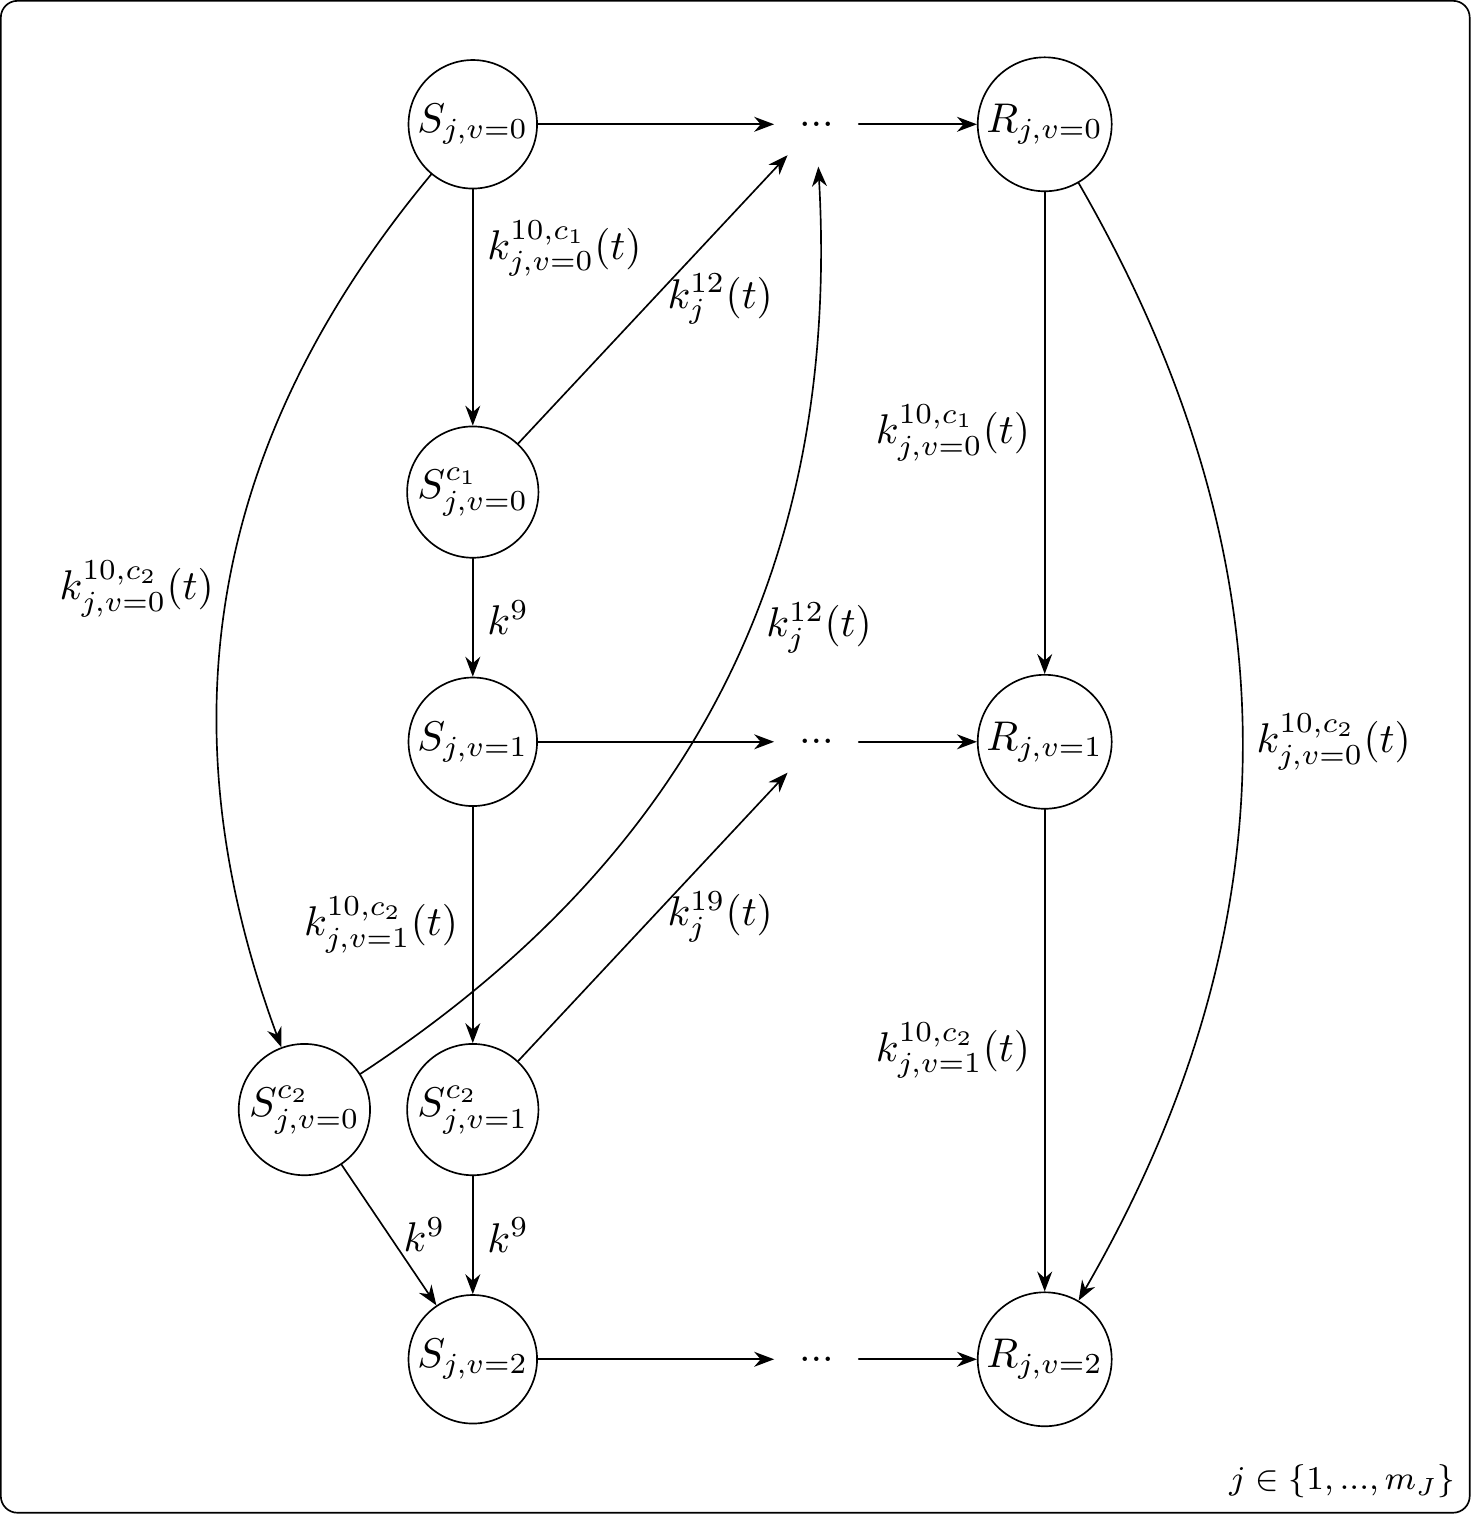
\includegraphics{README_files/figure-latex/vaccinetransitions-1.png}
\caption{\label{fig:vaccinetransitions}Vaccine state transitions. \(S\): susceptible. \(S^{c_u}, u\in\{1,2\}\): recently vaccinated but has not yet seroconverted (i.e.~is not protected by most recent vaccination). \(R\): recovered. \(j\): stratum. \(v\): initial vaccination status. \(u\): final vaccination status.}
\end{figure}

\subsubsection{Vaccine effects}\label{vaccine-effects}

\begin{longtable}[]{@{}lll@{}}
\caption{\label{tab:vaccineeffects} Vaccine effects. The Time to develop immunity is the average time it takes a person to go from the Susceptible compartment to the Vaccinated equivalent compartment, such that the rate of transition 1/21 per day. The Effectiveness against transmission is one minus the relative risk of infection of a vaccinated person compared to an unvaccinated person. The Effectiveness against hospitalisation is one minus the relative risk of hospitalisation of a vaccinated person compared to an unvaccinated person. The Effect on transmission is one minus the relative infectiousness of an infectious vaccinated person compared to an infectious unvaccinated person. The Rate of waning is the rate at which the vaccine effects decay over time.}\tabularnewline
\toprule\noalign{}
Quantity & BPSV & SSV \\
\midrule\noalign{}
\endfirsthead
\toprule\noalign{}
Quantity & BPSV & SSV \\
\midrule\noalign{}
\endhead
\bottomrule\noalign{}
\endlastfoot
Time to develop immunity & 21 days & 21 days \\
Effectiveness against infection & 0.35 & 0.55 \\
Effectiveness against hospitalisation & 0.8 & 0.9 \\
Effect on transmission & 0 & 0 \\
Rate of waning & 0 & 0 \\
\end{longtable}

\subsection{Contact rates}\label{contact-rates}

The configuration \(x\) and the proportion of workers working from home \(q\) determine the scaling of exposure to infection between different groups for different reasons:

\begin{itemize}
\tightlist
\item
  Worker absence due to sector closure
\item
  Worker absence due to working from home
\item
  Student absence due to school closure
\item
  Customer absence due to sector closure: impact on workers
\item
  Customer absence due to sector closure: impact on customers
\end{itemize}

We approach this differently from \citep{Haw2020}. Instead of contact matrices from \citep{Prem2021}, we use those from \citep{Walker2020}. Instead of work contacts from \citep{Beraud2015}, we use those from \citep{Jarvis2023}. \citep{Haw2020} modelled closures using a combination of moving workers between sector compartments and a non-working compartment, and scaling of contacts. Here, we only use contacts to model closures, and do not move workers out of their compartments. An advantage of this is that workers within sectors retain their infection histories.

We construct contact matrix \(M(x)\) as the sum of three matrices: \(M^{\text{com}}(x)\) (community contacts), \(M^{\text{CW}}(x)\) (community-to-worker contacts), and \(M^{\text{WC}}(x)\) (worker-to-community contacts). We construct peacetime matrices (\(x=\textbf{1}\)) beginning with a ``target matrix'', which the three matrices should add up to, which is taken from \citep{Walker2020}. By sampling relevant values, we decompose the whole matrix into its component parts. To incorporate closures, each matrix is transformed independently, before they are all added together again.

Matrix \(M(\textbf{1})\) is estimated using as a basis a contact matrix from \citep{Walker2020}. These are 16-by-16 matrices, \(\tilde{M}\), for five-year age bands \(a\) up to age group 75+. We map the matrix to a four-by-four matrix \(\hat{M}\) corresponding to the four age groups \(g\) used in the DAEDALUS model, using population sizes \(\tilde{N}_a\):

\begin{Shaded}
\begin{Highlighting}[]
\NormalTok{\textbackslash{}hat\{M\}\_\{gg\textquotesingle{}\} = \textbackslash{}frac\{\textbackslash{}sum\_\{a\textbackslash{}in g\}\textbackslash{}tilde\{N\}\_\{a\}\textbackslash{}sum\_\{a\textquotesingle{}\textbackslash{}in g\textquotesingle{}\}\textbackslash{}tilde\{M\}\_\{a,a\textquotesingle{}\}\}\{\textbackslash{}sum\_\{a\textbackslash{}in g\}\textbackslash{}tilde\{N\}\_\{a\}\},}
\end{Highlighting}
\end{Shaded}

and \(\hat{N}_g\) to represent the population sizes of the DAEDALUS age groups,

\begin{Shaded}
\begin{Highlighting}[]
\NormalTok{\textbackslash{}hat\{N\}\_g=\textbackslash{}sum\_\{a\textbackslash{}in g\}\textbackslash{}tilde\{N\}\_a.}
\end{Highlighting}
\end{Shaded}

We get to the matrix \(M(\textbf{1})\) by broadcasting the four-by-four matrix to the 49-by-49 one. Contacts from all groups \(j\) to working groups \(h\) depend on the age group of the group (\(`g(j)`\)), and the fraction of the age-population represented in group \(h\), where \(N_{h}\) is the number of people in group \(h\):

\begin{Shaded}
\begin{Highlighting}[]
\NormalTok{M\_\{j,h\}(\textbackslash{}textbf\{1\}) = \textbackslash{}hat\{M\}\_\{g(j),g(h)\}\textbackslash{}frac\{N\_\{h\}\}\{\textbackslash{}hat\{N\}\_\{g(h)\}\}}
\end{Highlighting}
\end{Shaded}

for \(j\) and \(h\) including all groups (working and non-working). Each group \(j\) contains people that belong to only one age group \(g\). We refer to the age group of the people in group \(j\) as \(g(j)\). Then \(\hat{N}_{g(h)}\) is the number of people in the age group of group \(h\), so \(`\hat{N}_{g(h)}=N_{h}`\) for age groups 0 to 4, 5 to 19 and 65+, and \(`\hat{N}_{g(h)}=\sum_{h\in\{1,...,m_S,m_S+3\}}N_{h}`\) for age group 20 to 64.

In setting up a country, we sample values for \(\tilde{M}\) (from which we get \(`M(\textbf{1})`\)). At the same time, we sample the proportion of contacts that come from workplaces (Figure \ref{fig:workfrac}), and workplace-related contacts. From these, we get \(M^{\text{CW}}(\textbf{1})\), constructing the matrices and normalising.

Community-to-worker contacts (matrix \(M^{\text{CW}}\)) describe contacts experienced by workers from the community by sector (Figure \ref{fig:allsector}, distributed by age, Figure \ref{fig:uksecdistage}). Note that \(`M^{\text{CW}}_{j,h}(\textbf{1})=0`\) for \(j>m_S\). Matrix \(M^{\text{WC}}(\textbf{1})\) is the complement of matrix \(M^{\text{CW}}(\textbf{1})\), computed by multiplying through by population, transposing, and dividing again by population.

With \(M(\textbf{1})\), \(M^{\text{CW}}(\textbf{1})\) and \(M^{\text{WC}}(\textbf{1})\), we learn \(M^{\text{com}}(\textbf{1})\).

\(M^{\text{com}}(\textbf{1})\) is decomposed into its constituent parts, representing intra- and inter-household interactions (home), school interactions (sch) and hospitality interactions (CC):

\begin{Shaded}
\begin{Highlighting}[]
\NormalTok{M\^{}\{\textbackslash{}text\{com\}\}(\textbackslash{}textbf\{1\})=M\^{}\{\textbackslash{}text\{home\}\} + M\^{}\{\textbackslash{}text\{sch\}\}(\textbackslash{}textbf\{1\}) + M\^{}\{\textbackslash{}text\{CC\}\}(\textbackslash{}textbf\{1\}) }
\end{Highlighting}
\end{Shaded}

Values for \(M^{\text{sch}}(\textbf{1})\) come from sampled values representing the fractions of contacts that come from school. School contacts are estimated separately in two age groups (pre-school age: 0-\/--4 (Figure \ref{fig:school1frac}); school age: 5-\/--19 (Figure \ref{fig:school2frac})): \(M^{\text{sch}}(\textbf{1})\) has entries of zero for groups not in school, and values for 0 to 4 year olds and 5 to 19 year olds.

Finally, \(M^{\text{CC}}(\textbf{1})\) is sampled as a fraction of \(M^{\text{com}}(\textbf{1})- M^{\text{sch}}(\textbf{1})\) (Figure \ref{fig:hospfrac}, distributed by age, Figure \ref{fig:conagefrac}), which leaves \(M^{\text{home}}\). Community contacts in consumption settings includes contacts made on public transport, as these contacts are small in number and are most correlated with consumption (and not work or school) \citep{Jarvis2023}. (This might be because contacts are counted by how many people you talk to.)

\begin{figure}
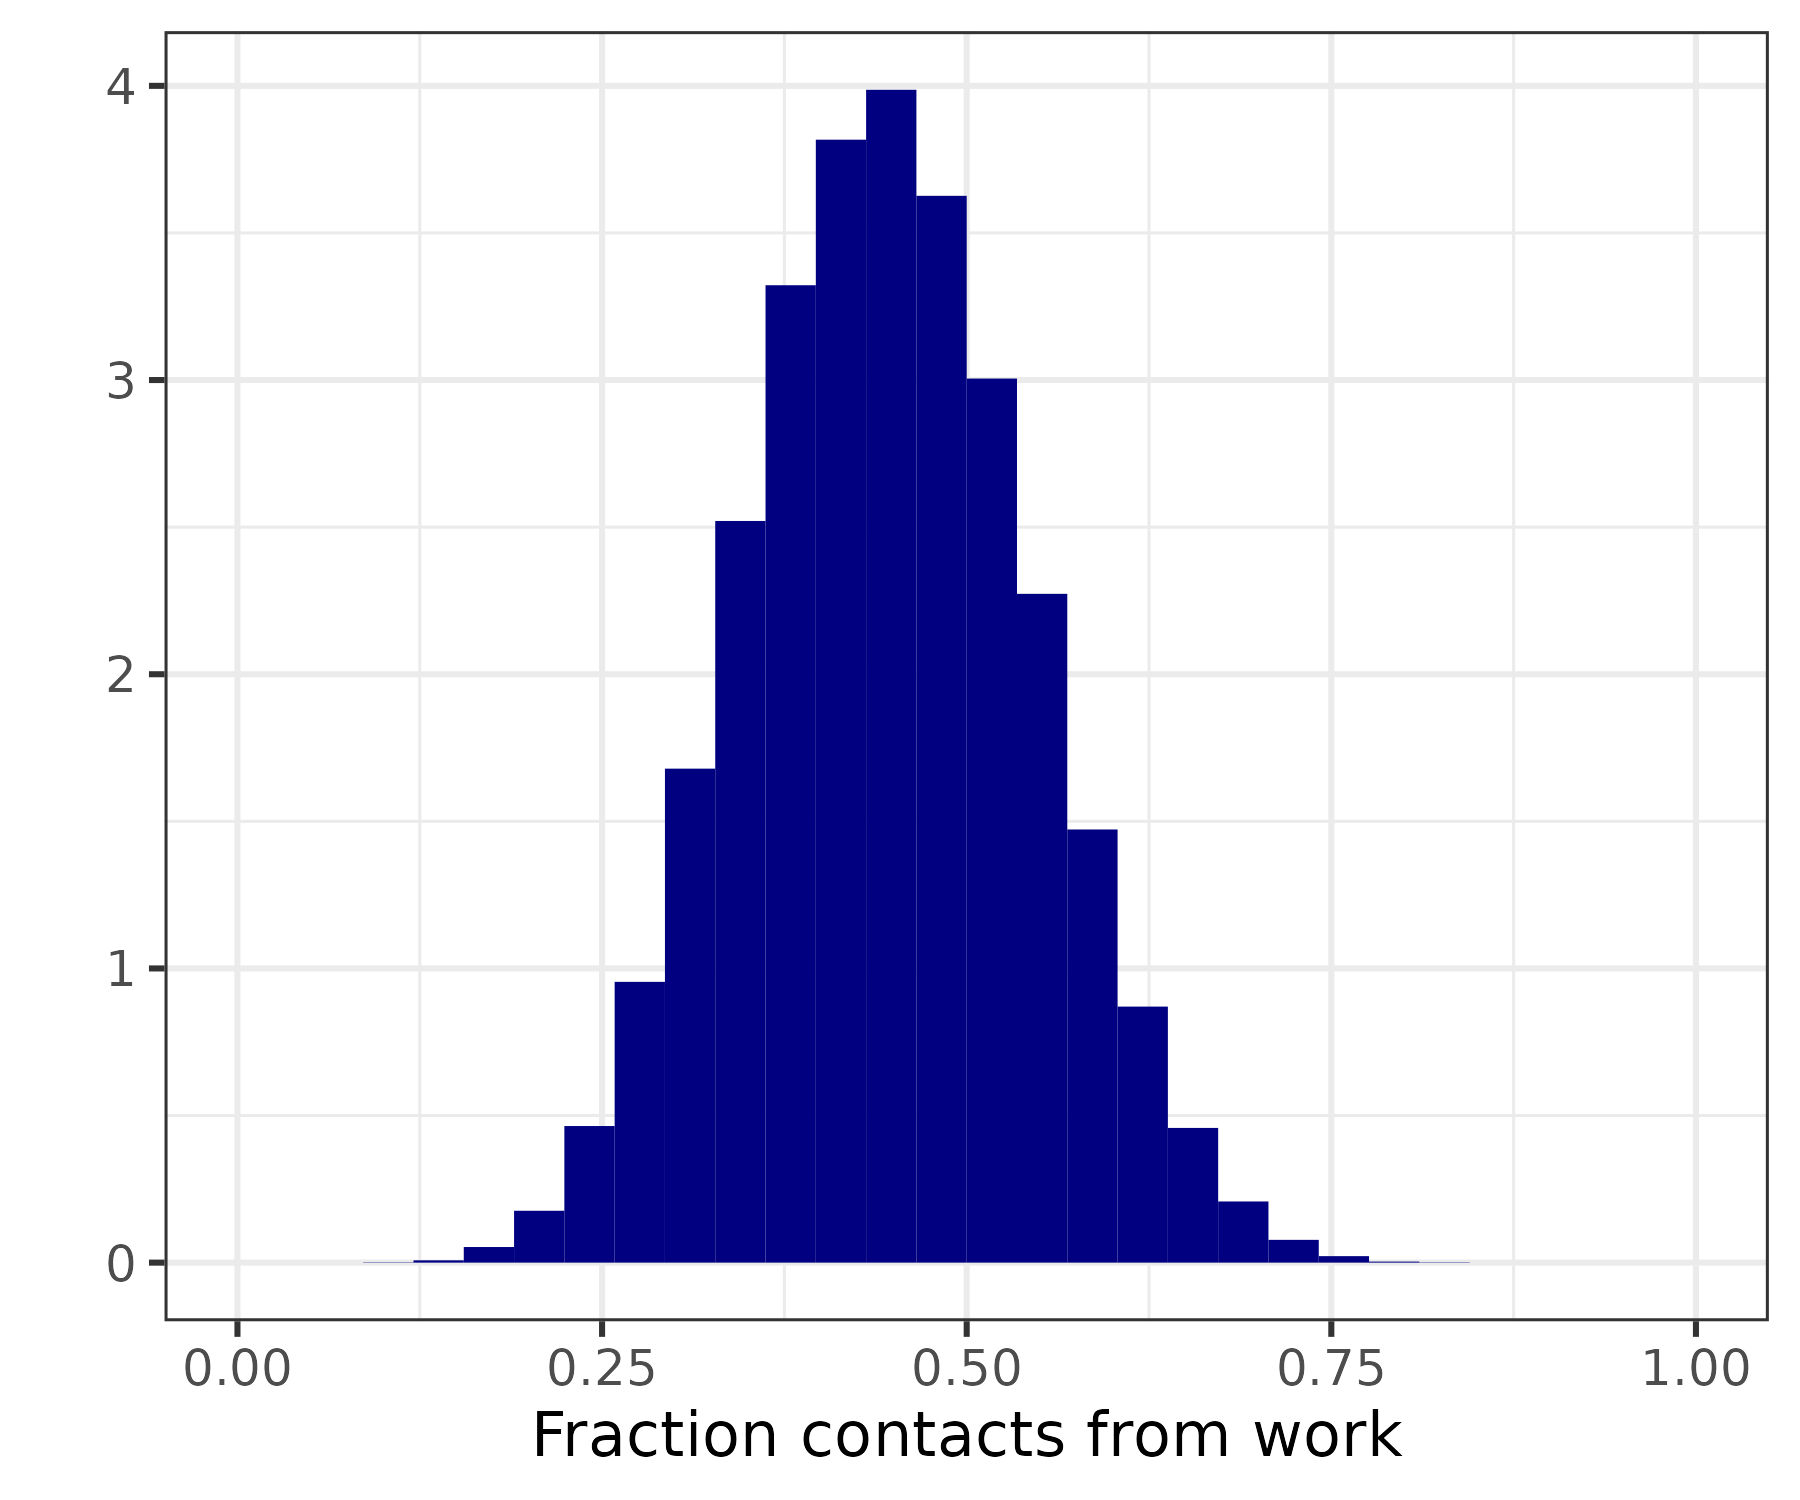
\includegraphics[width=0.5\linewidth]{README_files/figure-gfm/workfrac} \caption{Fraction of contacts made at work, from [@Jarvis2023]. Extrapolated from three countries (UK, Belgium, Netherlands), whose values are all close to 40\%, using time-use survey results for fraction of time spent at work (OECD, last updated December 2023, 33 countries, with values ranging from 12 to 25\% (and the three reference countries have values 16 to 18\%)).}\label{fig:workfrac}
\end{figure}

\begin{figure}
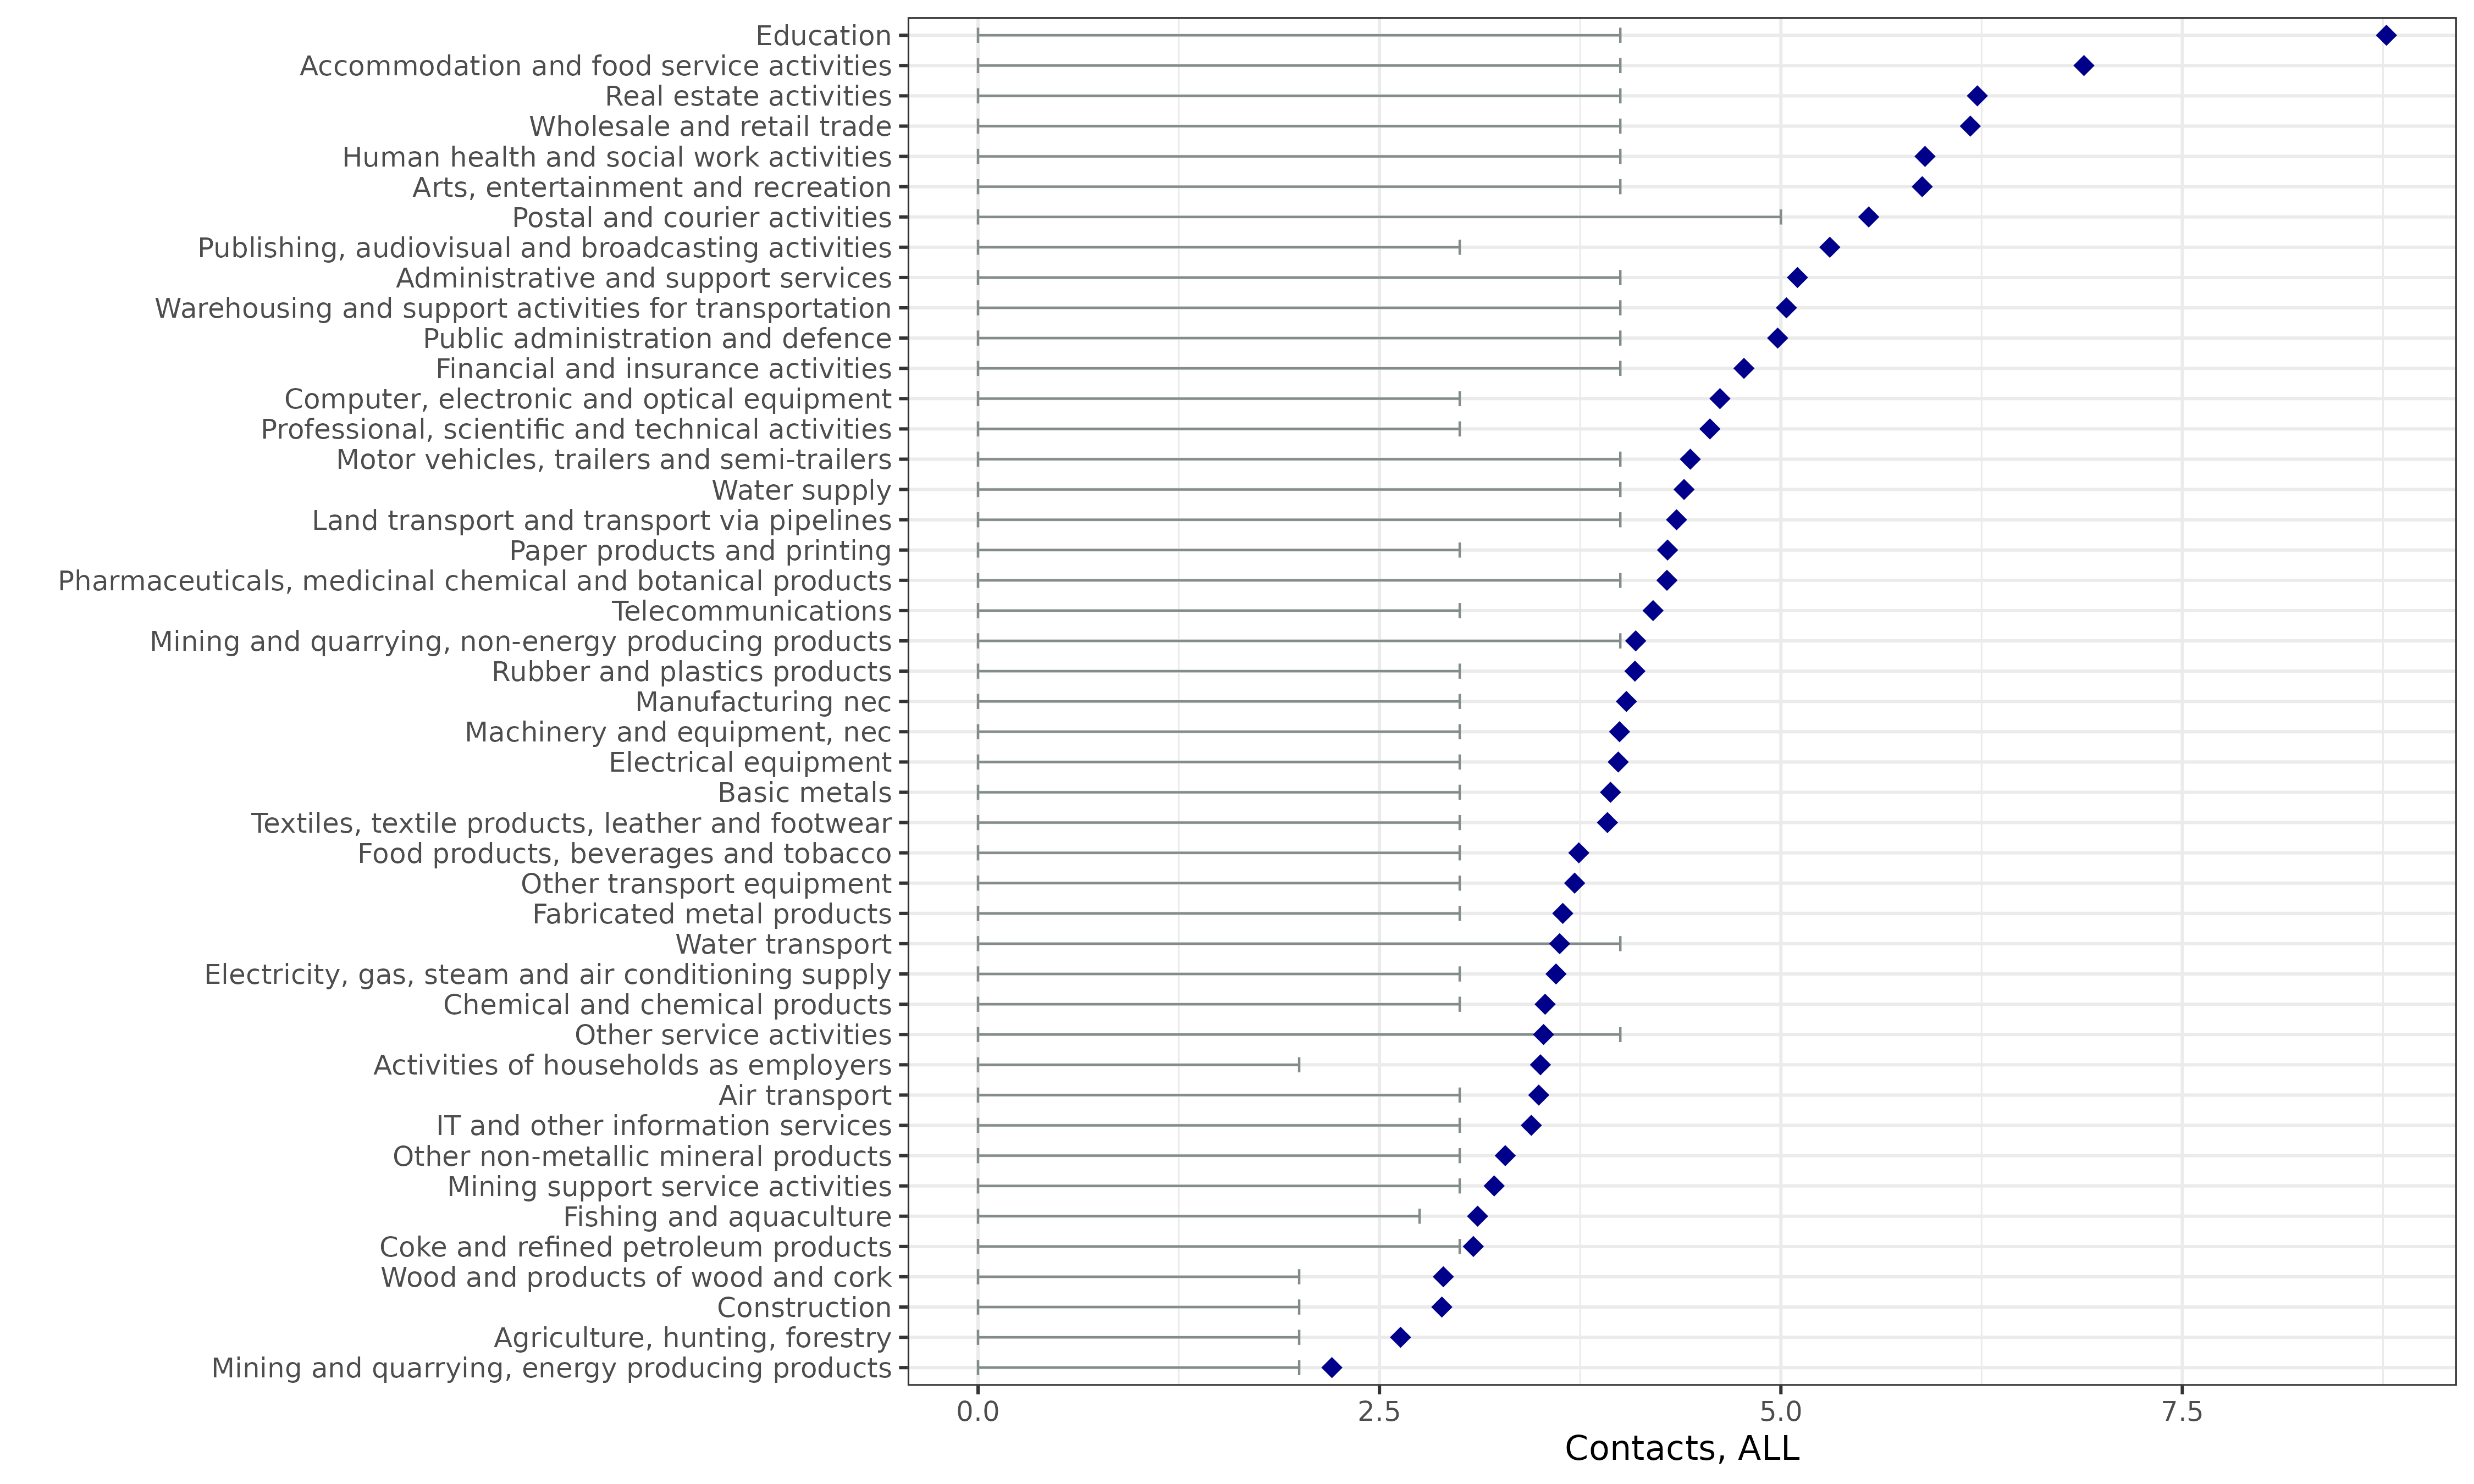
\includegraphics[width=0.5\linewidth]{README_files/figure-gfm/allsector45} \caption{Number of contacts made at work, from [@Jarvis2023]. Diamonds show average numbers and ranges are 50\% quantile intervals. We sample values from half to double the average. Data come from UK, Netherlands and Switzerland, with occupation ISCO-88 mapped to ISCO-08 then SOC-10 then ISIC rev 4 using ONS data.}\label{fig:allsector}
\end{figure}

\begin{figure}
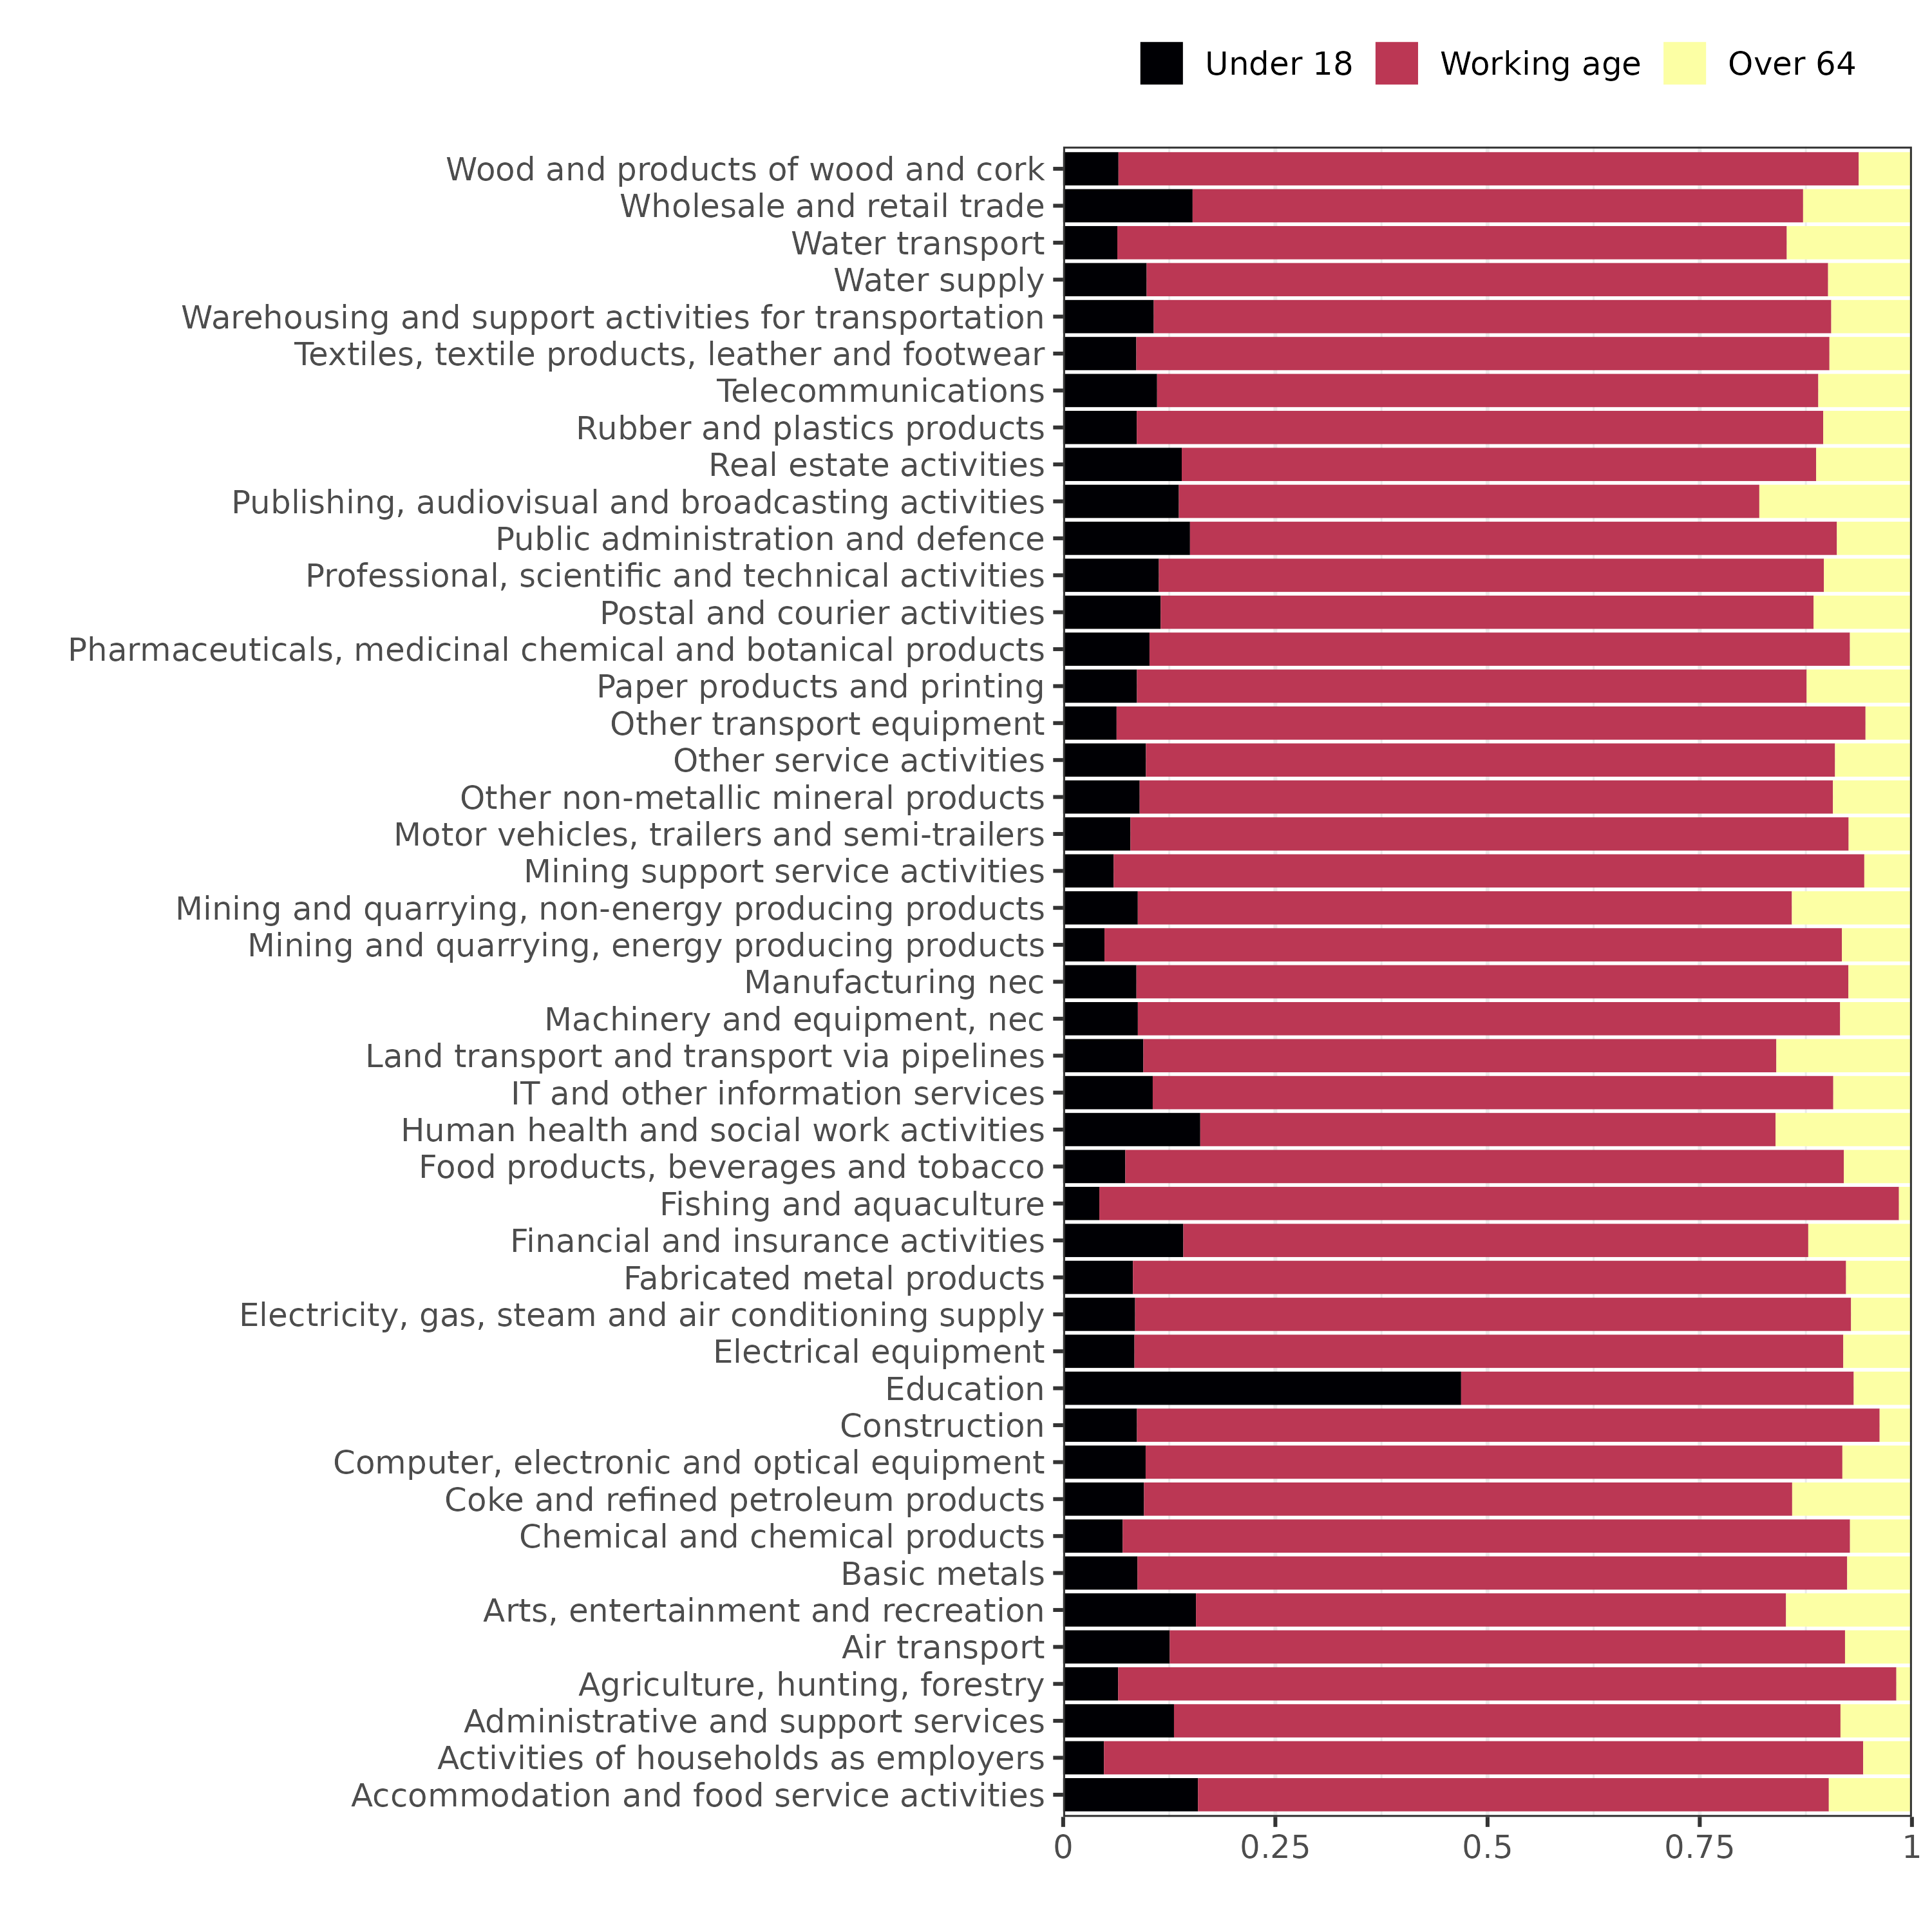
\includegraphics[width=0.5\linewidth]{README_files/figure-gfm/uksec_dist_age} \caption{Fraction of contacts made at work by age, from [@Jarvis2023].}\label{fig:uksecdistage}
\end{figure}

\begin{figure}
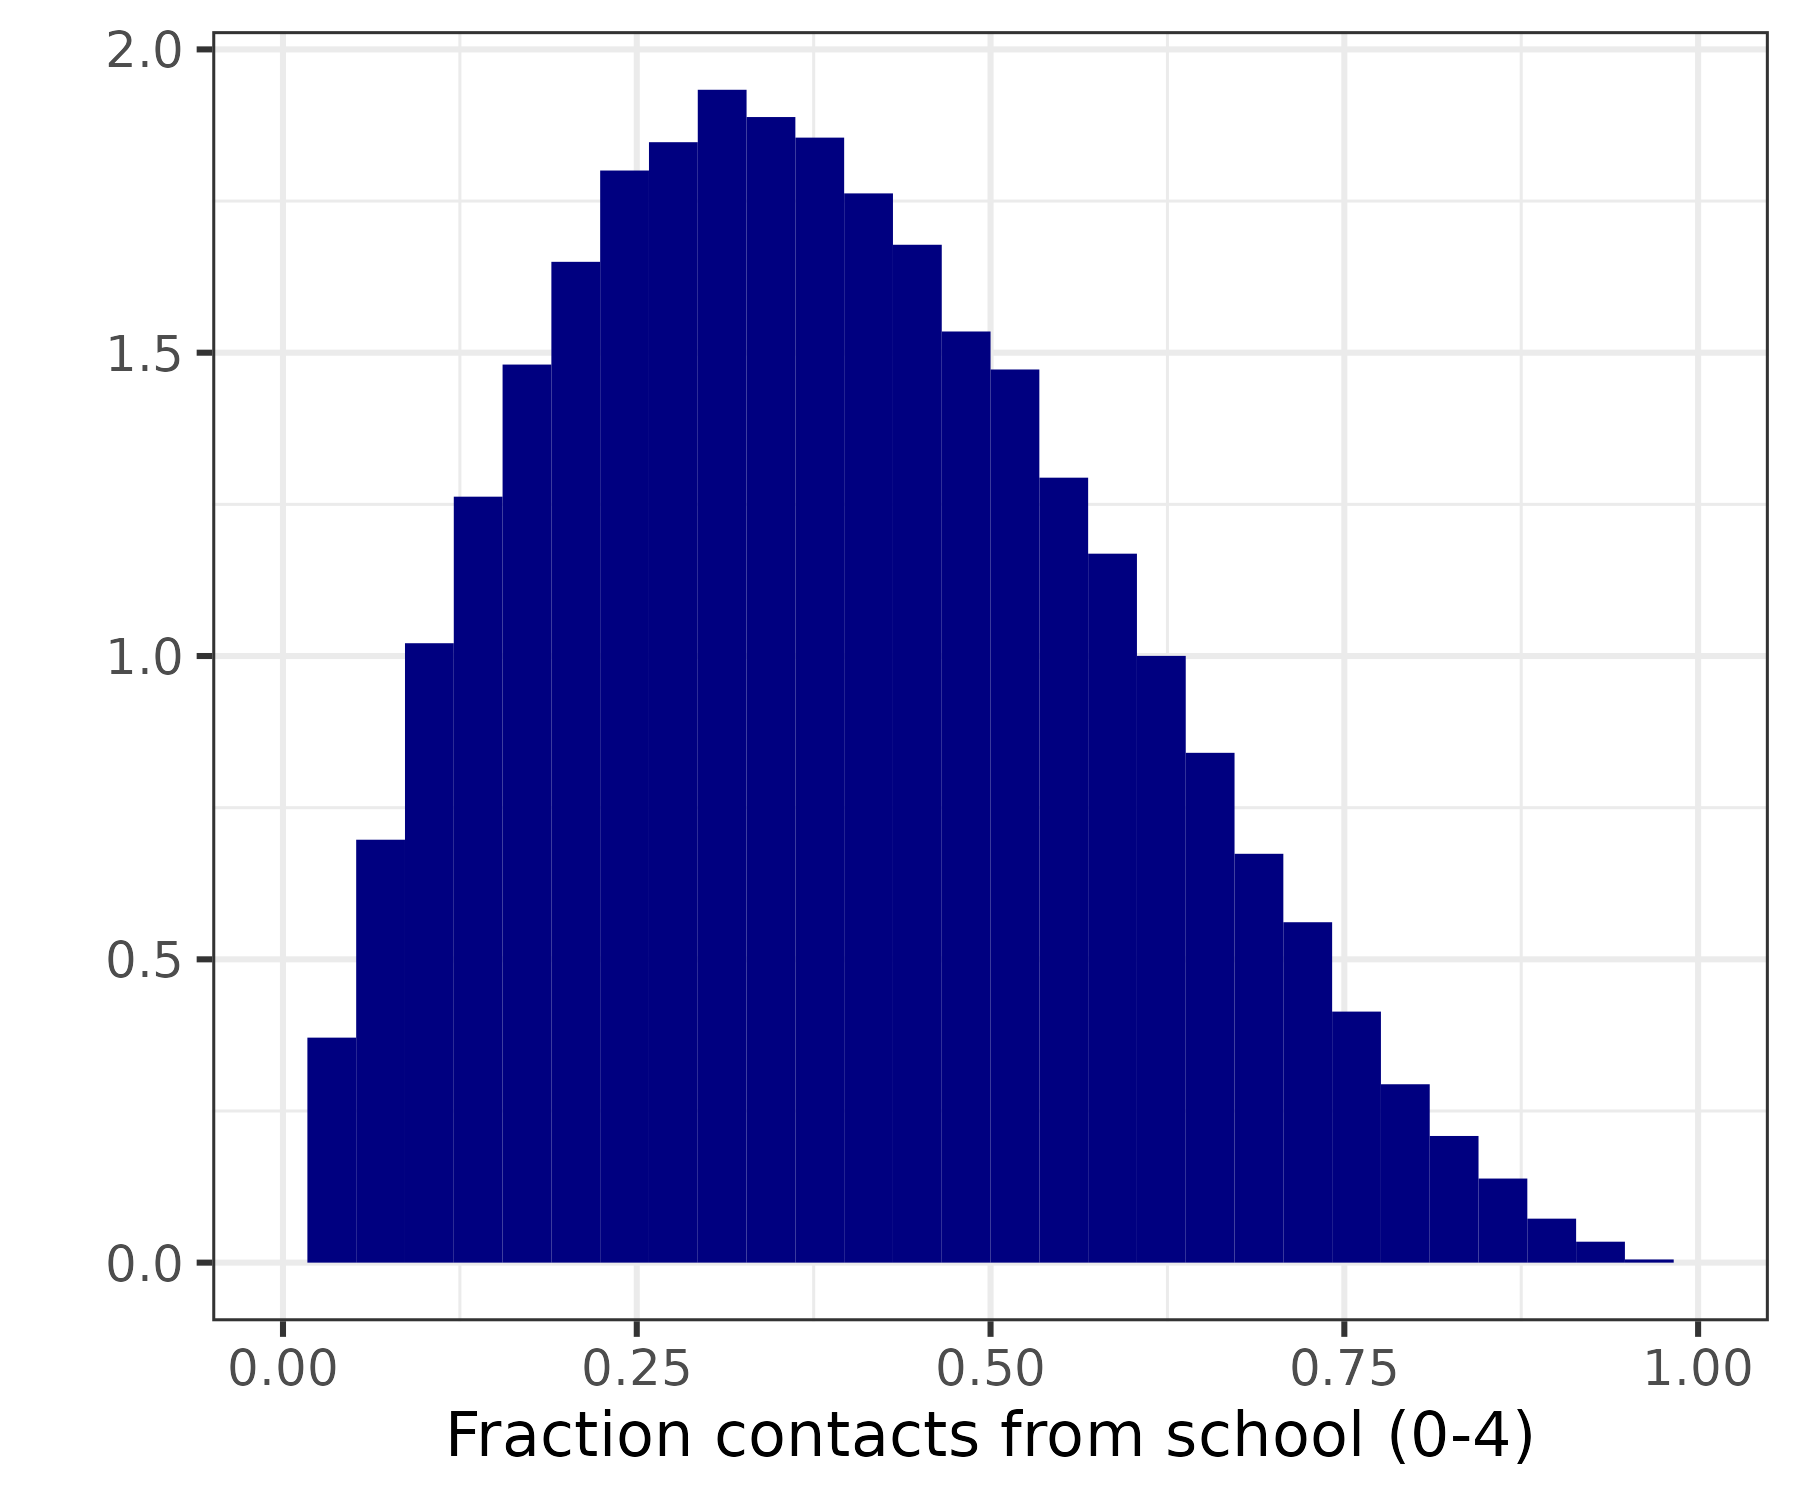
\includegraphics[width=0.5\linewidth]{README_files/figure-gfm/school1frac} \caption{Fraction of contacts made at school for ages 0 to 4, from [@Jarvis2023].}\label{fig:school1frac}
\end{figure}

\begin{figure}
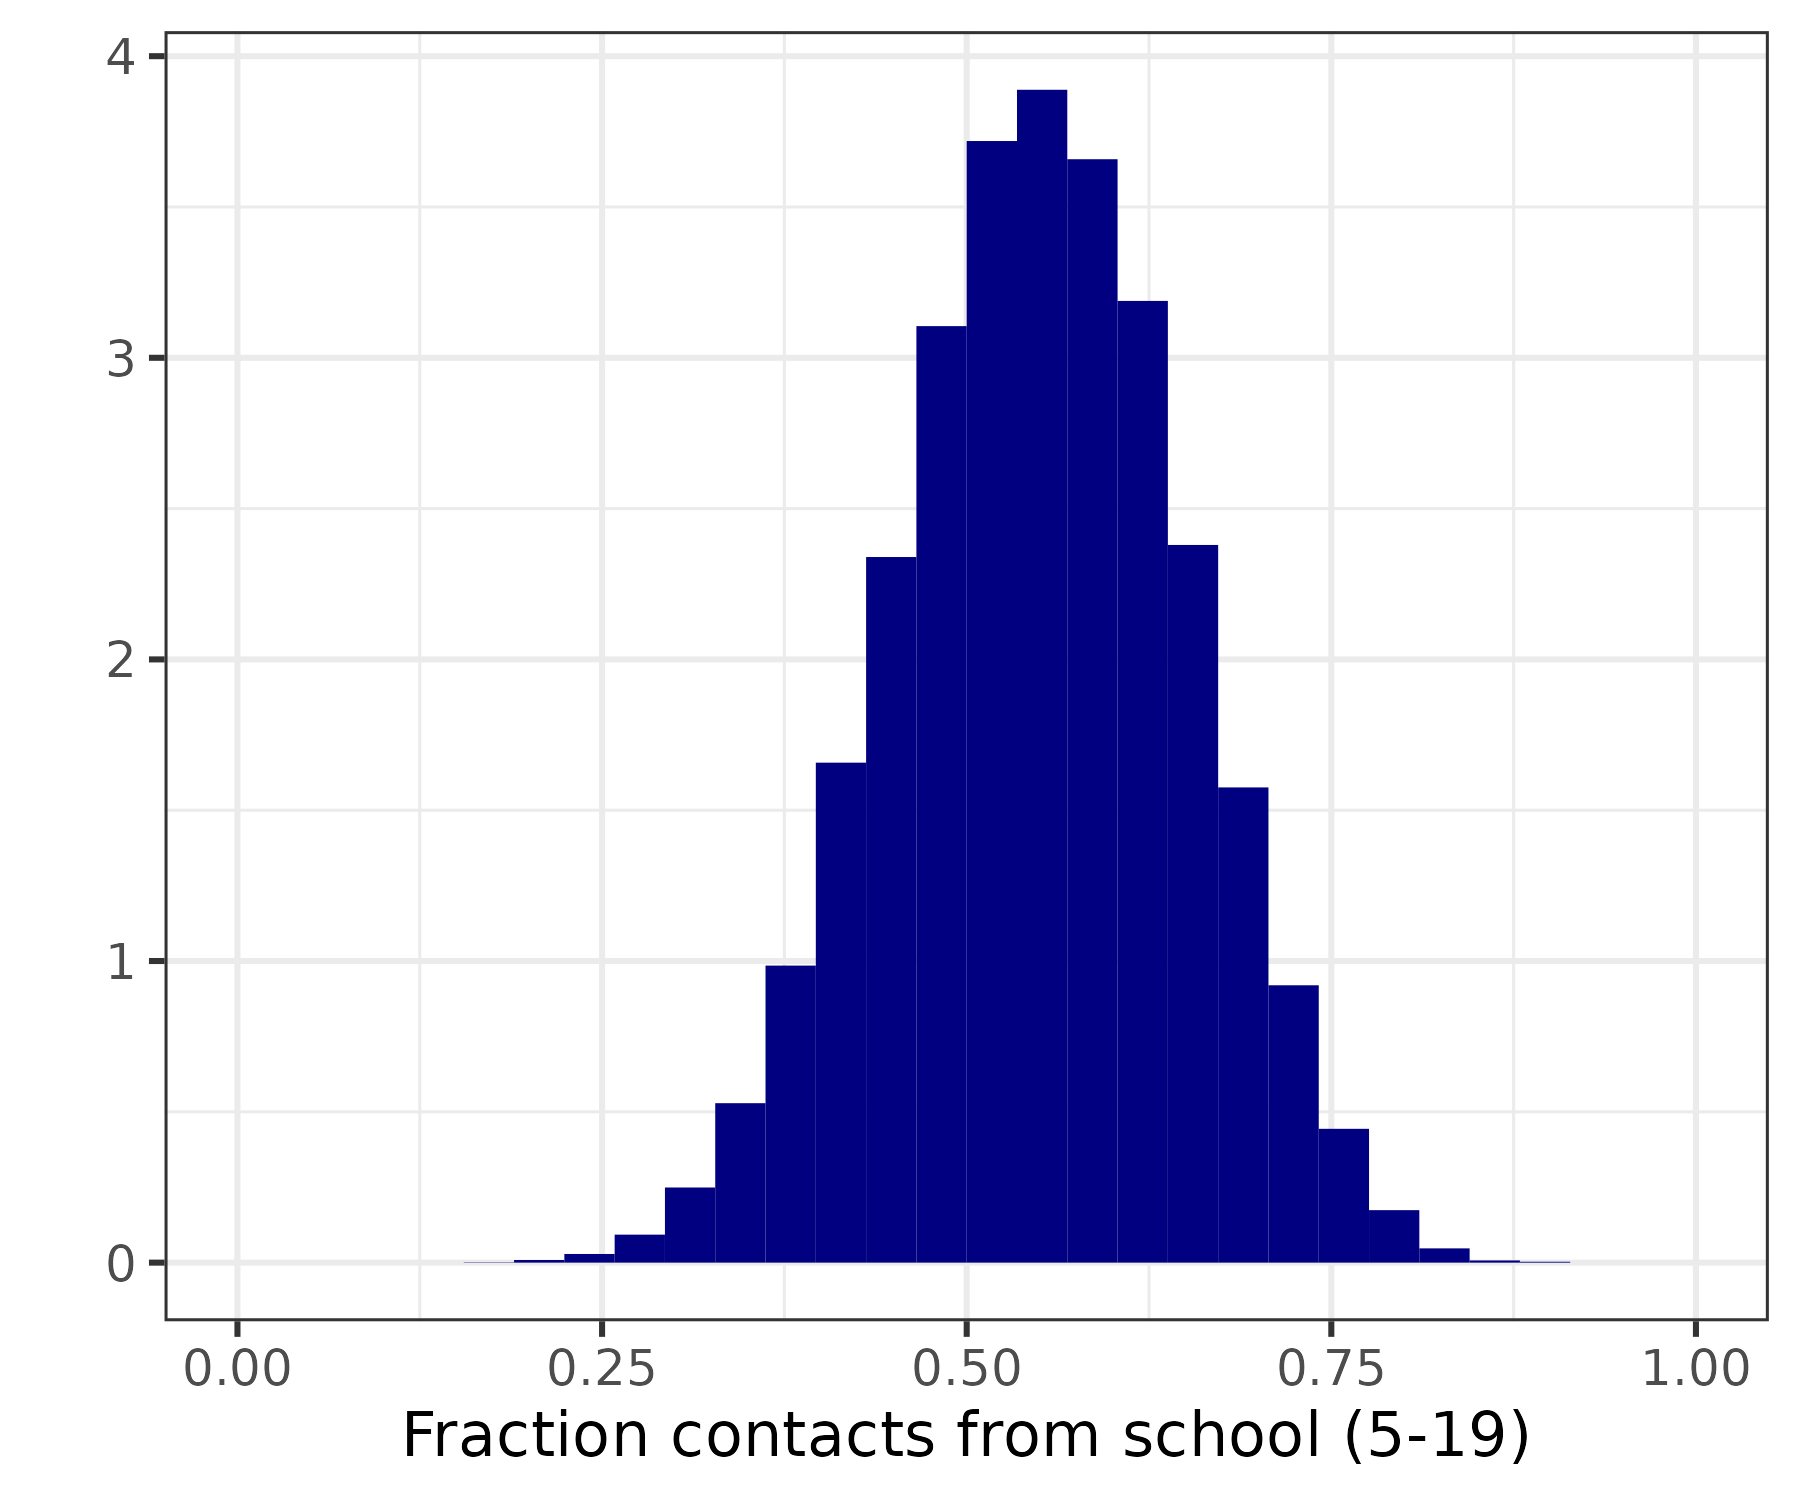
\includegraphics[width=0.5\linewidth]{README_files/figure-gfm/school2frac} \caption{Fraction of contacts made at school for ages 5 to 19, from [@Jarvis2023].}\label{fig:school2frac}
\end{figure}

\begin{figure}
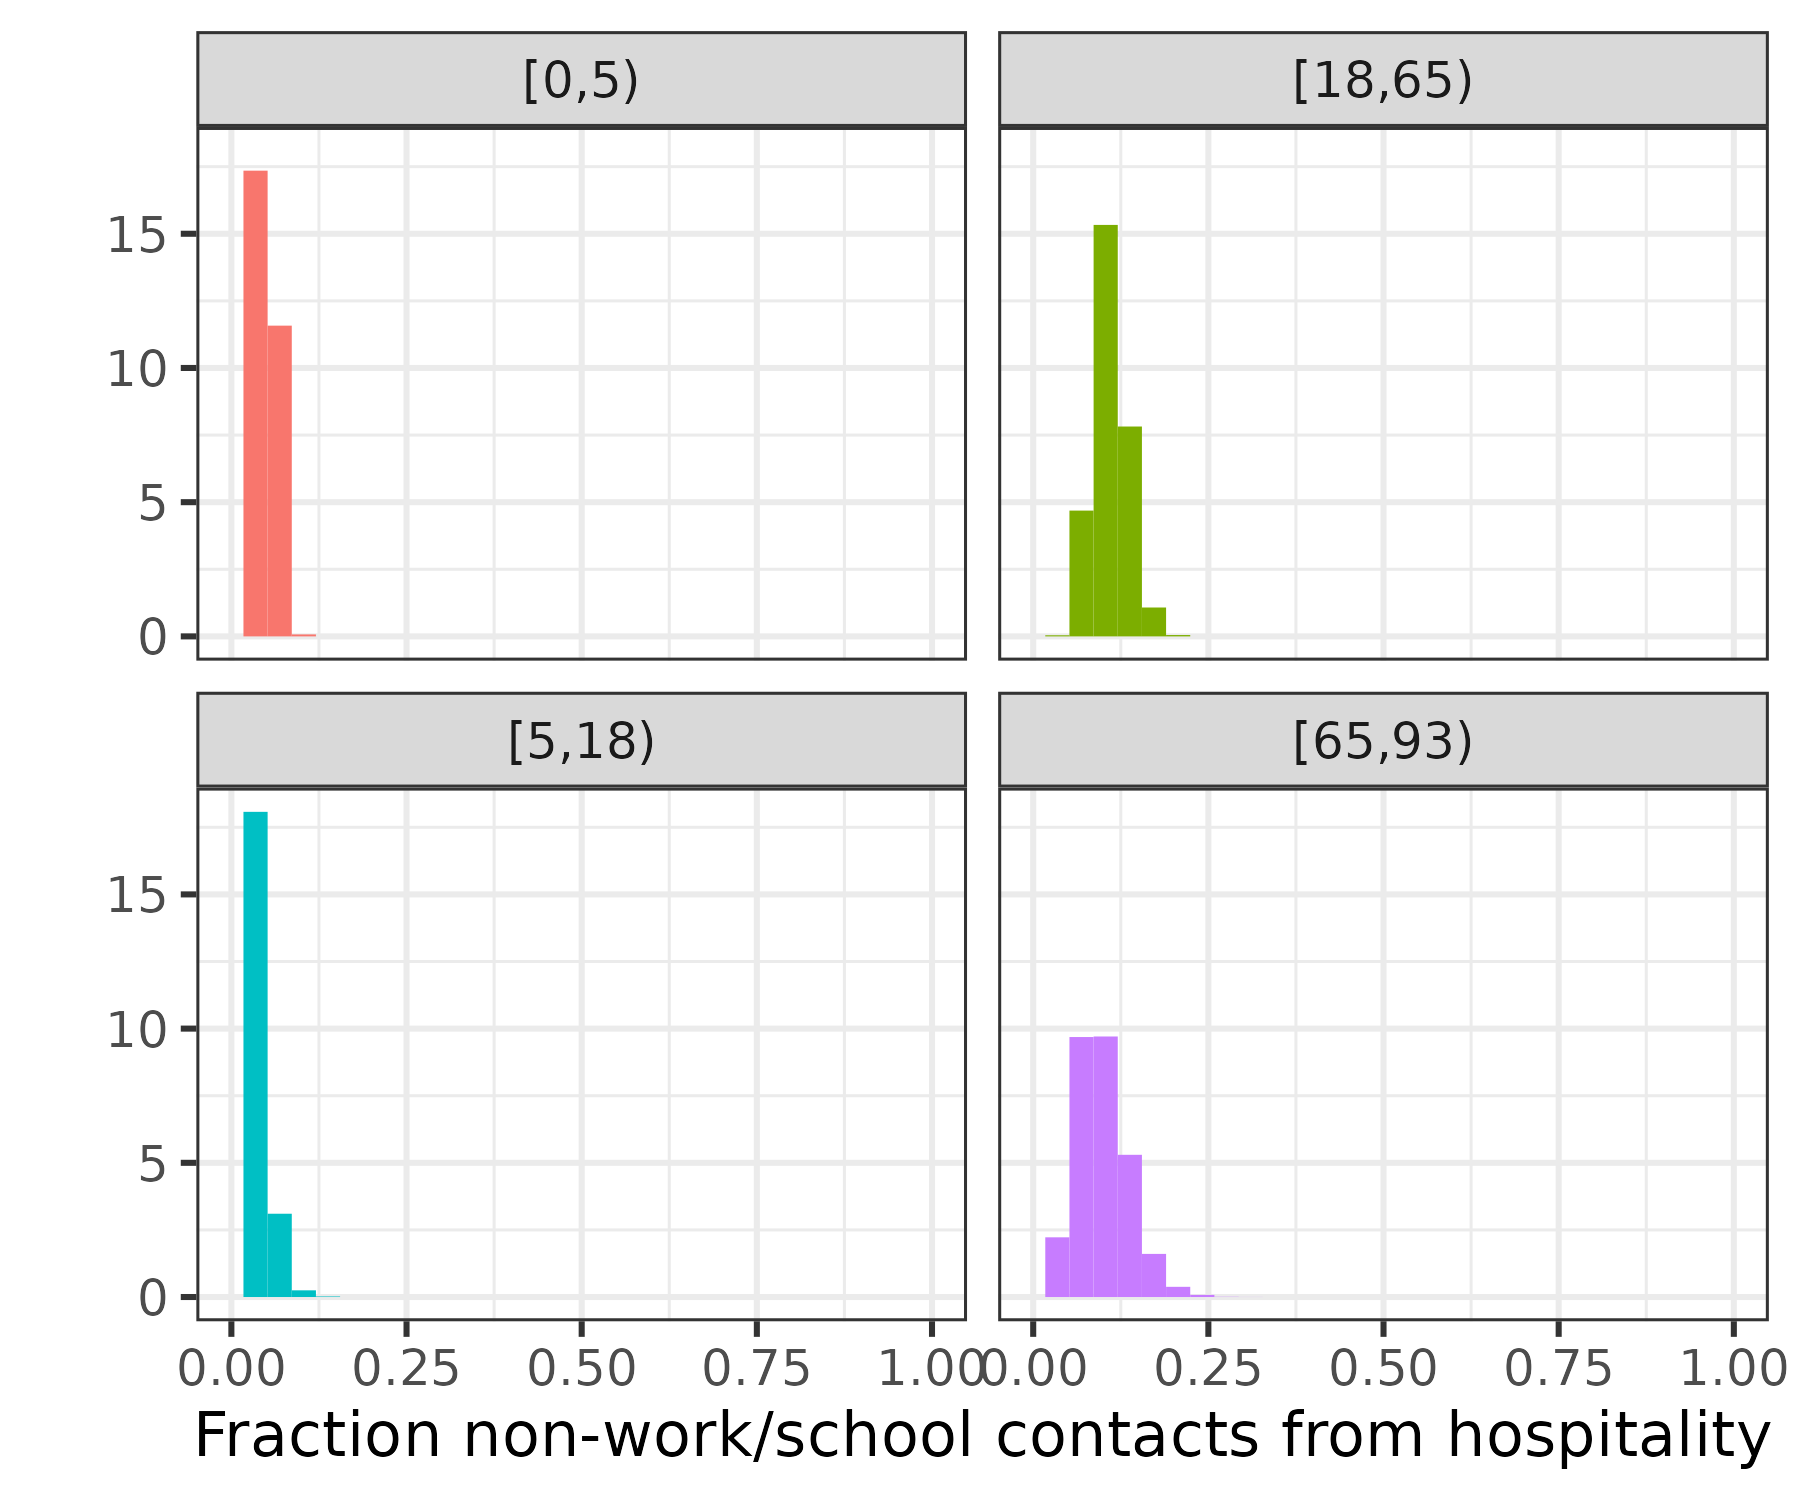
\includegraphics[width=0.5\linewidth]{README_files/figure-gfm/hospfrac} \caption{Fraction of non-school and non-work contacts made in hospitality settings, by age group, from [@Jarvis2023].}\label{fig:hospfrac}
\end{figure}

\begin{figure}
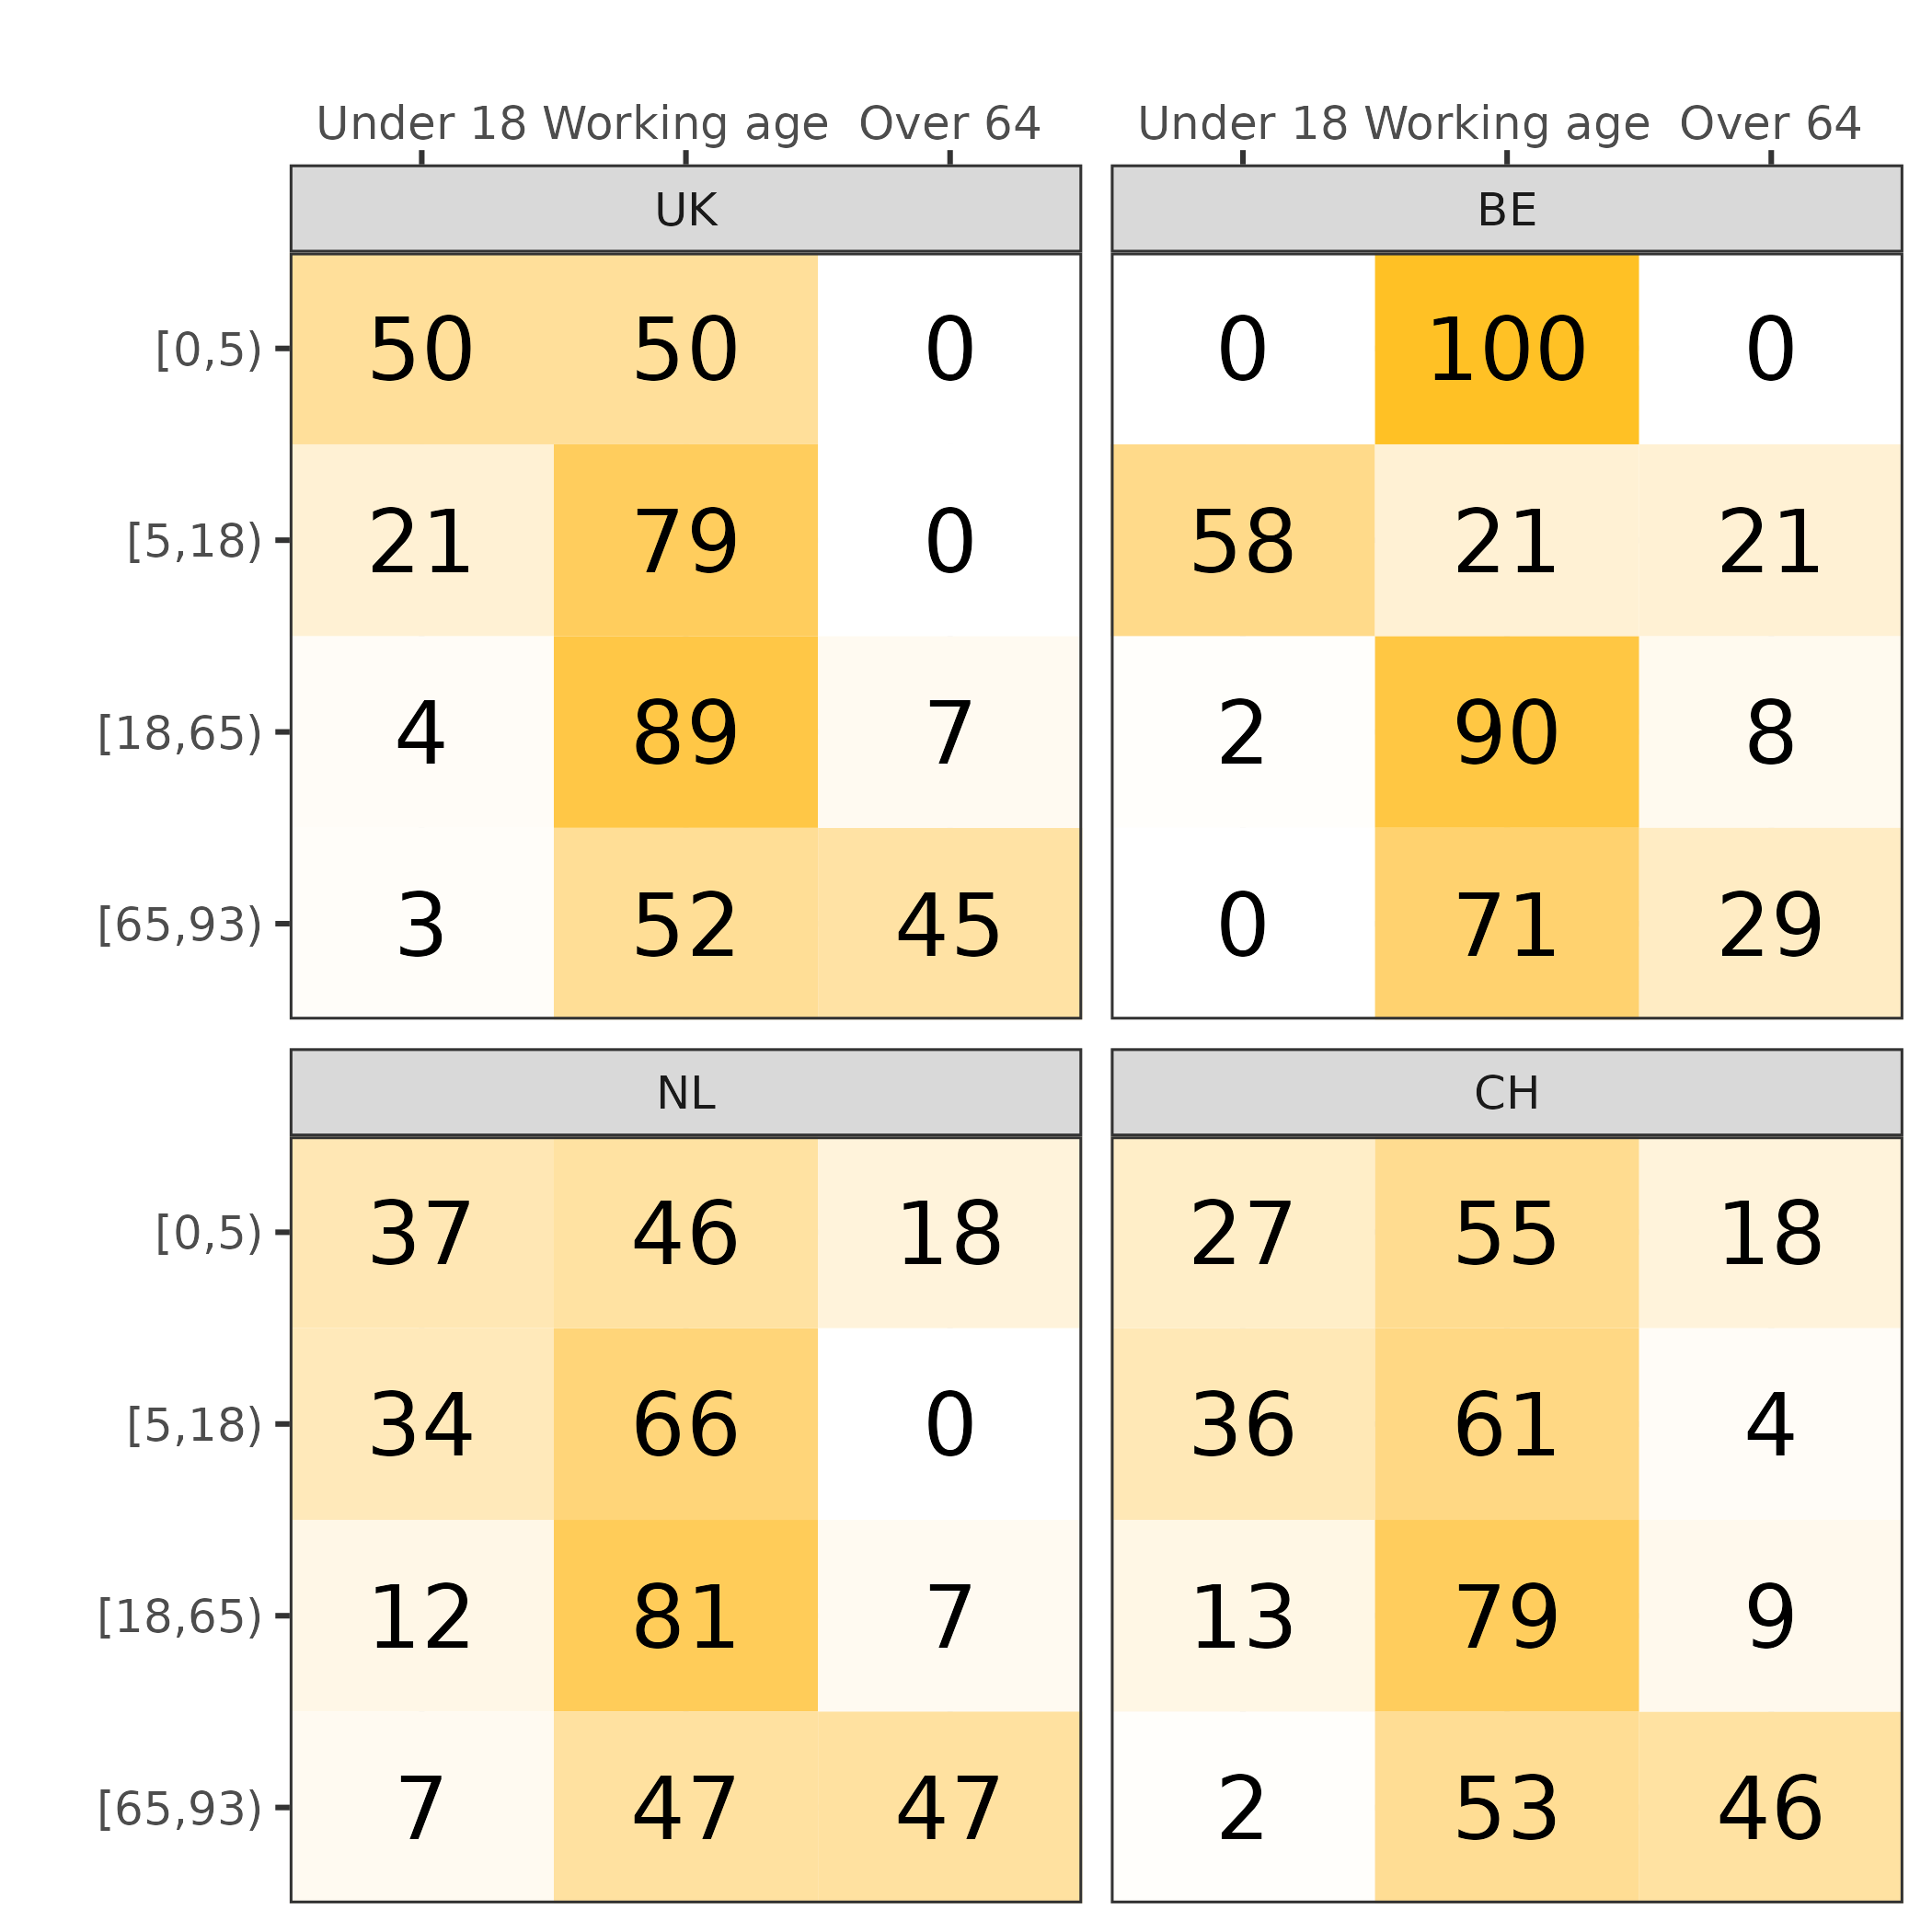
\includegraphics[width=0.5\linewidth]{README_files/figure-gfm/conagefrac} \caption{Distribution of non-school and non-work contacts made in hospitality settings by age group, from [@Jarvis2023].}\label{fig:conagefrac}
\end{figure}

\subsubsection{Community contacts}\label{community-contacts}

We construct \(M^{\text{com}}(x)\) from its constituent parts, representing intra- and inter-household interactions (home), school interactions (sch) and hospitality interactions (CC):

\begin{Shaded}
\begin{Highlighting}[]
\NormalTok{M\^{}\{\textbackslash{}text\{com\}\}(x)=M\^{}\{\textbackslash{}text\{home\}\} + M\^{}\{\textbackslash{}text\{sch\}\}(x) + M\^{}\{\textbackslash{}text\{CC\}\}(x).}
\end{Highlighting}
\end{Shaded}

School contacts under \(x\) are the peacetime values scaled by the extent of closure. \(x_{\text{ed}}\) is the extent to which schools are open, so that the number of contacts per person scales superlinearly with school closure.

\begin{equation}
M_{j,j}^{\text{sch}}(x)=x_{\text{ed}}^2M_{j,j}^{\text{sch}}(\textbf{1}).
\label{eq:school}
\end{equation}

Matrix \(M^{\text{CC}}(x)\) gives the contacts made in the hospitality sector:

\begin{equation}
M^{\text{CC}}(x) = (p^{27})^2M^{\text{CC}}(\textbf{1})
\label{eq:hosp}
\end{equation}

The value \(p^{27}\) is the workforce-weighted average extent to which the hospitality sectors are open, so that the number of contacts per person scales superlinearly according to closure:

\begin{Shaded}
\begin{Highlighting}[]
\NormalTok{p\^{}\{27\} = \textbackslash{}frac\{\textbackslash{}sum\_jx\_\{j\}N\_j\}\{\textbackslash{}sum\_jN\_j\}}
\end{Highlighting}
\end{Shaded}

where we sum over only the hospitality sectors.

\subsubsection{Community-to-worker contacts}\label{community-to-worker-contacts}

\begin{equation}
M_{j,h}^{\text{CW}}(x) = (x_{j}(1-q_j))^2M_{j,h}^{\text{CW}}(\textbf{1}),
\label{eq:ctow}
\end{equation}

for \(h\in\{1,...,m_J\}\).

Here, there is superlinear scaling of \(M^{\text{CW}}_{j,h}(\textbf{1})\) with respect to working from home and with respect to sector closure, as both workers and members of the community are absent from the workplace as the sector moves online and becomes more closed.

\subsection{Uncosted transmission reductions}\label{uncosted-transmission-reductions}

We parametrise the effects of `uncosted transmission reductions' (UTR) in the model using Google's mobility data (Figure \ref{fig:smoothmobility}). These changes in mobility were consequences of both government mandates and individual's choices. As we cannot separate the two, we consider a range of possibilities, based on the range of mobility changes observed for a given level of stringency (Figure \ref{fig:mobilitydrop}). In our model, the mandated economic configuration leads to a change in contacts. We associate the reduction in contacts, which translates as a relative reduction in transmission, with the reduction in mobility.

\begin{figure}
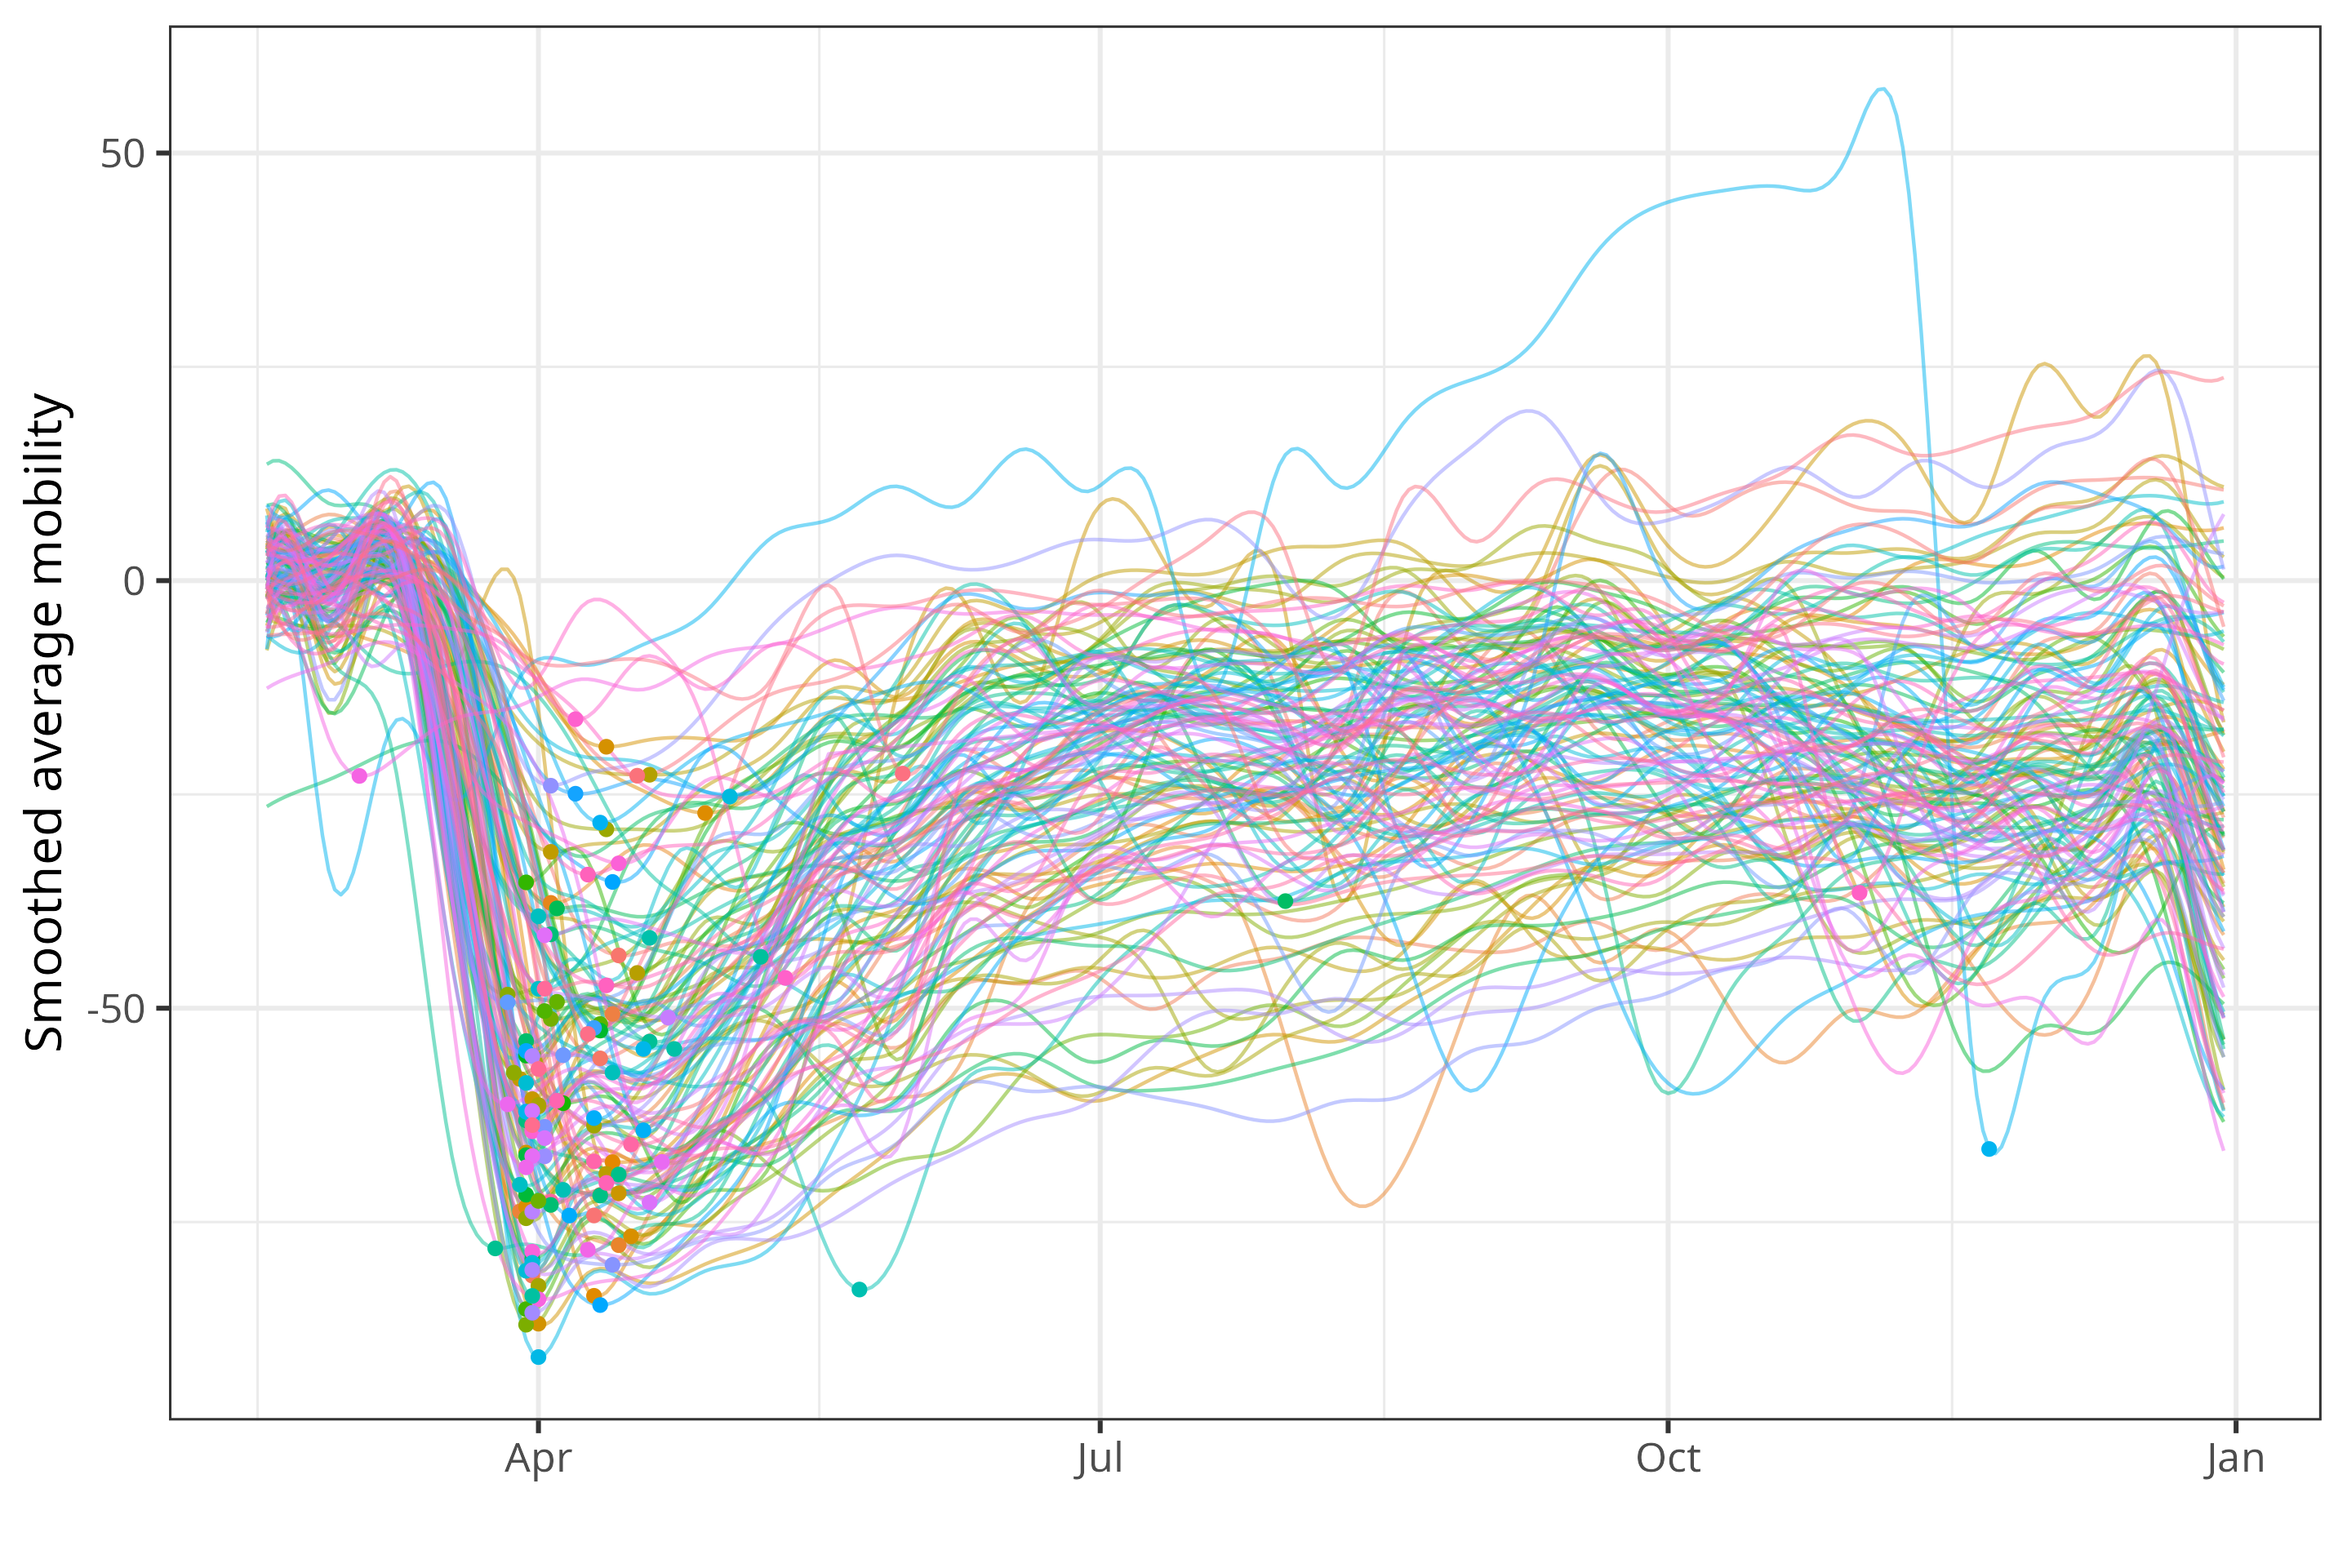
\includegraphics[width=0.5\linewidth]{README_files/figure-gfm/smoothmobility} \caption{Mobility trajectories in 2020 for all countries, with points showing the point at which the largest drop was observed. Trajectories are averaged over "Retail and recreation", "Transit stations" and "Workplaces" and smoothed with a spline of 80 knots.}\label{fig:smoothmobility}
\end{figure}

\begin{figure}
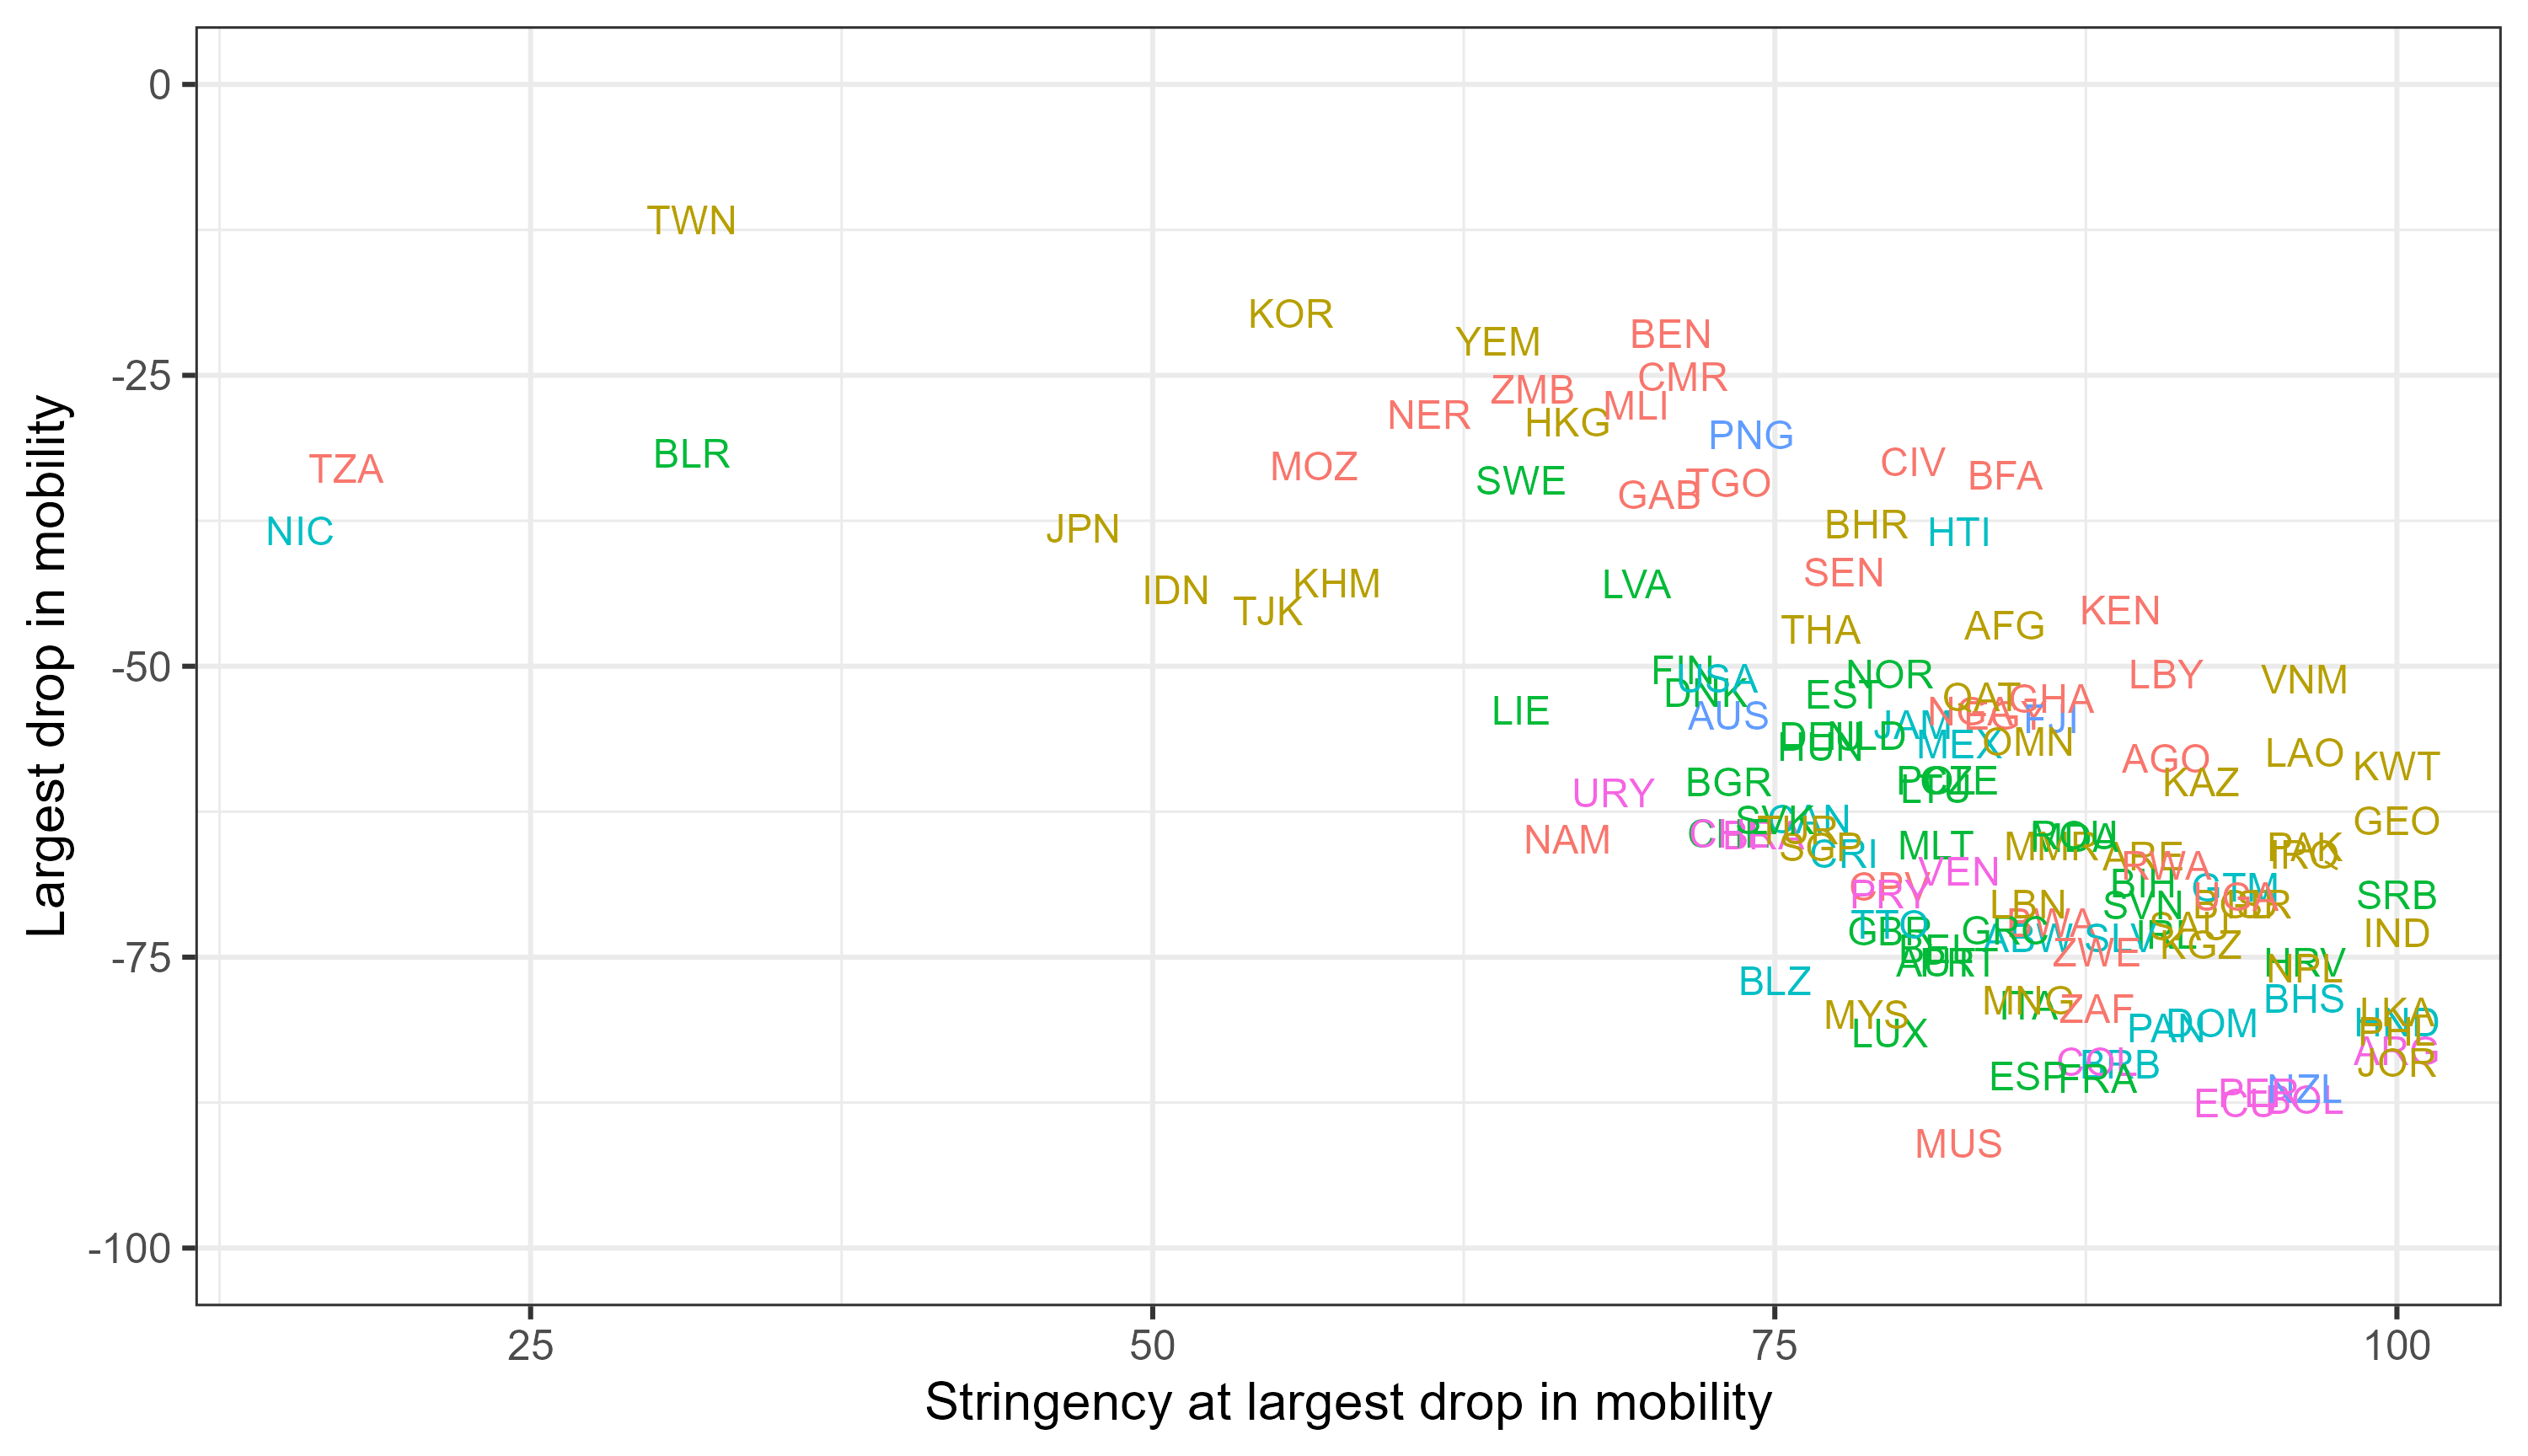
\includegraphics[width=0.5\linewidth]{README_files/figure-gfm/mobilitydrop} \caption{The largest drop in mobility plotted against the stringency on that date.}\label{fig:mobilitydrop}
\end{figure}

\begin{itemize}
\tightlist
\item
  We want to write mobility as a function of mandate and some epi outcome, e.g.~deaths: \(\rho(t) = (1-p^8)f(d(t),e(t)) + p^8\) where \(\rho(t)\) is mobility, \(d\) is deaths per million, \(e\) is government mandate, and \(`0 < p^8 < 1`\) is the baseline.
\item
  We want mobility to drop monotonically with both the mandate and the epi outcome: \(\frac{\partial f}{\partial d}<0\), \(\frac{\partial f}{\partial e}<0\).
\item
  We want a maximum mobility of 1 when both the mandate and the epi outcome are 0: \(f(0,0)=1\).
\item
  We want mobility to approach \(p^8\) when the mandate and the epi outcome become large: \(\lim_{d\to 10^6, e\to 1}f(d,e)= 0\).
\item
  We want to allow for the possibility of redundancy between the two variables: \(f(0,0)/f(0,e) > f(d,0)/f(d,e)\) and \(f(0,0)/f(d,0) > f(0,e)/f(d,e)\) for \(d,e>0\).
\end{itemize}

A simple model to achieve these criteria is: \[f(d,e) = \frac{1}{1+p^9d+p^{10}e}\]
with \(p^9, p^{10}>0\).

The implications of this modelling choice are that two extremes are possible in terms of behaviour under (unseen) circumstances of a severe moment in an outbreak: 1, it is possible that social distancing comes ``free'' (i.e.~that you get the same reduction in transmission with and without closures and, without closures, there is no economic cost); and 2, there is no voluntary social distancing, and behaviour is independent of epidemiological circumstances. This is an assumption commonly made to create the counterfactual in evaluating impacts of vaccine programmes. This is a very large source of uncertainty, and we expect it to be identified as such in value-of-information analyses.

Finally, we assume that the effect wanes over time, with the minimum (baseline) tending to 1 with a rate of 0 to 0.1\% per day.

\begin{figure}
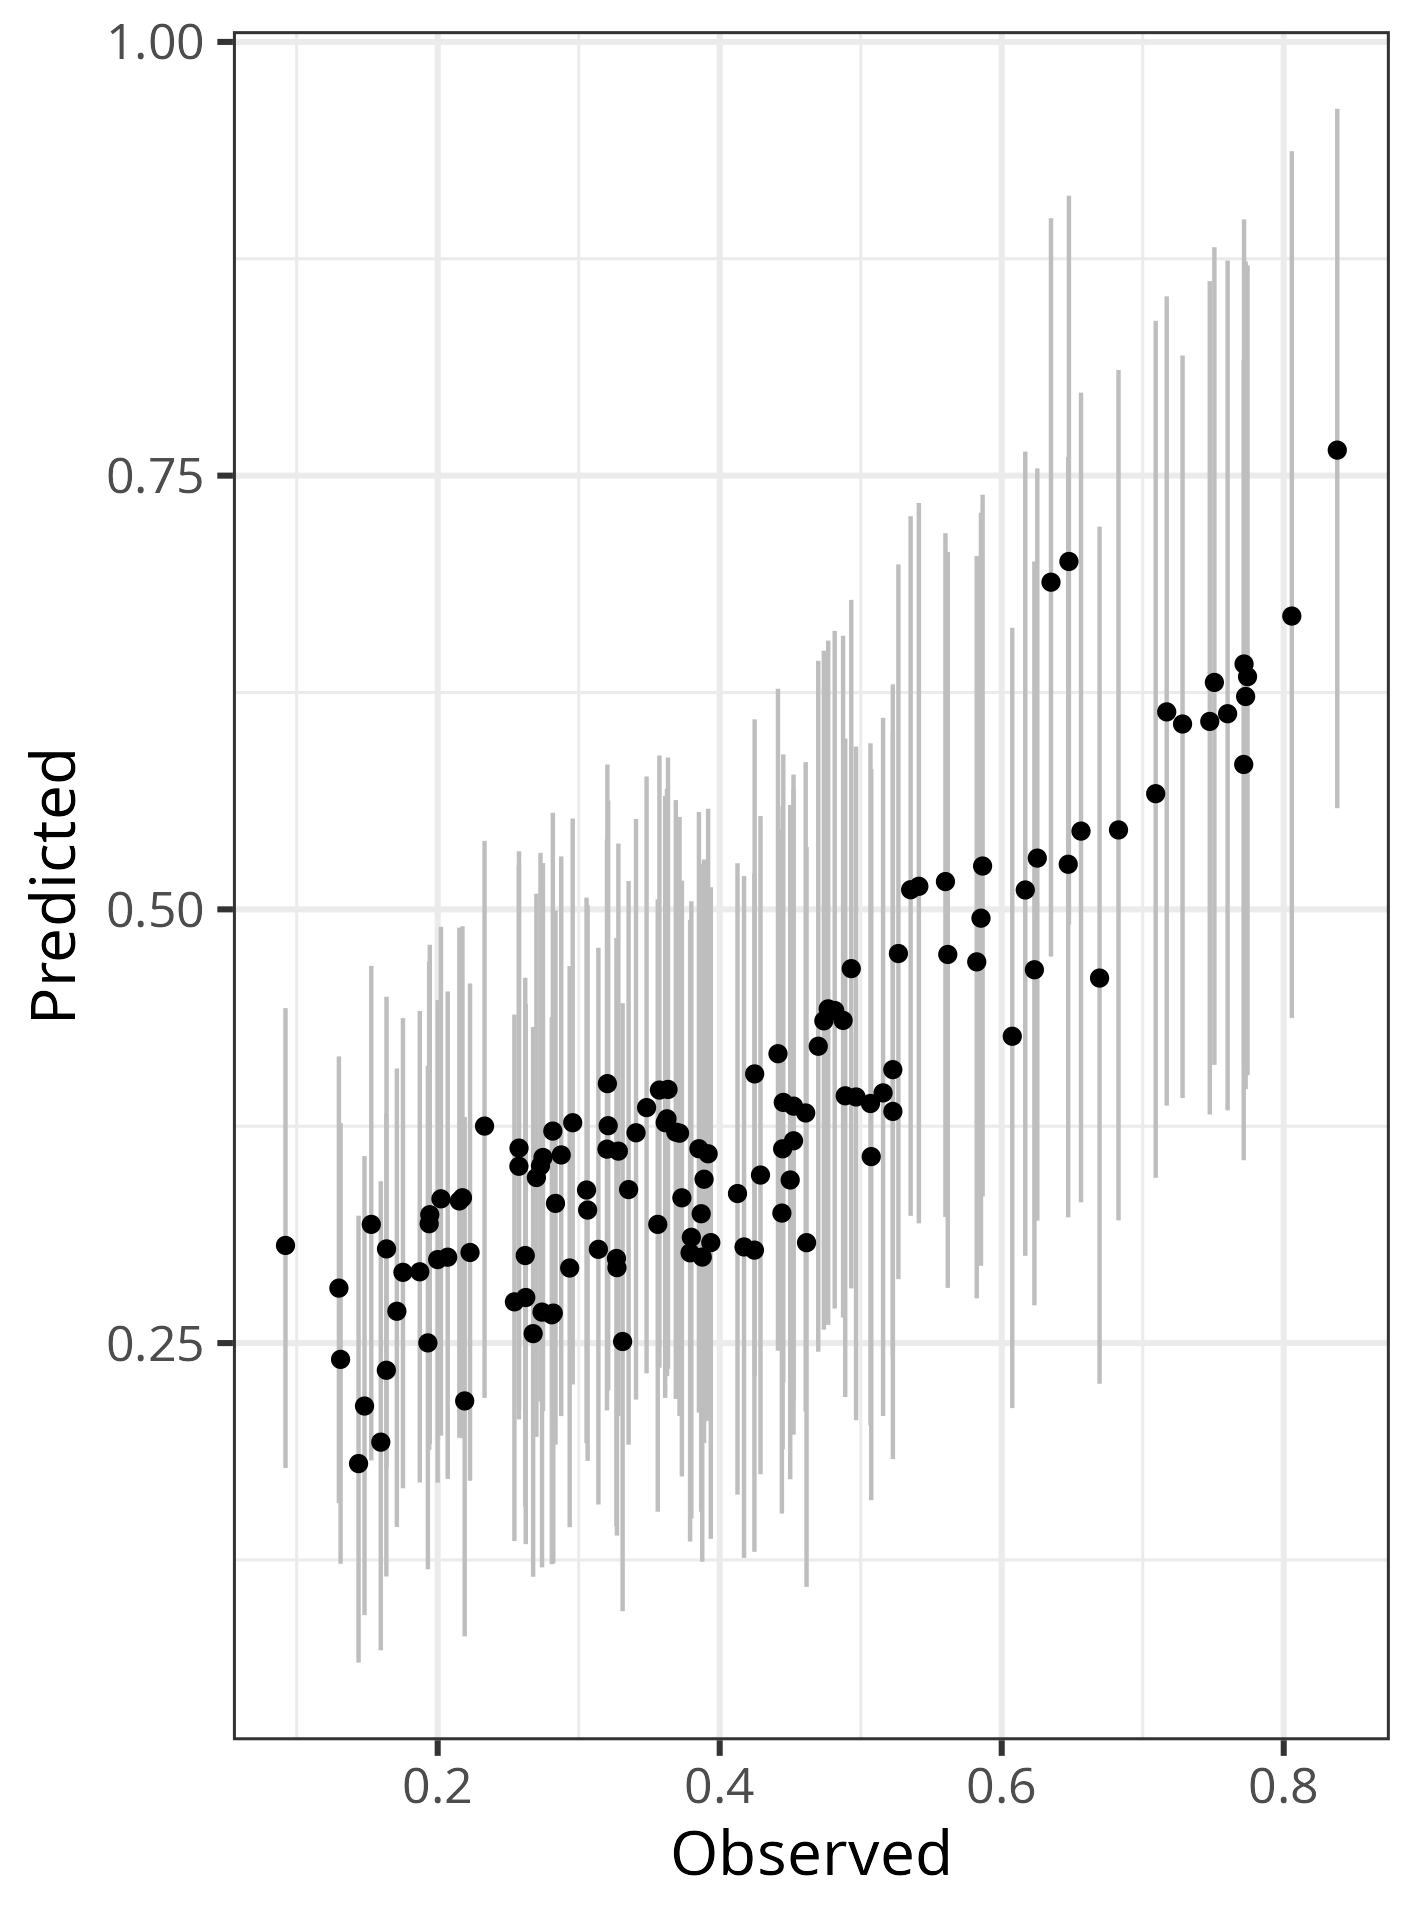
\includegraphics[width=0.5\linewidth]{README_files/figure-gfm/mobilityfitted} \caption{Fit of model to data.}\label{fig:mobilityfitted}
\end{figure}

\begin{figure}
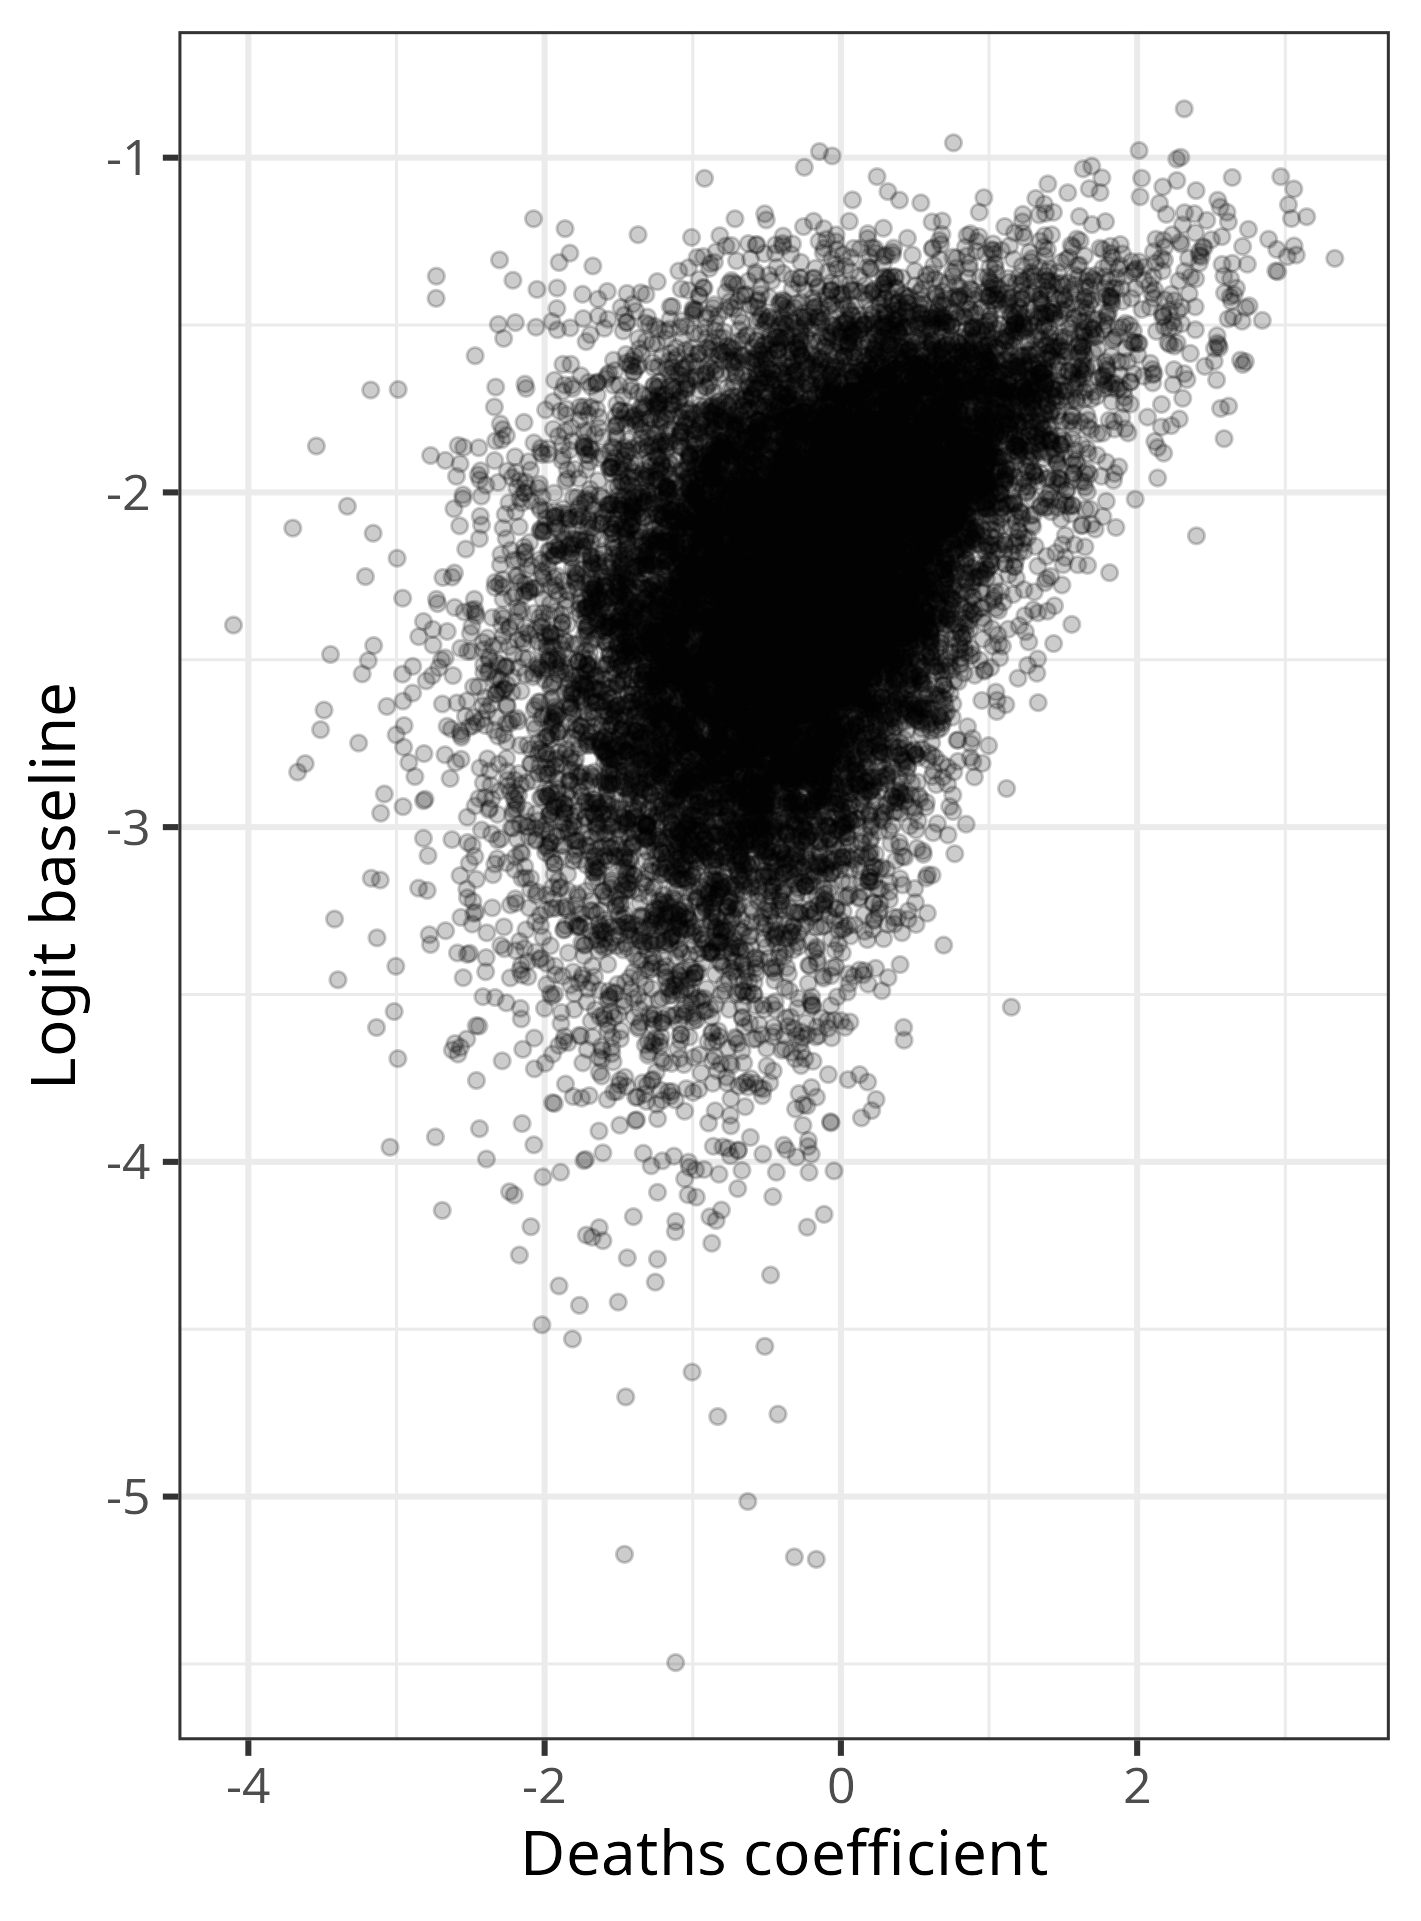
\includegraphics[width=0.5\linewidth]{README_files/figure-gfm/mobilityposterior} \caption{Posterior distribution for parameters $p^9$ and $p^8$.}\label{fig:mobilityposterior}
\end{figure}

\begin{figure}
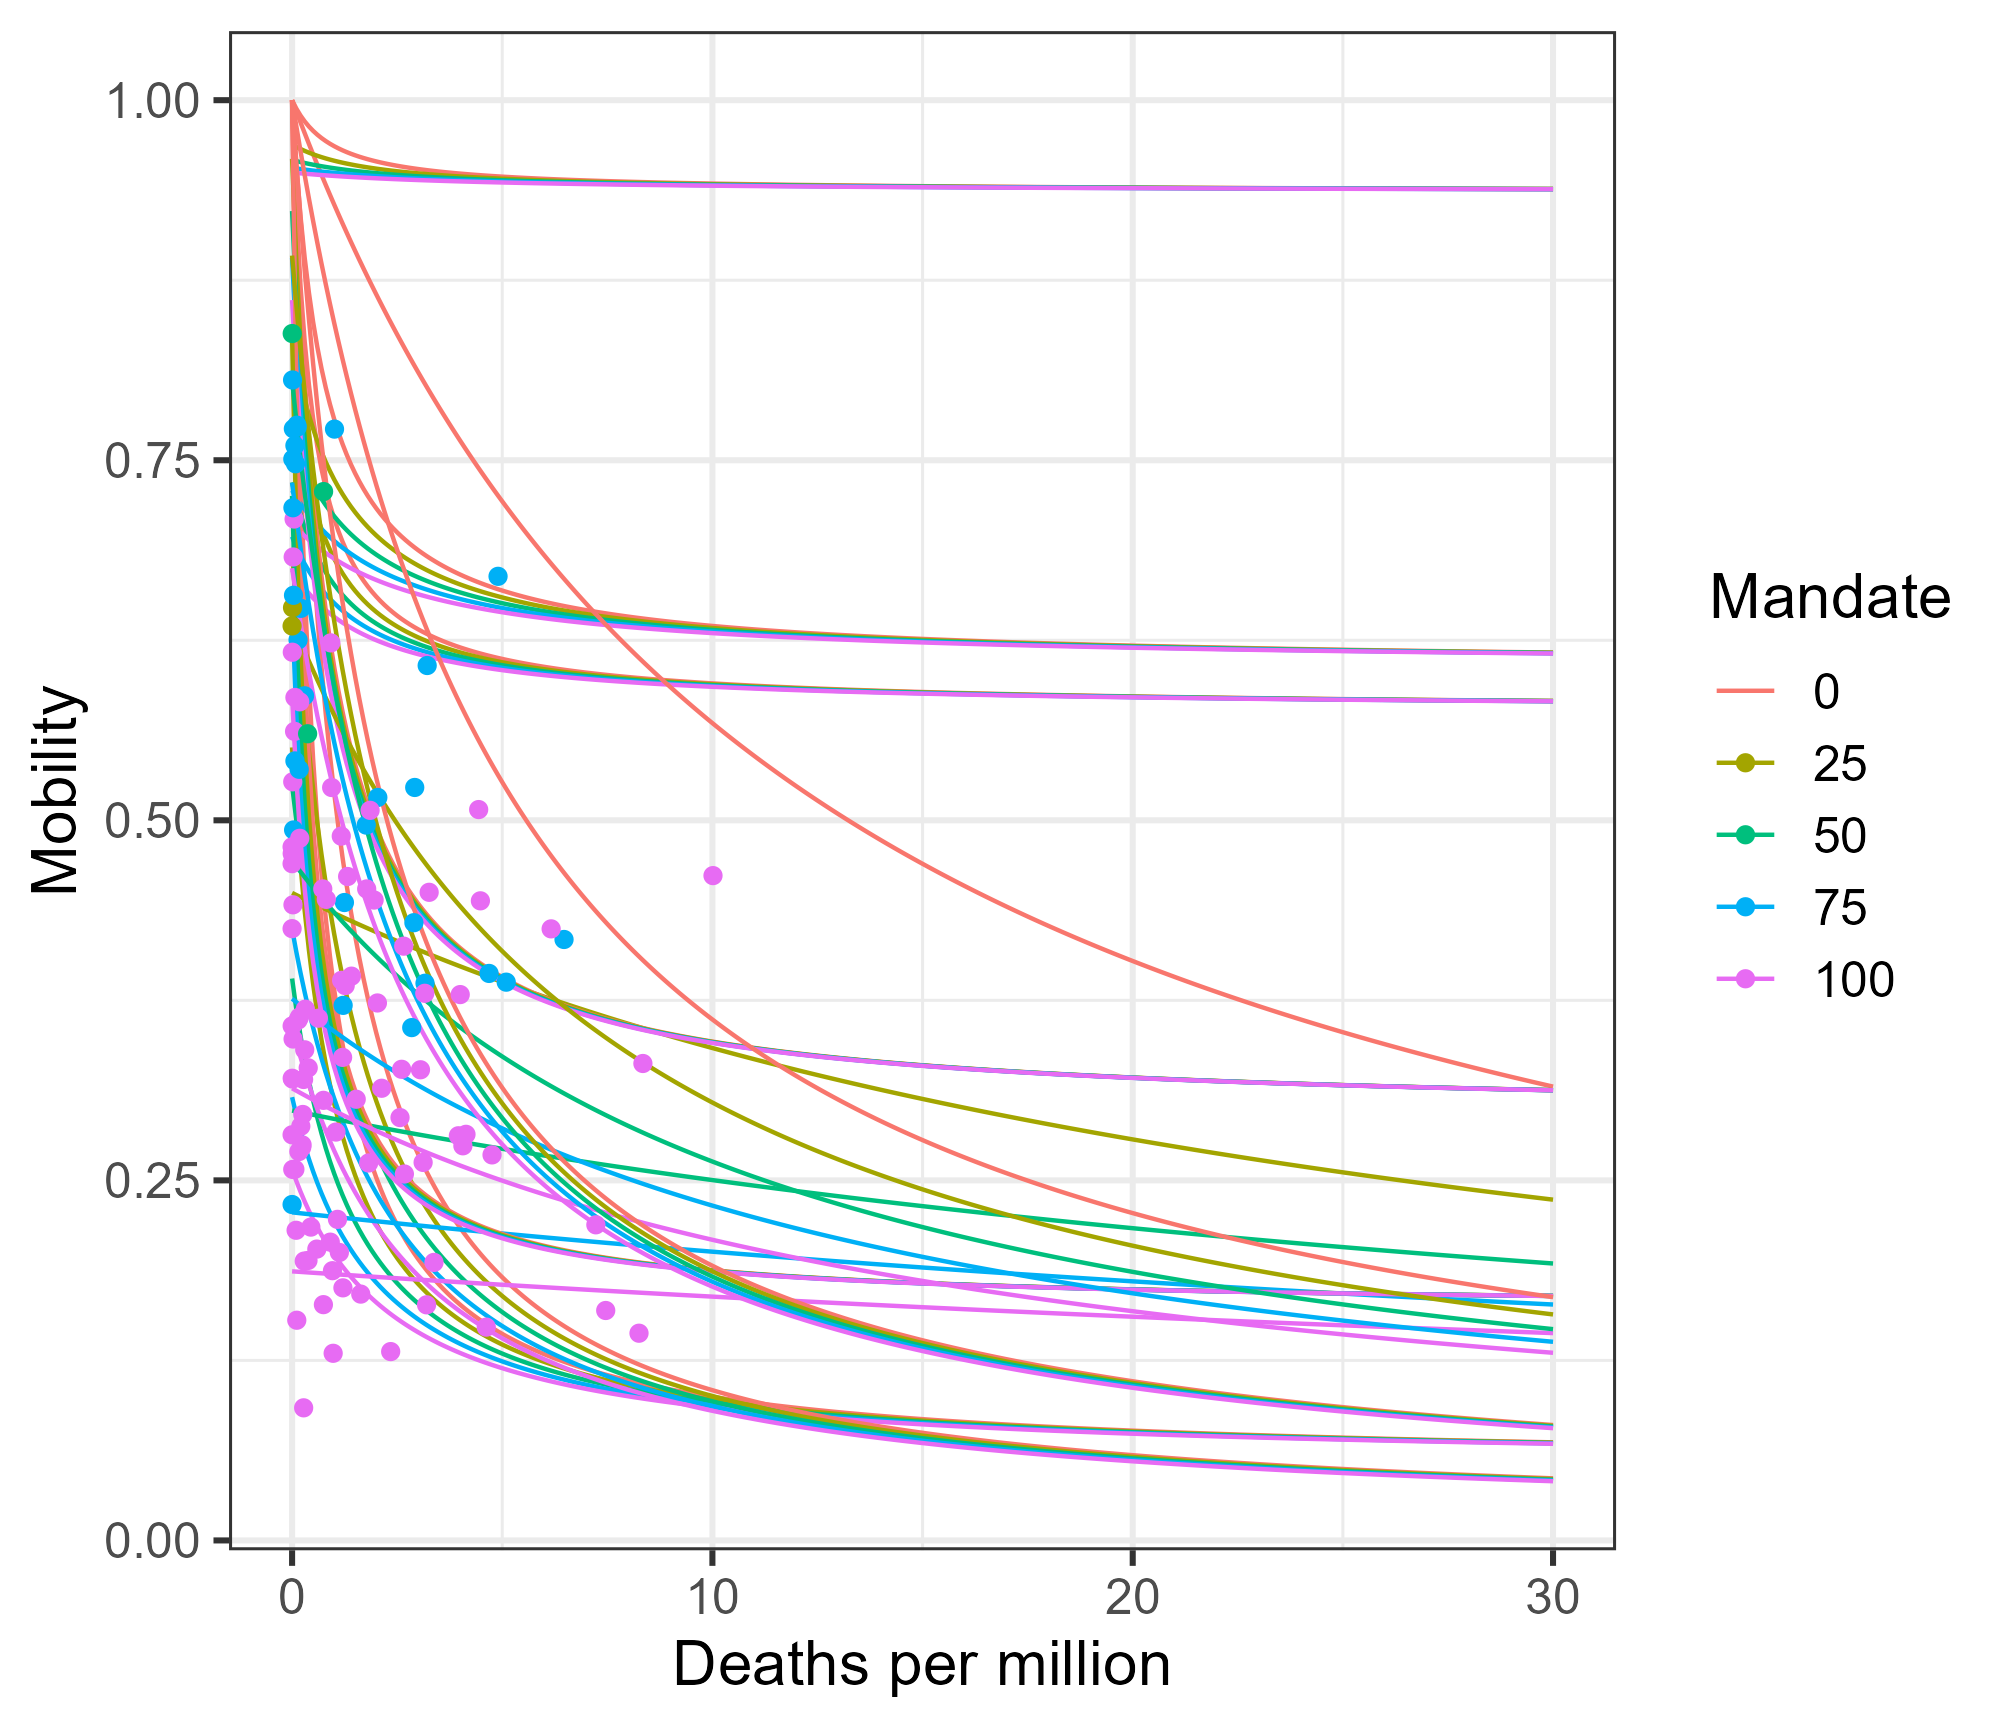
\includegraphics[width=0.5\linewidth]{README_files/figure-gfm/mobilitycurves} \caption{Sampled curves for four levels of mitigation. Data shown as points.}\label{fig:mobilitycurves}
\end{figure}

\subsection{Testing and self isolating}\label{testing-and-self-isolating}

We assume that infectious people who know their status have a compliance \(p^1\sim\text(Beta)(5,5)\) with the instruction to self isolate, starting one day into their infectious period. We assume constant infectiousness over time and that a fraction \(p^{26}\) of the symptomatic infectiousness is presymptomatic. Then the amount of infectiousness averted of symptomatic people is \(p^4=p^1(1-p^{26})\), who isolate due to the onset of symptoms. The fraction of asymptomatic cases identified by testing is \(p^2(t)\). We assume asymptomatic cases have the same probability to self isolate and that test results are returned after \(p^{17}\) days of infectiousness. Then the infectiousness that testing averts is \(p^3(t)=p^1p^2(t)\min(0,(T^{I^a:R}-p^{17})/T^{I^a:R})\).

\section{Econ model}\label{econ-model}

The economic model is measuring GDP by summing GVA over sectors and over time taking into account the extent to which sectors are open, as described in Section \ref{lost-economic-activity}.

The economy is stratified by sector following the International Standard Industrial Classification of All Economic Activities (ISIC) Rev.~4 as used by the OECD \citep{un}. Economic output is measured as the sum of gross value added (GVA) of all sectors over the epidemic period, expressed as a percentage of pre-epidemic GVA summed over the same period.

Openness comes primarily from the economic configuration which is a policy choice, mandated in response to the epidemic (see Section \ref{closure-policies}). There are potentially additional losses due to worker sickness and death (see Section \ref{lost-economic-activity}) and due to lost tourism, which is an exogenous random variable (see Section \ref{impact-of-tourism}). We do not model changes to supply or demand, reductions in consumption and labour supply due to infection avoidance of individuals, interruptions in supply chains, or changes in imports and exports.

Lost education is also quantified monetarily and constitutes an economic cost. Unlike the other losses, they are not contemporaneous with the epidemic, but losses that unfold into the future. The assumptions and equations are described in Section \ref{lost-education}.

\subsection{Impact of tourism}\label{impact-of-tourism}

\subsubsection{Food and accommodation services sector}\label{food-and-accommodation-services-sector}

As there is no ``tourism'' sector in the 45-sector classification we are using, to model the impact of changes to tourism, we identify the ``Food and accommodation services'' sector with tourism. This is imperfect. The correlation of their \% contributions to GDP is 0.64 and the order of magnitude is similar (1 to 7\% vs 2 to 10\% of GDP). The other two sectors considered (Air transport and Arts, entertainment and recreation) have little correlation with tourism in terms of \% of GDP. (See Figure \ref{fig:pairs}.)

\begin{figure}

{\centering 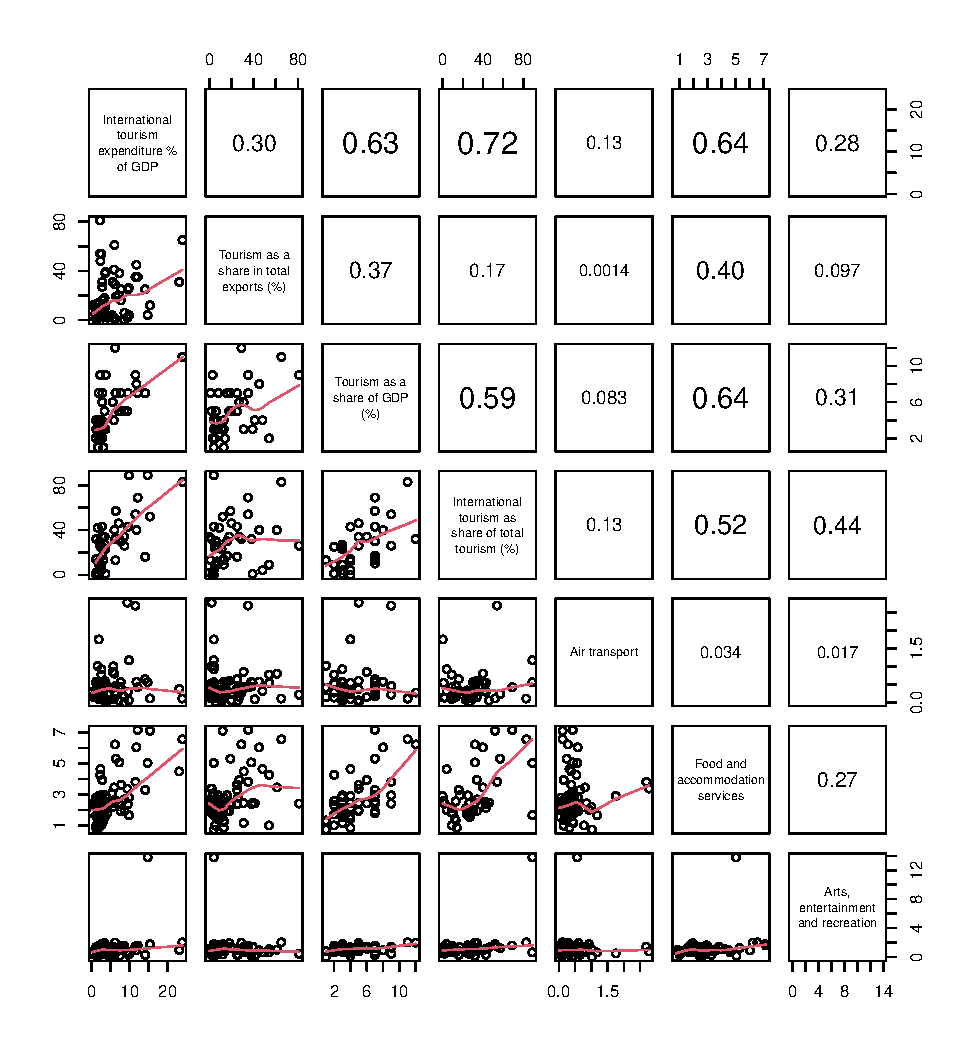
\includegraphics{README_files/figure-latex/pairs-1} 

}

\caption{Correlations between tourism-related data. First: @untourismKeyTourismStatistics2023. Second to fourth: @untourismInternationalTourismCOVID192023. Fifth to seventh: OECD.}\label{fig:pairs}
\end{figure}

\newpage

\subsubsection{Sector shrinkage as a result of the pandemic}\label{sector-shrinkage-as-a-result-of-the-pandemic}

For many countries, tourism was reduced in the COVID-19 pandemic not because of domestic mandates but because of reduced international travel. Therefore, the fraction of tourism that comes from abroad is a factor that can determine the impact of a pandemic on a country's GDP potentially independently of what happens within the country. (A useful model extension would be to include some dependence on country factors, e.g.~case numbers.)

We model mitigation via business closures, which are mandated by sector. We represent openness with values \(x\) which range from 0 to 1, 1 representing maximum openness. To capture the impact of reduced international travel, we set the maximum openness of the food and accommodation services sector to be limited by international tourism as:

\begin{Shaded}
\begin{Highlighting}[]
\NormalTok{x = \textbackslash{}min\textbackslash{}\{\textbackslash{}hat\{x\}, 1+ b(c{-}1)\textbackslash{}\}}
\end{Highlighting}
\end{Shaded}

where \(`\hat{x}`\) is the openness of the sector according to the schedule (i.e.~the sector-closure policy), \(b\) is the proportion of tourism that is international, and \(c\) is the fraction international tourism reduces to as a consequence of the pandemic. I.e. the tourism remaining is the domestic (\(1-b\)) plus that that comes in from abroad (\(bc\)).

Therefore, the contribution of the GVA of the food and accommodation services sector is limited either by the pandemic, or by the sector-closure policy - whichever is lower.

\subsubsection{Loss of international tourists}\label{loss-of-international-tourists}

We model the distribution of \(c\) using data from 2020 (Figure \ref{fig:tourismhist}, bottom-right plot). We fit to it a log-normal distribution, and find mean value -1.39 and standard deviation 0.39 (Figure \ref{fig:ytd}). We use these values as inputs for all country models.

\begin{figure}

{\centering 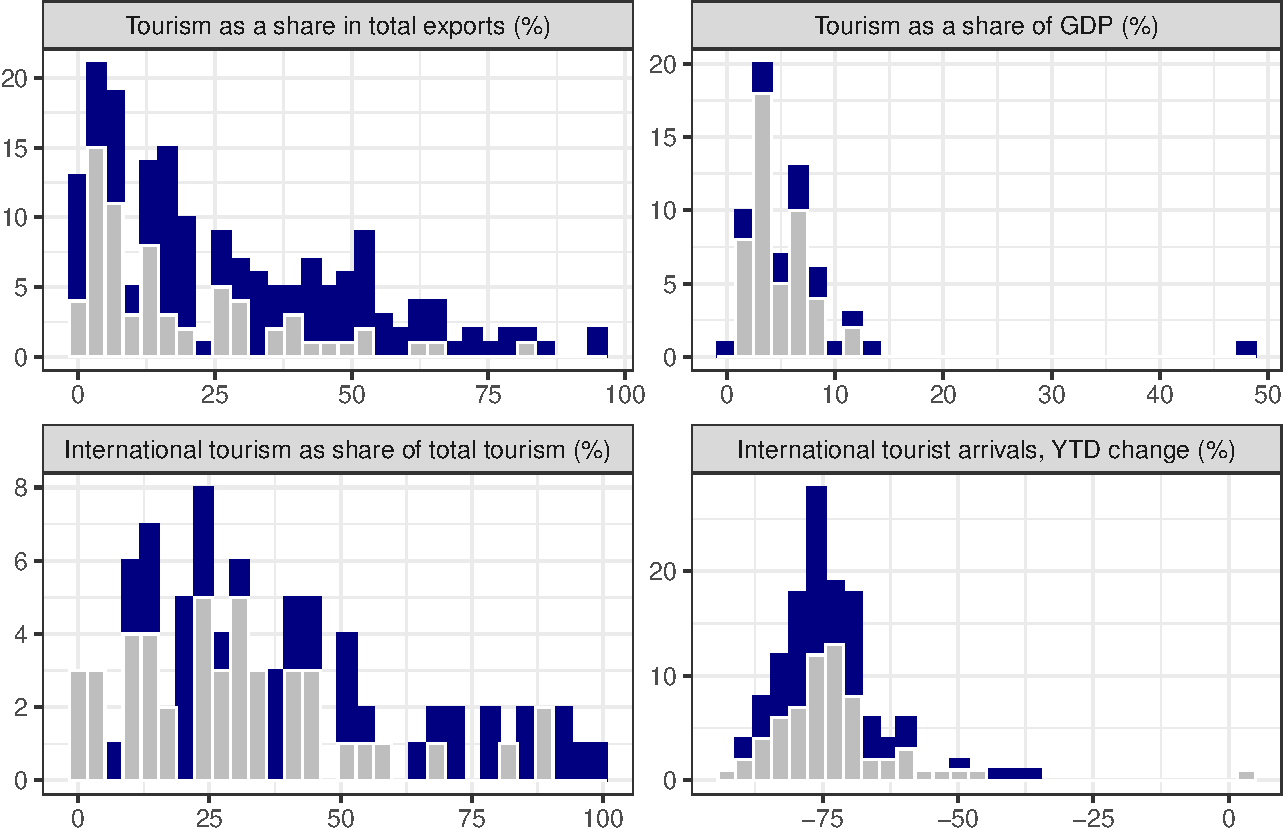
\includegraphics[width=0.5\linewidth]{README_files/figure-latex/tourismhist-1} 

}

\caption{Distributions of tourism-related data from @untourismInternationalTourismCOVID192023. In grey are the subset of countries for which we have GVA data by sector.}\label{fig:tourismhist}
\end{figure}

\begin{figure}

{\centering 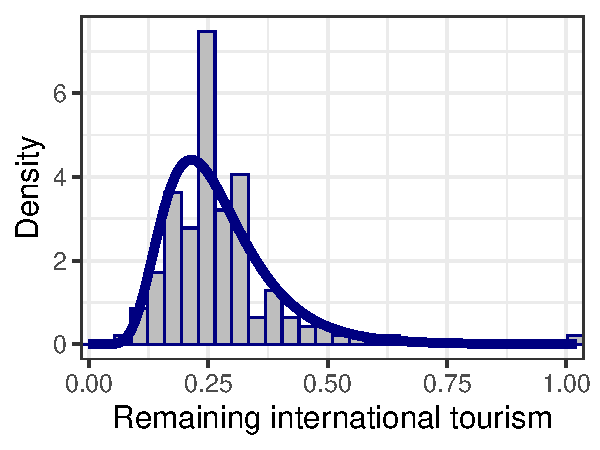
\includegraphics{README_files/figure-latex/ytd-1} 

}

\caption{Fit of log-normal distribution to loss-of-tourism data.}\label{fig:ytd}
\end{figure}

\newpage

\subsubsection{Dependence on international tourism}\label{dependence-on-international-tourism}

We model \(b\) as a function of the share of GDP that comes from the sector. Note that the data we have for this are biased towards high-income countries.

We write

\[b\sim\text{Beta}(\alpha(z),\beta(z))\]

where \(z\) is the fraction of GDP coming from the Food and accommodation sector. We learn three parameters \(p^5\), \(p^6\) and \(p^7\) to best fit the relationship between \(z\) and \(b\) in countries we have observations for:

\[p^5 = \alpha(z)+\beta(z)\]

\[p^6 z + p^7 = \frac{\alpha(z)}{\alpha(z)+\beta(z)}\]

Here, \(p^5\) controls the variance of the distribution and \(p^6\) and \(p^7\) the linear relationship between \(z\) and \(b\). Using an optimisation routine in R we find \(p^5=5.93\), \(p^6=3.66\) and \(p^7=0.099\). Results are shown in Figure \ref{fig:sectortourism}. We use these values as inputs for all country models.

\begin{figure}
\centering
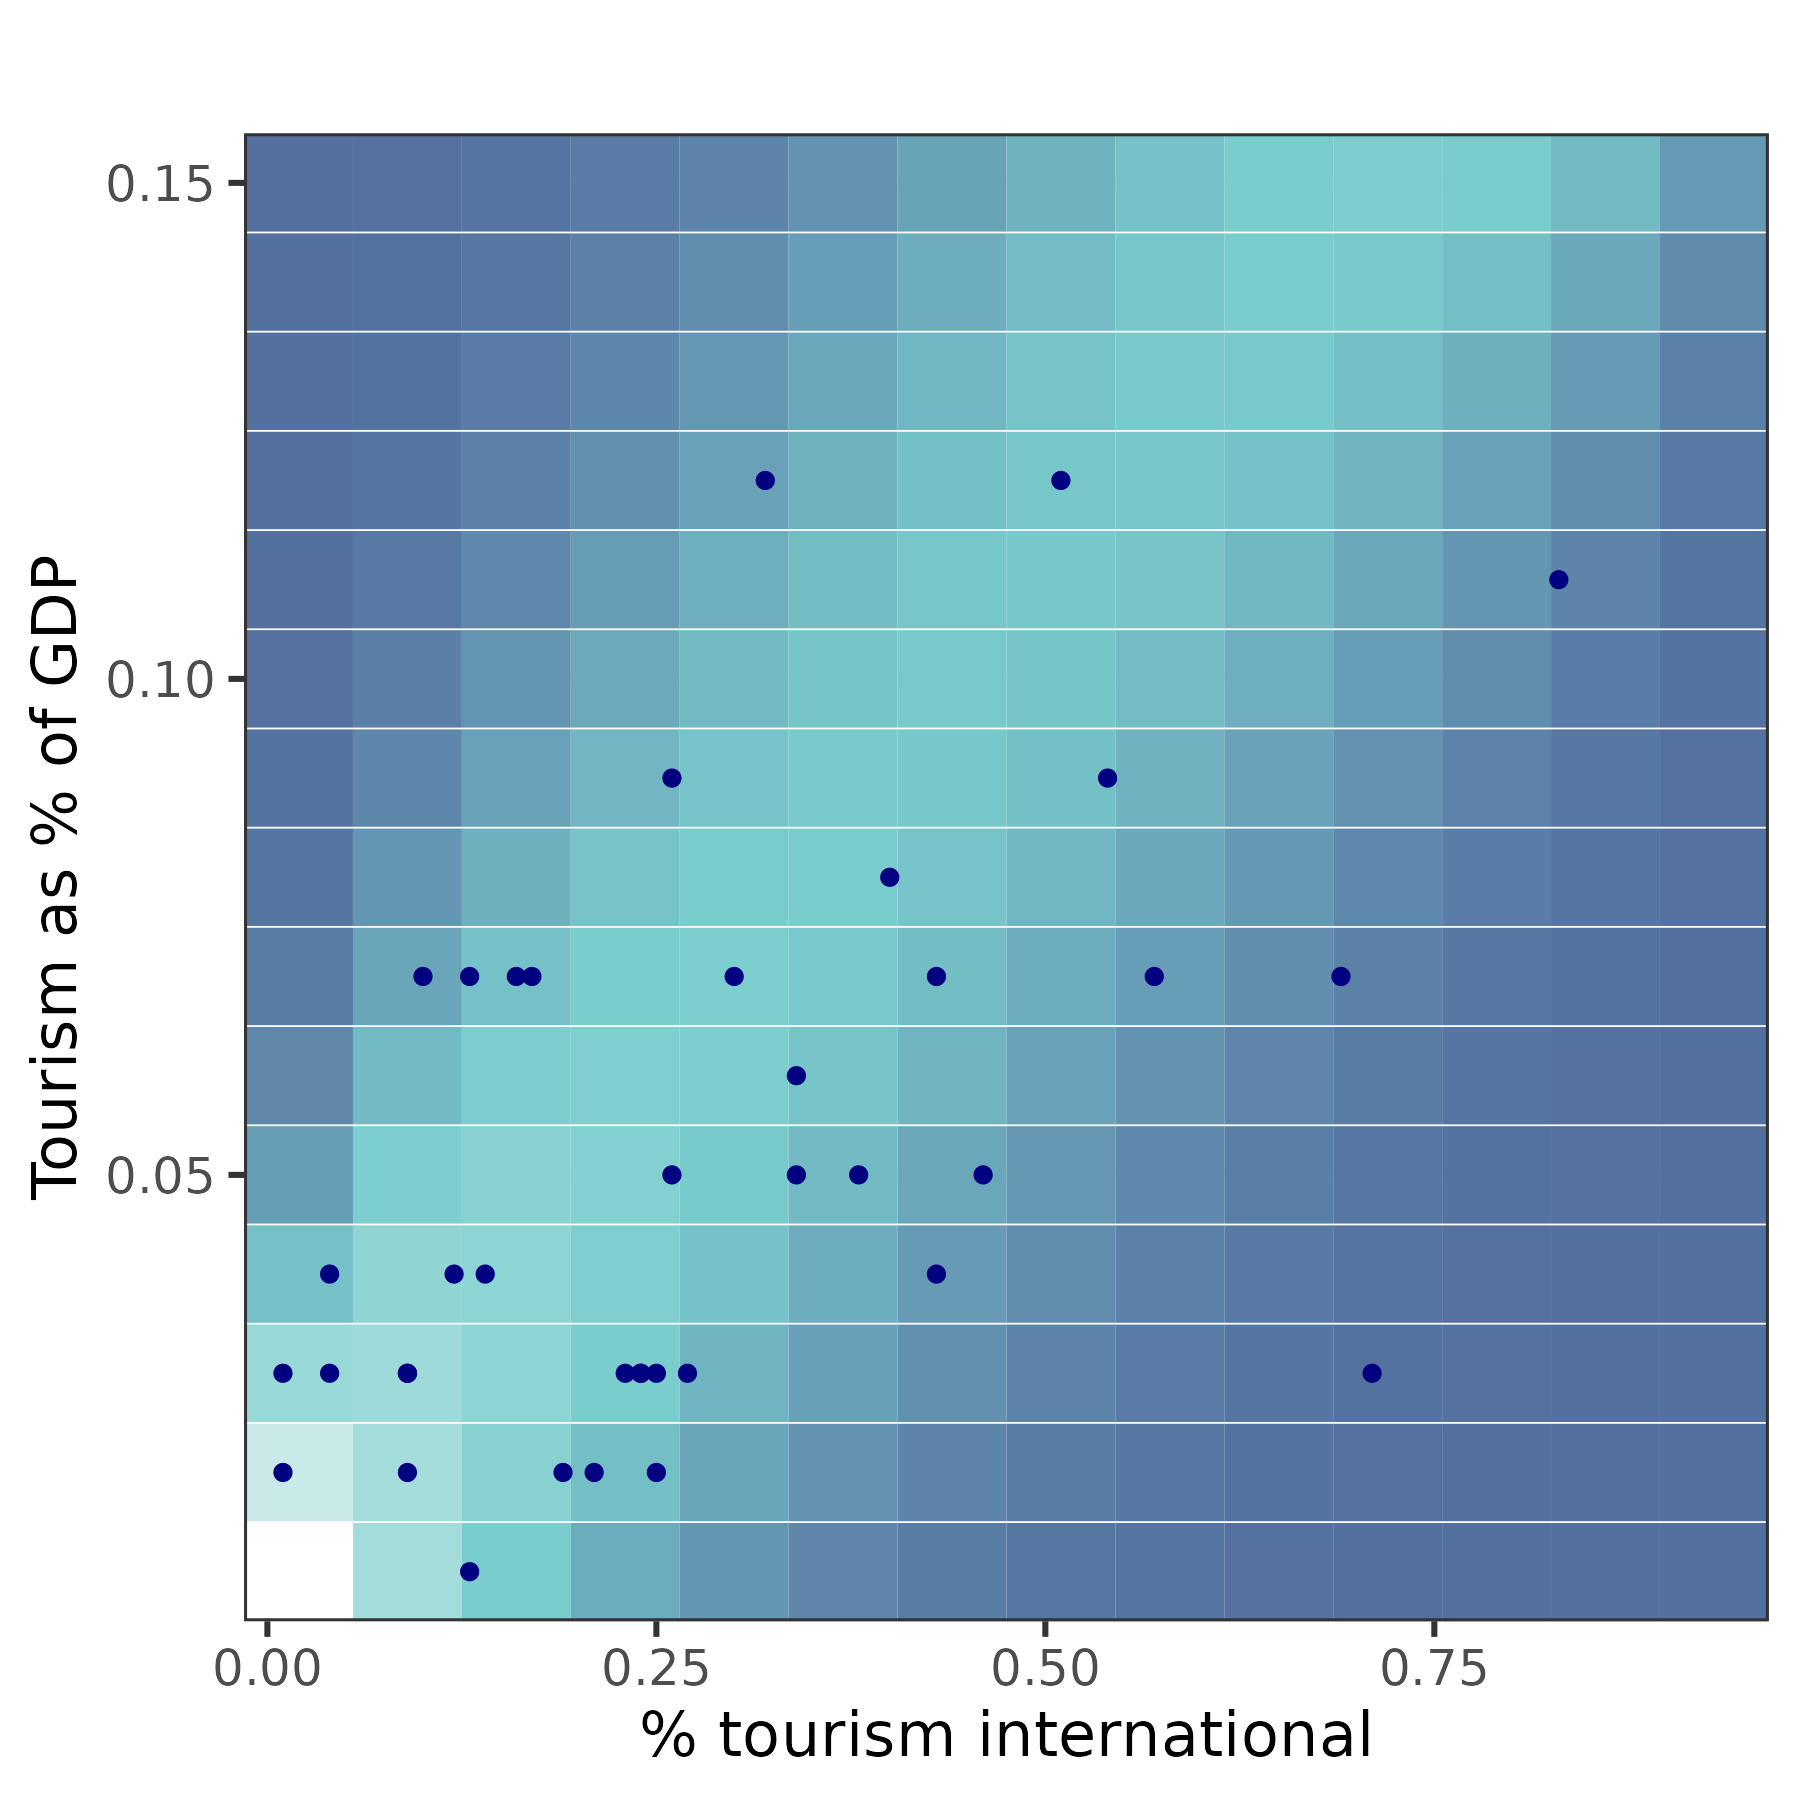
\includegraphics[width=0.4\textwidth,height=\textheight]{figures/sectortourism.png}
\caption{\label{fig:sectortourism} Predicting the percentage of tourism that comes from abroad as a function of the size of the sector. Each row represents a beta distribution whose mean is determined by the size of the sector (z). Blue points show the data we have available (grey bars in Figure \ref{fig:tourismhist}).}
\end{figure}

\newpage

\subsection{Remote working}\label{remote-working}

For each sector in each country, we have the 90\% interval for the proportion of people who can work from home from \citet{Gottlieb2021}. We assume that the value we sample within the range is related to internet infrastructure, so that a low value in one sector implies low values in all sectors. We:

\begin{itemize}
\tightlist
\item
  take the subset of countries in the income group (LLMIC / UMIC / HIC);
\item
  take the minimum of the lower bounds by sector (5\%);
\item
  take the maximum of the upper bounds by sector (95\%);
\item
  sample from a uniform distribution between these bounds, taking the same quantile for each sector.
\end{itemize}

We assume that remote working happens to its fullest extent for the whole period of mitigation for all policies.

\section{Closure policies}\label{closure-policies}

Impacts of mandated closures of businesses and schools on epidemics can be described using three factors: length, stringency, and frequency. We model mandated closures using a discrete set of predefined policies, which specify the \emph{stringency} of closures in each sector. The policies we use are the same for each country. The length and frequency of economic closures are endogenous to the model (via its epidemiology), and therefore depend on the dynamics of the epidemic that is being modelled.

We define four generic policies that might be adopted once a novel pathogen has been identified. The policies represent possible choices that range from very stringent to laissez faire, and are grounded in real-life observations. We name the policies no closures (NC) and reactive closures 1 to 3 (RC1 to RC3), and they are depicted in Figure \ref{fig:policies}, structured by the qualities that distinguish them.

The three sector-closure policies are each defined by a pair of economic configurations, and rules for moving between them. An economic configuration is a vector specifying the extent to which each sector is open, expressed as a percentage. Our economic configurations are constructed using data from three countries (Indonesia (RC1), the United Kingdom (RC2), and Australia (RC3)), via the manifest economic impacts in the wake of the COVID-19 pandemic. We take the sectoral GVA observed the COVID-19 pandemic expressed as a percentage of the values observed in the year before (OECD), i.e.~we assume that the relative GVA reflects the degree to which sectors were open.

In reality, the observed effects combined mandated closures, reductions in consumption and labour supply due to infection avoidance of individuals, interruptions in supply chains, and changes in imports and exports. However, these effects cannot be disentangled in accounts, and we do not model all of them: we use the data to represent the mandate alone. Thus we neglect two factors in our model: first, population behaviour, and second, international trade, and we ignore their impacts in the COVID-19 pandemic by subsuming all effects into the mandate. (e.g.~a pandemic that does not originate in or impact greatly China might have a much smaller economic cost).

The economic configurations define the sector closures for both the economic model and the epidemiological model. Contacts associated with sectors -- between and among workers and customers -- are scaled down with closures. GVA per sector is scaled according to economic configurations in the economic model.

For their dynamic implementation in the model, the three closure policies follow the same general pattern: they are defined by two economic configurations, which we refer to as heavy and light (where the ``heavy'' configuration has higher stringency than the ``light'' configuration; the configurations are tabulated in Table \ref{tab:eccon}). The light configuration is implemented at the response time. Thereafter, the level of closure for the three policies is mandated in response to the state of the epidemic, reverting between states as determined by the transmission dynamics. Tables \ref{tab:rulesreactive} and \ref{tab:ruleselimination} show the transitions and their conditions. RC1 and RC2 respond to hospital occupancy, allowing cases to rise and using closures to allow them to fall again. RC1 keeps school closed throughout, whereas RC2 has school open in the light configuration. RC3 aims to reduce cases and then to keep them low. All mitigation is suspended when the vaccine rollout has reached its target coverage (which is when 80\% of the eligible population have been vaccinated).

\begin{figure}
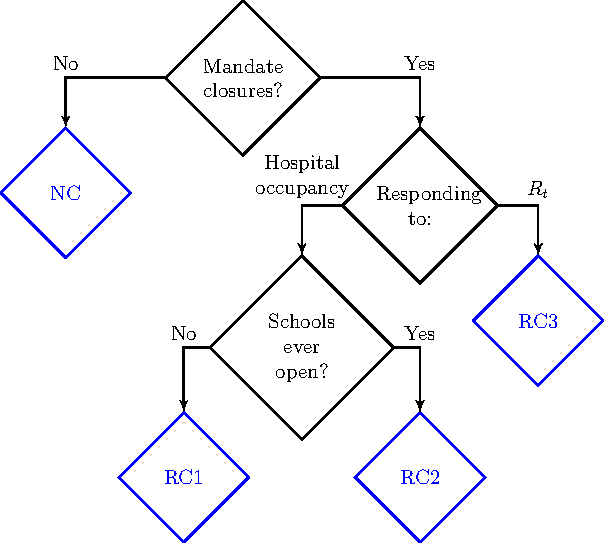
\includegraphics[width=0.5\linewidth]{README_files/figure-latex/policies-1} \caption{The four sector-closure policy options. No closures (NC) does not mandate any closures. The other three policies all implement reactive closures (RC), either in response to hospital occupancy (RC1 and RC2) or $R_t$ (RC3). The difference between RC1 and RC2 is that in RC1 schools are closed throughout, whereas in RC2 schools are fully open during the light configuration.}\label{fig:policies}
\end{figure}

The sector-closure policies are defined as follows:

\begin{itemize}
\tightlist
\item
  NC: No closures are mandated.
\item
  RC1: Schools are mandated to close to 10\% of pre-epidemic levels throughout, and other economic sectors close to the heavy-closure economic configuration when hospital occupancy reaches 95\% of its capacity, and change to the light configuration once occupancy is less than 25\% capacity.
\item
  RC2: Sectors (including the education sector) toggle between heavy and light closures reactively, as in RC1, albeit with slightly different economic configurations.
\item
  RC3: Heavy closures are chosen when \(R_t>1.2\) and light closures when \(R_t<0.95\). Closures are maintained until \(R_t<1\) without closures, or vaccination targets are reached.
\end{itemize}

All policies assume there is testing (Section \ref{testing-and-self-isolating}), working from home (Section \ref{remote-working}), and uncosted transmission reductions from behavioural changes (Section \ref{uncosted-transmission-reductions}), which impact epidemiological outcomes. They do not directly impact economic outcomes, but indirectly may reduce the need for closures because of reduced incidence.

\begin{longtable}[]{@{}
  >{\raggedright\arraybackslash}p{(\columnwidth - 6\tabcolsep) * \real{0.2500}}
  >{\raggedright\arraybackslash}p{(\columnwidth - 6\tabcolsep) * \real{0.2500}}
  >{\raggedright\arraybackslash}p{(\columnwidth - 6\tabcolsep) * \real{0.2500}}
  >{\raggedright\arraybackslash}p{(\columnwidth - 6\tabcolsep) * \real{0.2500}}@{}}
\caption{\label{tab:rulesreactive} State transition rules for policies RC1 and RC2. See Table \ref{tab:eccon} for details of closures.}\tabularnewline
\toprule\noalign{}
\begin{minipage}[b]{\linewidth}\raggedright
From/to
\end{minipage} & \begin{minipage}[b]{\linewidth}\raggedright
No closures
\end{minipage} & \begin{minipage}[b]{\linewidth}\raggedright
Light closures
\end{minipage} & \begin{minipage}[b]{\linewidth}\raggedright
Heavy closures
\end{minipage} \\
\midrule\noalign{}
\endfirsthead
\toprule\noalign{}
\begin{minipage}[b]{\linewidth}\raggedright
From/to
\end{minipage} & \begin{minipage}[b]{\linewidth}\raggedright
No closures
\end{minipage} & \begin{minipage}[b]{\linewidth}\raggedright
Light closures
\end{minipage} & \begin{minipage}[b]{\linewidth}\raggedright
Heavy closures
\end{minipage} \\
\midrule\noalign{}
\endhead
\bottomrule\noalign{}
\endlastfoot
\textbf{No closures} & & t \(\geq\) response time AND Hospital occupancy \textgreater{} 95\% capacity & \\
\textbf{Light closures} & (Growth rate \textless{} 0.025 OR Hospital occupancy \textless{} 25\% capacity) AND vaccine rollout complete OR \(R_t(M(\textbf{1})) < 1\) & & Hospital occupancy \textgreater{} 95\% capacity \\
\textbf{Heavy closures} & & Hospital occupancy \textless{} 25\% capacity AND t \textgreater{} 7 + last change time & \\
\end{longtable}

\begin{longtable}[]{@{}
  >{\raggedright\arraybackslash}p{(\columnwidth - 6\tabcolsep) * \real{0.2500}}
  >{\raggedright\arraybackslash}p{(\columnwidth - 6\tabcolsep) * \real{0.2500}}
  >{\raggedright\arraybackslash}p{(\columnwidth - 6\tabcolsep) * \real{0.2500}}
  >{\raggedright\arraybackslash}p{(\columnwidth - 6\tabcolsep) * \real{0.2500}}@{}}
\caption{\label{tab:ruleselimination} State transition rules for policy RC3. See Table \ref{tab:eccon} for details of closures.}\tabularnewline
\toprule\noalign{}
\begin{minipage}[b]{\linewidth}\raggedright
From/to
\end{minipage} & \begin{minipage}[b]{\linewidth}\raggedright
No closures
\end{minipage} & \begin{minipage}[b]{\linewidth}\raggedright
Light closures
\end{minipage} & \begin{minipage}[b]{\linewidth}\raggedright
Heavy closures
\end{minipage} \\
\midrule\noalign{}
\endfirsthead
\toprule\noalign{}
\begin{minipage}[b]{\linewidth}\raggedright
From/to
\end{minipage} & \begin{minipage}[b]{\linewidth}\raggedright
No closures
\end{minipage} & \begin{minipage}[b]{\linewidth}\raggedright
Light closures
\end{minipage} & \begin{minipage}[b]{\linewidth}\raggedright
Heavy closures
\end{minipage} \\
\midrule\noalign{}
\endhead
\bottomrule\noalign{}
\endlastfoot
\textbf{No closures} & & t \(\geq\) response time OR Hospital occupancy \textgreater{} 95\% capacity & \\
\textbf{Light closures} & Vaccine rollout complete OR \(R_t(M(\textbf{1})) < 1\) & & \(R_t > 1.2\) \\
\textbf{Heavy closures} & Vaccine rollout complete OR \(R_t(M(\textbf{1})) < 1\) & \(R_t(M(x_{\text{light closure}})) < 0.95\) AND t \textgreater{} 7 + last change time & \\
\end{longtable}

\begin{longtable}[]{@{}
  >{\centering\arraybackslash}p{(\columnwidth - 12\tabcolsep) * \real{0.2444}}
  >{\centering\arraybackslash}p{(\columnwidth - 12\tabcolsep) * \real{0.1259}}
  >{\centering\arraybackslash}p{(\columnwidth - 12\tabcolsep) * \real{0.1259}}
  >{\centering\arraybackslash}p{(\columnwidth - 12\tabcolsep) * \real{0.1259}}
  >{\centering\arraybackslash}p{(\columnwidth - 12\tabcolsep) * \real{0.1259}}
  >{\centering\arraybackslash}p{(\columnwidth - 12\tabcolsep) * \real{0.1259}}
  >{\centering\arraybackslash}p{(\columnwidth - 12\tabcolsep) * \real{0.1259}}@{}}
\caption{Economic configurations used to implement strategies. Values are the openness of the sector expressed as a percentage. RC3 values are taken from Australia. Lockdown and RC2 values are taken from the UK. RC1 values are taken from Indonesia. \label{tab:eccon}}\tabularnewline
\toprule\noalign{}
\begin{minipage}[b]{\linewidth}\centering
Sector
\end{minipage} & \begin{minipage}[b]{\linewidth}\centering
Heavy closures
\end{minipage} & \begin{minipage}[b]{\linewidth}\centering
Light closures
\end{minipage} & \begin{minipage}[b]{\linewidth}\centering
Heavy closures
\end{minipage} & \begin{minipage}[b]{\linewidth}\centering
Light closures
\end{minipage} & \begin{minipage}[b]{\linewidth}\centering
Heavy closures
\end{minipage} & \begin{minipage}[b]{\linewidth}\centering
Light closures
\end{minipage} \\
\midrule\noalign{}
\endfirsthead
\toprule\noalign{}
\begin{minipage}[b]{\linewidth}\centering
Sector
\end{minipage} & \begin{minipage}[b]{\linewidth}\centering
Heavy closures
\end{minipage} & \begin{minipage}[b]{\linewidth}\centering
Light closures
\end{minipage} & \begin{minipage}[b]{\linewidth}\centering
Heavy closures
\end{minipage} & \begin{minipage}[b]{\linewidth}\centering
Light closures
\end{minipage} & \begin{minipage}[b]{\linewidth}\centering
Heavy closures
\end{minipage} & \begin{minipage}[b]{\linewidth}\centering
Light closures
\end{minipage} \\
\midrule\noalign{}
\endhead
\bottomrule\noalign{}
\endlastfoot
Agriculture, hunting, forestry & 86 & 100 & 86 & 88 & 100 & 100 \\
Fishing and aquaculture & 86 & 100 & 86 & 88 & 100 & 100 \\
Mining and quarrying, energy
producing products & 90 & 100 & 90 & 91 & 67 & 79 \\
Mining and quarrying,
non-energy producing products & 90 & 100 & 90 & 91 & 100 & 100 \\
Mining support service
activities & 90 & 100 & 90 & 91 & 100 & 100 \\
Food products, beverages and
tobacco & 70 & 100 & 70 & 94 & 100 & 100 \\
Textiles, textile products,
leather and footwear & 70 & 98 & 70 & 94 & 89 & 92 \\
Wood and products of wood and
cork & 70 & 98 & 70 & 94 & 100 & 95 \\
Paper products and printing & 70 & 98 & 70 & 94 & 100 & 98 \\
Coke and refined petroleum
products & 70 & 88 & 70 & 94 & 87 & 88 \\
Chemical and chemical products & 70 & 88 & 70 & 94 & 100 & 100 \\
Pharmaceuticals, medicinal
chemical and botanical
products & 70 & 88 & 70 & 94 & 100 & 100 \\
Rubber and plastics products & 70 & 88 & 70 & 94 & 87 & 100 \\
Other non-metallic mineral
products & 70 & 88 & 70 & 94 & 92 & 89 \\
Basic metals & 70 & 100 & 70 & 94 & 100 & 100 \\
Fabricated metal products & 70 & 100 & 70 & 94 & 90 & 100 \\
Computer, electronic and
optical equipment & 70 & 100 & 70 & 94 & 90 & 100 \\
Electrical equipment & 70 & 100 & 70 & 94 & 90 & 100 \\
Machinery and equipment, nec & 70 & 100 & 70 & 94 & 89 & 95 \\
Motor vehicles, trailers and
semi-trailers & 70 & 100 & 70 & 94 & 66 & 82 \\
Other transport equipment & 70 & 100 & 70 & 94 & 66 & 82 \\
Manufacturing nec; repair and
installation of machinery and
equipment & 70 & 98 & 70 & 94 & 98 & 100 \\
Electricity, gas, steam and
air conditioning supply & 89 & 97 & 89 & 100 & 94 & 94 \\
Water supply; sewerage, waste
management and remediation
activities & 92 & 97 & 92 & 98 & 100 & 100 \\
Construction & 56 & 94 & 56 & 92 & 95 & 95 \\
Wholesale and retail trade;
repair of motor vehicles & 64 & 100 & 64 & 100 & 92 & 97 \\
Land transport and transport
via pipelines & 63 & 100 & 63 & 82 & 83 & 100 \\
Water transport & 63 & 100 & 63 & 82 & 81 & 98 \\
Air transport & 63 & 18 & 63 & 82 & 16 & 42 \\
Warehousing and support
activities for transportation & 63 & 91 & 63 & 82 & 64 & 91 \\
Postal and courier activities & 63 & 91 & 63 & 82 & 64 & 91 \\
Accommodation and food service
activities & 10 & 92 & 10 & 85 & 77 & 91 \\
Publishing, audiovisual and
broadcasting activities & 88 & 100 & 88 & 91 & 100 & 100 \\
Telecommunications & 88 & 100 & 88 & 91 & 100 & 100 \\
IT and other information
services & 88 & 100 & 88 & 91 & 100 & 100 \\
Financial and insurance
activities & 94 & 100 & 94 & 96 & 100 & 100 \\
Real estate activities & 98 & 100 & 98 & 98 & 100 & 100 \\
Professional, scientific and
technical activities & 85 & 100 & 85 & 92 & 90 & 95 \\
Administrative and support
services & 66 & 90 & 66 & 80 & 90 & 95 \\
Public administration and
defence; compulsory social
security & 100 & 100 & 100 & 100 & 96 & 100 \\
Education & 10 & 100 & 10 & 100 & 10 & 10 \\
Human health and social work
activities & 75 & 100 & 75 & 92 & 100 & 100 \\
Arts, entertainment and
recreation & 55 & 94 & 55 & 71 & 90 & 96 \\
Other service activities & 54 & 94 & 54 & 83 & 90 & 96 \\
Activities of households as
employers; undifferentiated
goods- and services-producing
activities of households for
own use & 49 & 94 & 49 & 53 & 90 & 96 \\
\end{longtable}

\section{Pathogen profiles}\label{pathogen-profiles}

We sample pathogen profiles by defining distributions over the pathogen parameters. The distributions are made using sourced data (Table \ref{tab:pathogenprofile}), and are described in Table \ref{tab:pathogenparameters}. Age profiles for severity rates are shown in Figure \ref{fig:ratesbyage}. We sample parameter values from distributions informed by the seven pathogen profiles. R\(_0\) is truncated at 1.5 and 4 following \citet{whittakerQuantifyingImpactBroadly2024}.

\begin{longtable}[]{@{}
  >{\centering\arraybackslash}p{(\columnwidth - 14\tabcolsep) * \real{0.1988}}
  >{\centering\arraybackslash}p{(\columnwidth - 14\tabcolsep) * \real{0.0807}}
  >{\centering\arraybackslash}p{(\columnwidth - 14\tabcolsep) * \real{0.1056}}
  >{\centering\arraybackslash}p{(\columnwidth - 14\tabcolsep) * \real{0.1056}}
  >{\centering\arraybackslash}p{(\columnwidth - 14\tabcolsep) * \real{0.1056}}
  >{\centering\arraybackslash}p{(\columnwidth - 14\tabcolsep) * \real{0.1429}}
  >{\centering\arraybackslash}p{(\columnwidth - 14\tabcolsep) * \real{0.1304}}
  >{\centering\arraybackslash}p{(\columnwidth - 14\tabcolsep) * \real{0.1304}}@{}}
\caption{Pathogen profiles. IHR: infection hospitalisation rate. IFR: infection fatality rate. \label{tab:pathogenprofile}}\tabularnewline
\toprule\noalign{}
\begin{minipage}[b]{\linewidth}\centering
~
\end{minipage} & \begin{minipage}[b]{\linewidth}\centering
SARS-CoV-1
\end{minipage} & \begin{minipage}[b]{\linewidth}\centering
Influenza 2009
\end{minipage} & \begin{minipage}[b]{\linewidth}\centering
Influenza 1957
\end{minipage} & \begin{minipage}[b]{\linewidth}\centering
Influenza 1918
\end{minipage} & \begin{minipage}[b]{\linewidth}\centering
SARS-CoV-2 pre-alpha
\end{minipage} & \begin{minipage}[b]{\linewidth}\centering
SARS-CoV-2 omicron
\end{minipage} & \begin{minipage}[b]{\linewidth}\centering
SARS-CoV-2 delta
\end{minipage} \\
\midrule\noalign{}
\endfirsthead
\toprule\noalign{}
\begin{minipage}[b]{\linewidth}\centering
~
\end{minipage} & \begin{minipage}[b]{\linewidth}\centering
SARS-CoV-1
\end{minipage} & \begin{minipage}[b]{\linewidth}\centering
Influenza 2009
\end{minipage} & \begin{minipage}[b]{\linewidth}\centering
Influenza 1957
\end{minipage} & \begin{minipage}[b]{\linewidth}\centering
Influenza 1918
\end{minipage} & \begin{minipage}[b]{\linewidth}\centering
SARS-CoV-2 pre-alpha
\end{minipage} & \begin{minipage}[b]{\linewidth}\centering
SARS-CoV-2 omicron
\end{minipage} & \begin{minipage}[b]{\linewidth}\centering
SARS-CoV-2 delta
\end{minipage} \\
\midrule\noalign{}
\endhead
\bottomrule\noalign{}
\endlastfoot
\textbf{IHR in 0-4 age group} & 0.058 & 0.0047 & 0.0009 & 0.12 & 0.000016 & 0.000033 & 0.00003 \\
\textbf{IHR in 5-9 age group} & 0.058 & 0.0018 & 0.0009 & 0.021 & 0.000016 & 0.000033 & 0.00003 \\
\textbf{IHR in 10-14 age group} & 0.058 & 0.0018 & 0.0009 & 0.026 & 0.00041 & 0.00059 & 0.00075 \\
\textbf{IHR in 15-19 age group} & 0.058 & 0.0018 & 0.0009 & 0.053 & 0.00041 & 0.00059 & 0.00075 \\
\textbf{IHR in 20-24 age group} & 0.082 & 0.0018 & 0.0009 & 0.091 & 0.01 & 0.0083 & 0.019 \\
\textbf{IHR in 25-29 age group} & 0.082 & 0.0038 & 0.0009 & 0.16 & 0.01 & 0.0083 & 0.019 \\
\textbf{IHR in 30-34 age group} & 0.082 & 0.0038 & 0.0009 & 0.13 & 0.034 & 0.02 & 0.063 \\
\textbf{IHR in 35-39 age group} & 0.082 & 0.0038 & 0.0009 & 0.12 & 0.034 & 0.02 & 0.063 \\
\textbf{IHR in 40-44 age group} & 0.3 & 0.0038 & 0.0009 & 0.088 & 0.042 & 0.016 & 0.079 \\
\textbf{IHR in 45-49 age group} & 0.3 & 0.0038 & 0.023 & 0.064 & 0.042 & 0.016 & 0.079 \\
\textbf{IHR in 50-54 age group} & 0.3 & 0.0071 & 0.023 & 0.088 & 0.082 & 0.021 & 0.15 \\
\textbf{IHR in 55-59 age group} & 0.3 & 0.0071 & 0.023 & 0.063 & 0.082 & 0.021 & 0.15 \\
\textbf{IHR in 60-64 age group} & 0.87 & 0.0071 & 0.023 & 0.16 & 0.12 & 0.031 & 0.22 \\
\textbf{IHR in 65-69 age group} & 0.87 & 0.01 & 0.18 & 0.22 & 0.12 & 0.031 & 0.22 \\
\textbf{IHR in 70-74 age group} & 0.87 & 0.01 & 0.18 & 0.26 & 0.17 & 0.061 & 0.31 \\
\textbf{IHR in 75-79 age group} & 0.87 & 0.01 & 0.18 & 0.26 & 0.17 & 0.061 & 0.31 \\
\textbf{IHR in 80+ age group} & 0.6 & 0.01 & 0.18 & 0.26 & 0.18 & 0.11 & 0.34 \\
\textbf{IFR in 0-4 age group} & 0.015 & 0.00018 & 0.000067 & 0.015 & 0.000016 & 0.000033 & 0.00003 \\
\textbf{IFR in 5-9 age group} & 0.015 & 0.000074 & 0.000067 & 0.0027 & 0.000016 & 0.000033 & 0.00003 \\
\textbf{IFR in 10-14 age group} & 0.015 & 0.000074 & 0.000067 & 0.0032 & 0.00007 & 0.0001 & 0.00013 \\
\textbf{IFR in 15-19 age group} & 0.015 & 0.00008 & 0.000067 & 0.0066 & 0.00007 & 0.0001 & 0.00013 \\
\textbf{IFR in 20-24 age group} & 0.021 & 0.00008 & 0.000067 & 0.011 & 0.00031 & 0.00025 & 0.00057 \\
\textbf{IFR in 25-29 age group} & 0.021 & 0.0002 & 0.000067 & 0.02 & 0.00031 & 0.00025 & 0.00057 \\
\textbf{IFR in 30-34 age group} & 0.021 & 0.0002 & 0.000067 & 0.017 & 0.00084 & 0.00048 & 0.0016 \\
\textbf{IFR in 35-39 age group} & 0.021 & 0.0002 & 0.000067 & 0.015 & 0.00084 & 0.00048 & 0.0016 \\
\textbf{IFR in 40-44 age group} & 0.077 & 0.0002 & 0.000067 & 0.011 & 0.0016 & 0.0006 & 0.003 \\
\textbf{IFR in 45-49 age group} & 0.077 & 0.00043 & 0.0017 & 0.008 & 0.0016 & 0.0006 & 0.003 \\
\textbf{IFR in 50-54 age group} & 0.077 & 0.00043 & 0.0017 & 0.011 & 0.006 & 0.0015 & 0.011 \\
\textbf{IFR in 55-59 age group} & 0.077 & 0.00043 & 0.0017 & 0.0078 & 0.006 & 0.0015 & 0.011 \\
\textbf{IFR in 60-64 age group} & 0.22 & 0.00043 & 0.0017 & 0.021 & 0.019 & 0.005 & 0.036 \\
\textbf{IFR in 65-69 age group} & 0.22 & 0.0066 & 0.013 & 0.028 & 0.019 & 0.005 & 0.036 \\
\textbf{IFR in 70-74 age group} & 0.22 & 0.0066 & 0.013 & 0.033 & 0.043 & 0.016 & 0.079 \\
\textbf{IFR in 75-79 age group} & 0.22 & 0.0066 & 0.013 & 0.033 & 0.043 & 0.016 & 0.079 \\
\textbf{IFR in 80+ age group} & 0.15 & 0.0066 & 0.013 & 0.033 & 0.078 & 0.048 & 0.14 \\
\textbf{probability symptomatic} & 0.87 & 0.67 & 0.67 & 0.67 & 0.6 & 0.6 & 0.6 \\
\textbf{latent period} & 4.6 & 1.1 & 1.1 & 1.1 & 4.6 & 4 & 4 \\
\textbf{duration asymptomatic} & 2.1 & 2.5 & 2.5 & 2.5 & 2.1 & 2.1 & 2.1 \\
\textbf{duration infectious and
symptomatic given recovery
without hospitalisation} & 4 & 2.5 & 2.5 & 2.5 & 4 & 4 & 4 \\
\textbf{duration infectious and
symptomatic given
hospitalisation} & 3.8 & 2.5 & 2.5 & 2.5 & 4 & 4 & 4 \\
\textbf{duration hospitalised given
recovery} & 23 & 5 & 5 & 5 & 12 & 5.5 & 7.6 \\
\textbf{duration hospitalised given
death} & 20 & 5 & 5 & 5 & 12 & 5.5 & 7.6 \\
\textbf{duration of
infection-acquired immunity} & 360 & 360 & 360 & 360 & 360 & 360 & 360 \\
\textbf{relative infectiousness of
asymptomatic} & 0.58 & 0.58 & 0.58 & 0.58 & 0.58 & 0.58 & 0.58 \\
\textbf{basic reproduction number} & 1.8 & 1.6 & 1.8 & 2.5 & 2.9 & 5.9 & 5.1 \\
\end{longtable}

\begin{longtable}[]{@{}
  >{\raggedright\arraybackslash}p{(\columnwidth - 6\tabcolsep) * \real{0.2500}}
  >{\raggedright\arraybackslash}p{(\columnwidth - 6\tabcolsep) * \real{0.2500}}
  >{\raggedright\arraybackslash}p{(\columnwidth - 6\tabcolsep) * \real{0.2500}}
  >{\raggedright\arraybackslash}p{(\columnwidth - 6\tabcolsep) * \real{0.2500}}@{}}
\caption{\label{tab:pathogenparameters} Distributions for pathogen parameters used to sample synthetic pathogens. Distributions are built from values in Table \ref{tab:pathogenprofile}.}\tabularnewline
\toprule\noalign{}
\begin{minipage}[b]{\linewidth}\raggedright
Model parameter name
\end{minipage} & \begin{minipage}[b]{\linewidth}\raggedright
Distribution
\end{minipage} & \begin{minipage}[b]{\linewidth}\raggedright
Distribution parameter values
\end{minipage} & \begin{minipage}[b]{\linewidth}\raggedright
Correlations
\end{minipage} \\
\midrule\noalign{}
\endfirsthead
\toprule\noalign{}
\begin{minipage}[b]{\linewidth}\raggedright
Model parameter name
\end{minipage} & \begin{minipage}[b]{\linewidth}\raggedright
Distribution
\end{minipage} & \begin{minipage}[b]{\linewidth}\raggedright
Distribution parameter values
\end{minipage} & \begin{minipage}[b]{\linewidth}\raggedright
Correlations
\end{minipage} \\
\midrule\noalign{}
\endhead
\bottomrule\noalign{}
\endlastfoot
Probability symptomatic & Beta & 14.68, 7.30 & None \\
Latent period & Gamma & 2.28, 1.06 & None \\
Asymptomatic infectious period & Gamma & 139.0, 0.017 & None \\
Time from symptom onset to recovery & Gamma & 18.61, 0.17 & 0.99 (time to hospitalisation); 0.60 (R\(_0\)) \\
Time from symptom onset to hospitalisation & Gamma & 21.21, 0.14 & 0.99 (time to recovery); 0.66 (R\(_0\)) \\
Time from hospitalisation to recovery & Gamma & 2.46, 3.75 & 0.997 \\
Time from hospitalisation to death & Gamma & 2.93, 2.96 & 0.997 \\
Time to immunity waning & Constant & Inf & None \\
Relative infectiousness of asymptomatic & Constant & 0.58 & None \\
R\(_0\) & Truncated normal & 2.45, 1.32; (1.5, 4) & 0.60 (time to recovery); 0.66 (time to hospitalisation) \\
\end{longtable}

\begin{figure}
\centering
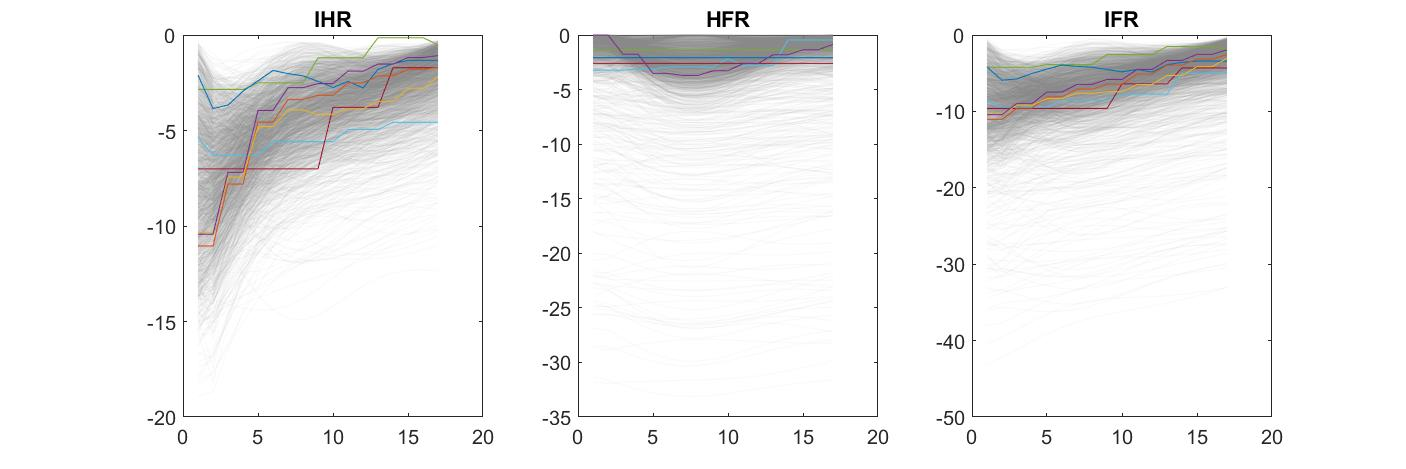
\includegraphics{README_files/figure-gfm/ratesbyage.jpeg}
\caption{\label{fig:ratesbyage} Infection hospitalisation and fatality ratios are generated by modelling profiles from SARS and influenza ratios. x axis: age group index. y axis: log ratio. Colours: seven example profiles. Grey: sampled profiles. Profiles are built from values in Table \ref{tab:pathogenprofile}.}
\end{figure}

\section{Parametric distributions}\label{parametric-distributions}

\begin{longtable}[]{@{}
  >{\centering\arraybackslash}p{(\columnwidth - 8\tabcolsep) * \real{0.3176}}
  >{\centering\arraybackslash}p{(\columnwidth - 8\tabcolsep) * \real{0.1765}}
  >{\centering\arraybackslash}p{(\columnwidth - 8\tabcolsep) * \real{0.1765}}
  >{\centering\arraybackslash}p{(\columnwidth - 8\tabcolsep) * \real{0.1647}}
  >{\centering\arraybackslash}p{(\columnwidth - 8\tabcolsep) * \real{0.1647}}@{}}
\caption{Parameter distributions. \label{tab:paramdist}}\tabularnewline
\toprule\noalign{}
\begin{minipage}[b]{\linewidth}\centering
Parameter
\end{minipage} & \begin{minipage}[b]{\linewidth}\centering
Income group
\end{minipage} & \begin{minipage}[b]{\linewidth}\centering
Distribution
\end{minipage} & \begin{minipage}[b]{\linewidth}\centering
Parameter 1
\end{minipage} & \begin{minipage}[b]{\linewidth}\centering
Parameter 2
\end{minipage} \\
\midrule\noalign{}
\endfirsthead
\toprule\noalign{}
\begin{minipage}[b]{\linewidth}\centering
Parameter
\end{minipage} & \begin{minipage}[b]{\linewidth}\centering
Income group
\end{minipage} & \begin{minipage}[b]{\linewidth}\centering
Distribution
\end{minipage} & \begin{minipage}[b]{\linewidth}\centering
Parameter 1
\end{minipage} & \begin{minipage}[b]{\linewidth}\centering
Parameter 2
\end{minipage} \\
\midrule\noalign{}
\endhead
\bottomrule\noalign{}
\endlastfoot
internet coverage & LLMIC & Beta & 1.78 & 3.11 \\
internet coverage & UMIC & Beta & 14.32 & 6.44 \\
internet coverage & HIC & Beta & 9.57 & 1.39 \\
remaining international
tourism & all & Log normal & -1.39 & 0.39 \\
Labour share of GVA & LLMIC & Beta & 5.09 & 4.51 \\
Labour share of GVA & UMIC & Beta & 7.06 & 8.18 \\
Labour share of GVA & HIC & Beta & 7.97 & 6.87 \\
gdp to gnippp & LLMIC & Gamma & 9.4 & 0.33 \\
gdp to gnippp & UMIC & Gamma & 16.4 & 0.14 \\
gdp to gnippp & HIC & Gamma & 11.89 & 0.12 \\
Hospital capacity & LLMIC & Gamma & 1.3 & 20.2 \\
Hospital capacity & UMIC & Gamma & 1.73 & 40.73 \\
Hospital capacity & HIC & Gamma & 2.05 & 46.57 \\
tourism P1+P2 & all & NA & 6.73 & NA \\
Tourism to international & all & NA & 4.14 & 0.05 \\
pupil teacher ratio & LLMIC & Gamma & 9.15 & 3.11 \\
pupil teacher ratio & UMIC & Gamma & 13.29 & 1.22 \\
pupil teacher ratio & HIC & Gamma & 14.53 & 0.86 \\
school1 fraction & all & Beta & 2.14 & 3.38 \\
school2 fraction & all & Beta & 13.23 & 10.85 \\
work fraction & all & Beta & 10.94 & 13.83 \\
hospitality1 fraction & all & Beta & 21.08 & 381.2 \\
hospitality2 fraction & all & Beta & 3.71 & 88.67 \\
hospitality3 fraction & all & Beta & 19.44 & 149.4 \\
hospitality4 fraction & all & Beta & 7.69 & 62.33 \\
hospitality age1 & all & NA & 0.63 & 0.09 \\
hospitality age2 & all & NA & 0.57 & 0.06 \\
hospitality age3 & all & NA & 0.85 & 0.08 \\
hospitality age4 & all & NA & 0.56 & 0.41 \\
workforce in place & LLMIC & Beta & 3.69 & 2.16 \\
workforce in place & UMIC & Beta & 5.72 & 2.64 \\
workforce in place & HIC & Beta & 9.26 & 2.01 \\
\end{longtable}

\subsection{Hospital capacity}\label{hospital-capacity}

\begin{figure}
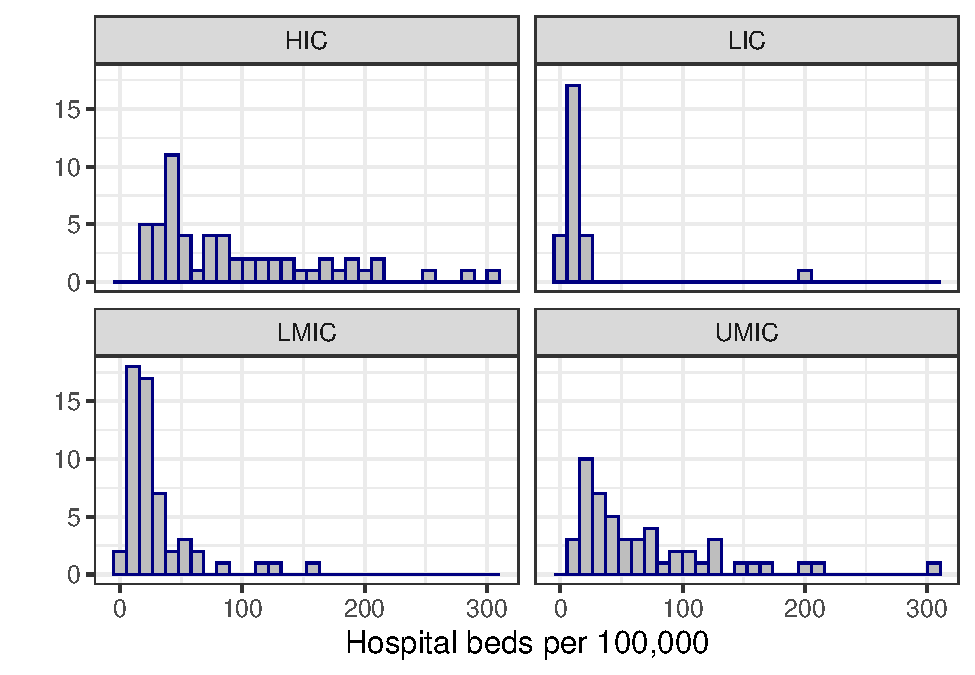
\includegraphics[width=0.5\linewidth]{README_files/figure-latex/hmax-1} \caption{Hospital capacity: available beds minus usual occupancy.}\label{fig:hmax}
\end{figure}

We model these values with gamma distributions. For LLMICs, we have parameters 1.3 and 0.05. For UMICs, we have parameters 1.73 and 0.02. For HICs, we have parameters 2.05 and 0.02. (Data sources: World Bank (beds); OECD, WHO euro (bed occupancy rates).)

\subsection{Labour share of GVA}\label{labour-share-of-gva}

We estimate the average annual income per working-age adult as the total GVA multiplied by the fraction of GVA that goes to labour divided by the number of working-age adults. For the fraction of GVA that goes to labour we use PWT estimates from 2011 (Figure \ref{fig:labsh}).

\begin{figure}
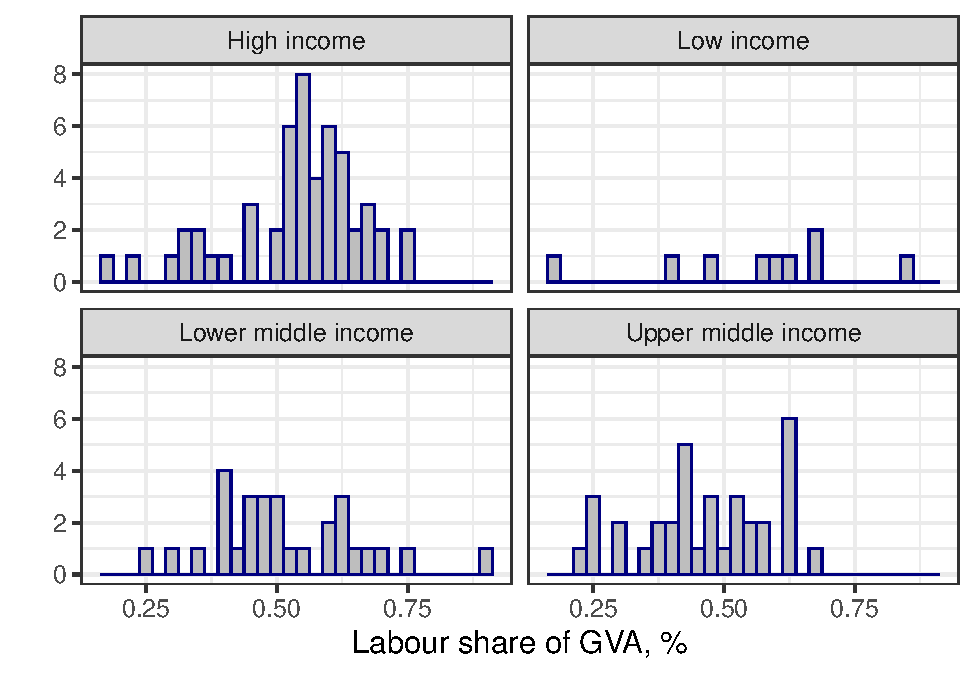
\includegraphics[width=0.5\linewidth]{README_files/figure-latex/labsh-1} \caption{Fraction of GVA that goes to labour (PWT, 2011).}\label{fig:labsh}
\end{figure}

We model these values with Beta distributions. For LLMICs, we have parameters 5.09 and 4.51. For UMICs, we have parameters 7.06 and 8.18. For HICs, we have parameters 7.97 and 6.87.

\subsection{Vaccine administration}\label{vaccine-administration}

\begin{figure}
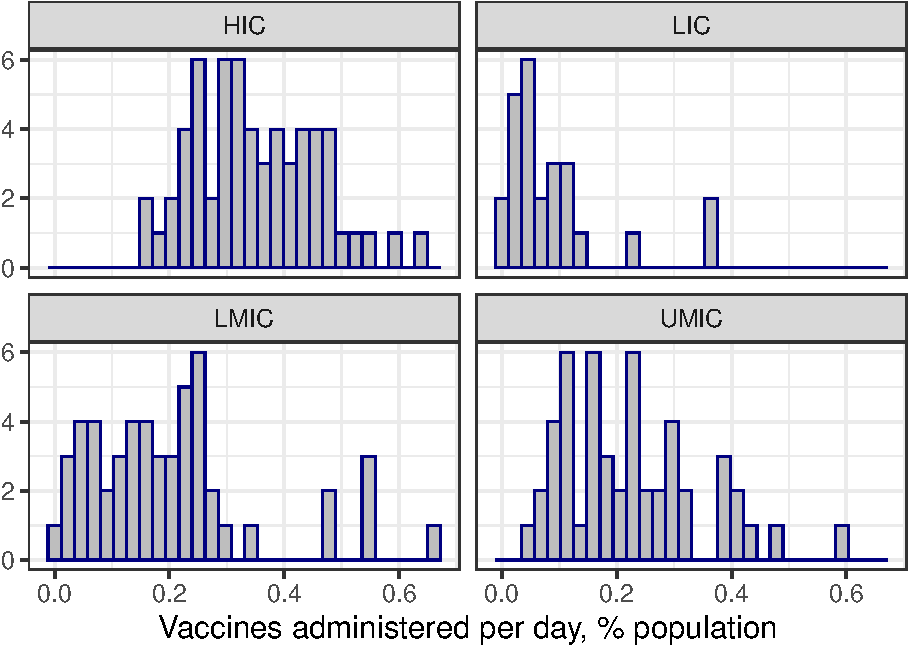
\includegraphics[width=0.5\linewidth]{README_files/figure-latex/vaxrate-1} \caption{Vaccines administered per day, on average, in each country as a percent of population. Data source: fully vaccinated people from OWID (2022).}\label{fig:vaxrate}
\end{figure}

Figure \ref{fig:vaxrate} shows histograms of COVID-19 vaccine administration rates by income level. Values are estimates of administration rates of complete schedules given. Administration rates are estimated as the best-fit slope observed in the pandemic period (Figure \ref{fig:vaxratemx}). The administration slope ideally represents the highest rate possible: rates are often low to begin with, due to limited supply. They are often low at the end, due to depleted demand.

Using the method illustrated in Figure \ref{fig:vaxratemx}, we estimate how many countries per income group surpassed an average maximum rate of 0.5\% of the population per day: 7\% of HICs, 2\% of UMICs, and 5\% of LLMICs.

\begin{figure}
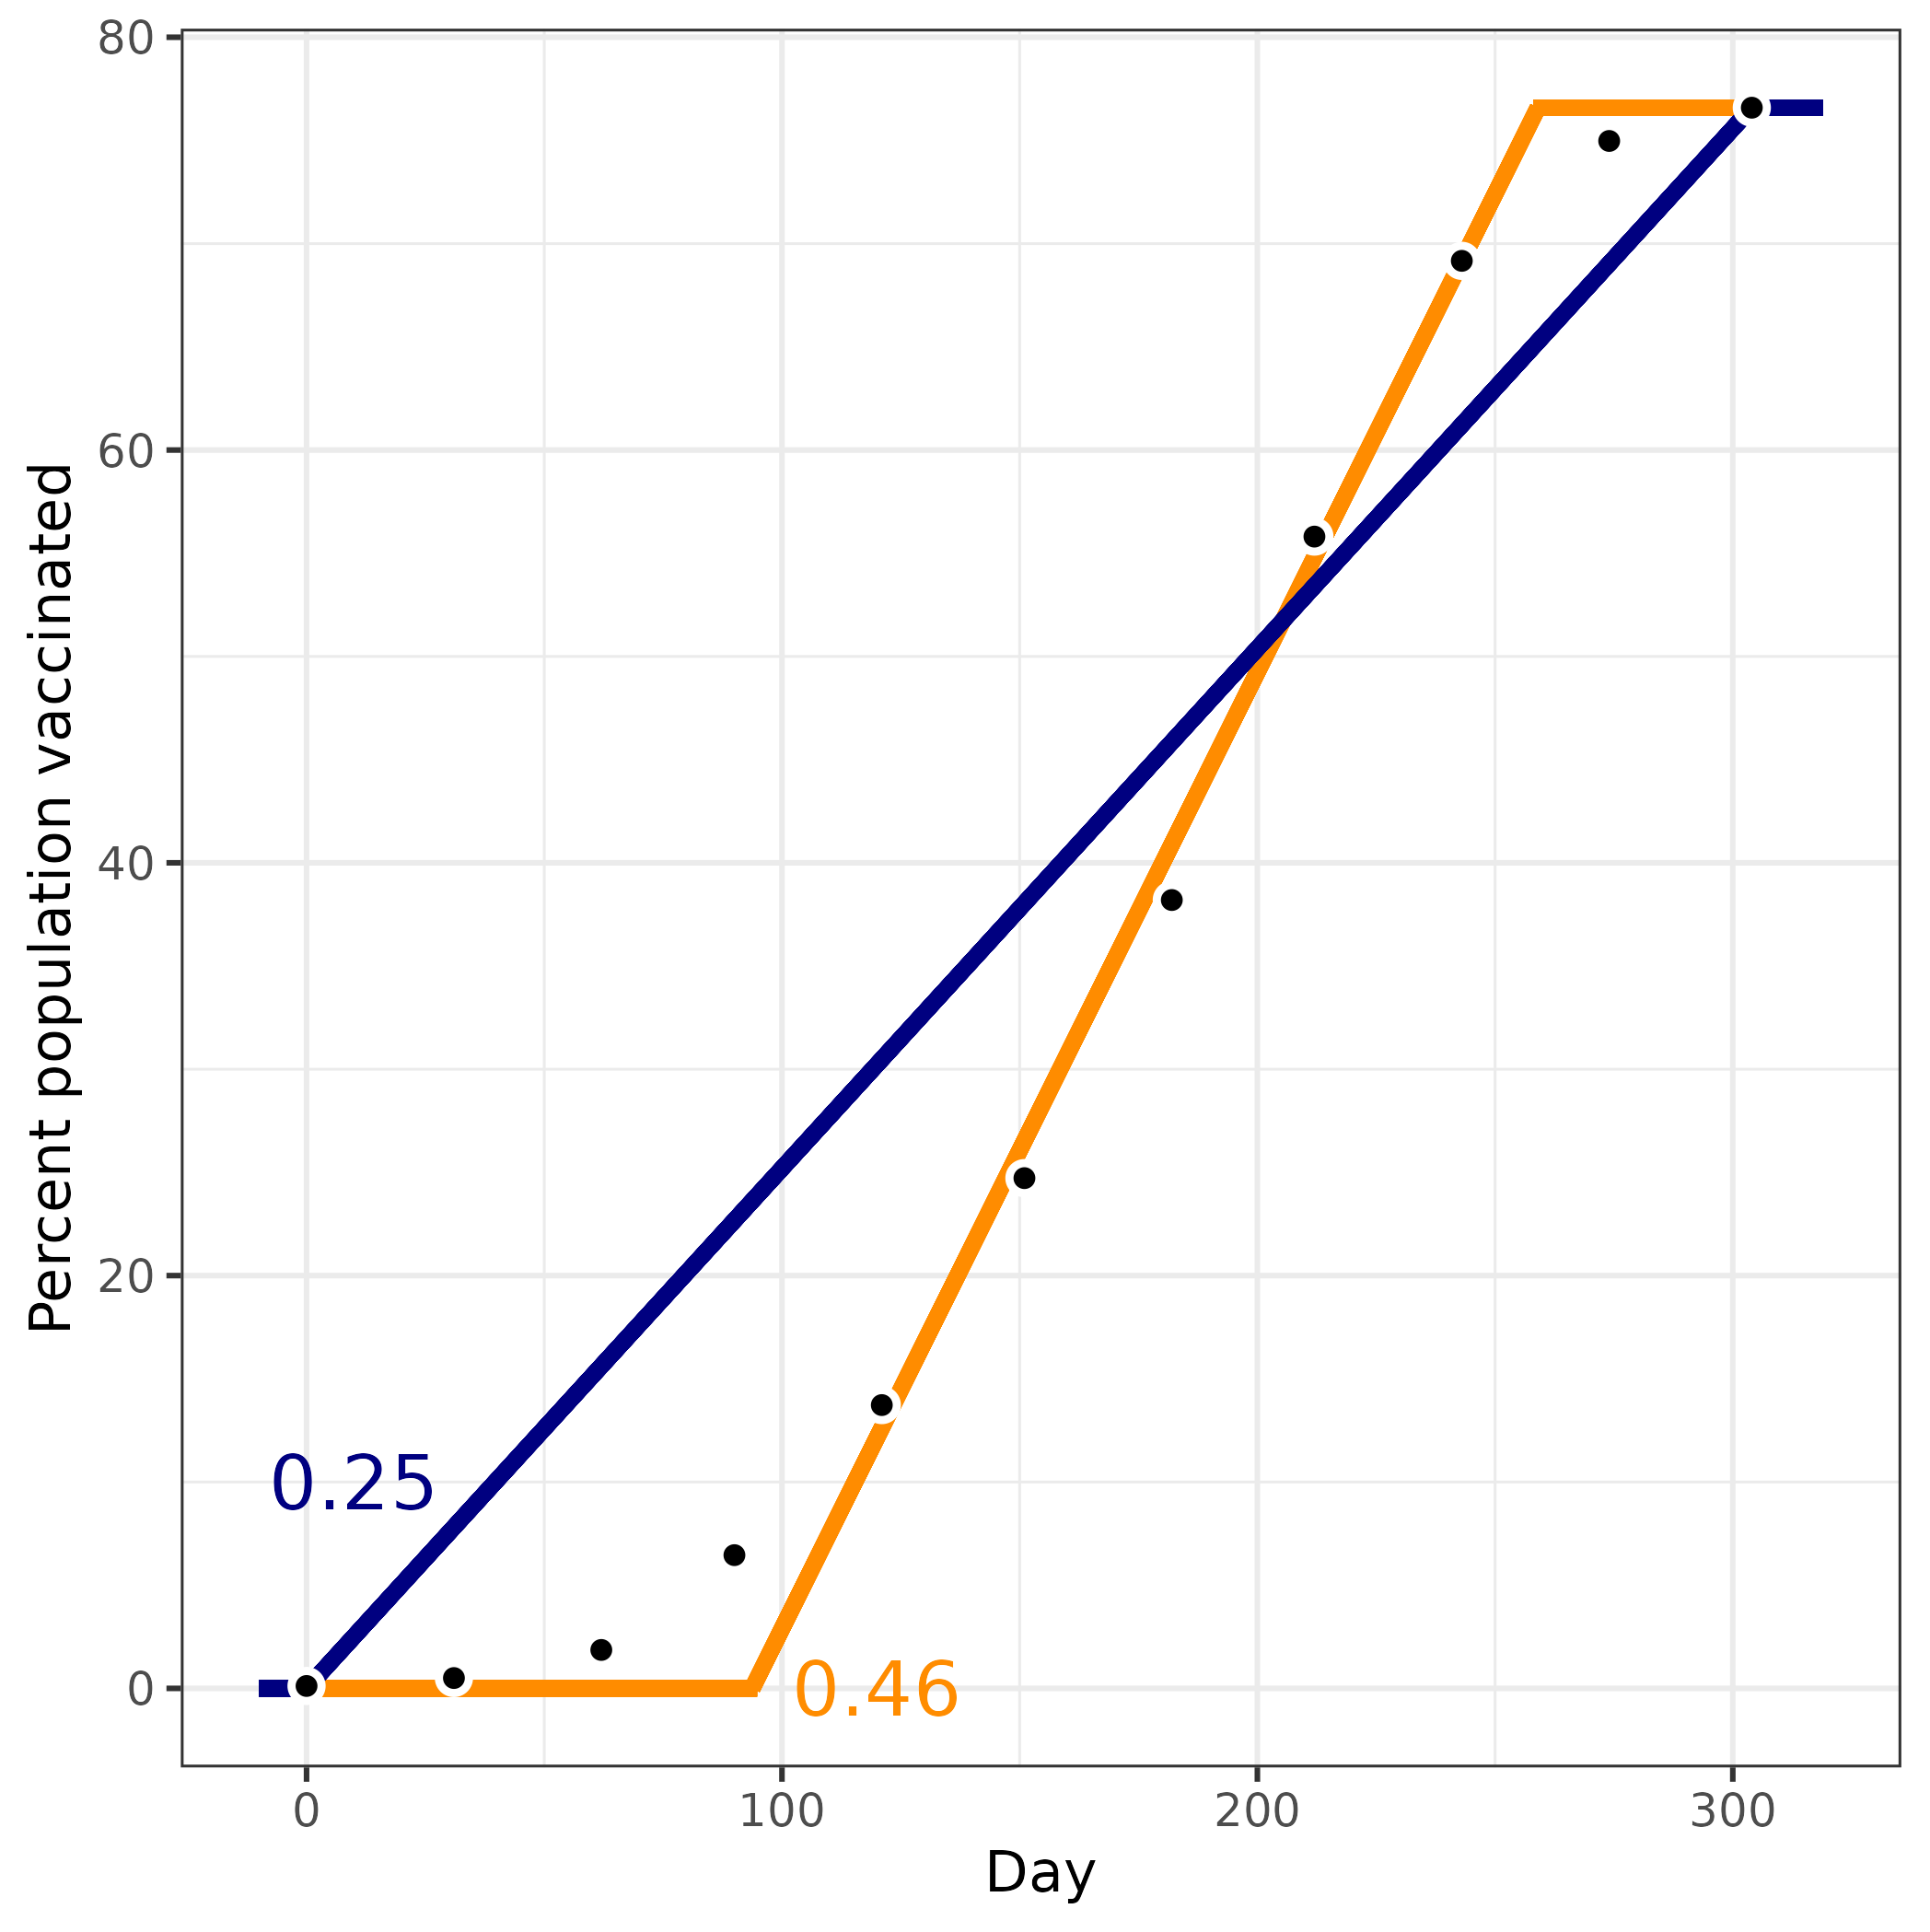
\includegraphics[width=0.5\linewidth]{README_files/figure-gfm/vax_rate_MX} \caption{Vaccine administration in Mexico. The blue line shows the average rate over the whole vaccination campaign. The yellow line shows the average rate when administration was rate limiting.}\label{fig:vaxratemx}
\end{figure}

In LMICs and LICs, there was arguably not a period of vaccine delivery in which the rate was limited by neither demand nor supply. Therefore we use an alternative source to validate our choices of administration rate in different scenarios.

Figure \ref{fig:vaxratewho} shows that in 40\% of vaccination campaigns in LLMICs, the rate exceeded 0.2\% of the population per day; in 28\% of campaigns, the rate exceeded 0.4\% of the population per day; and in 13\% of campaigns, the rate exceeded 1\% of the population per day. We use these rates of delivery for LLMIC synthetic countries.

\begin{figure}
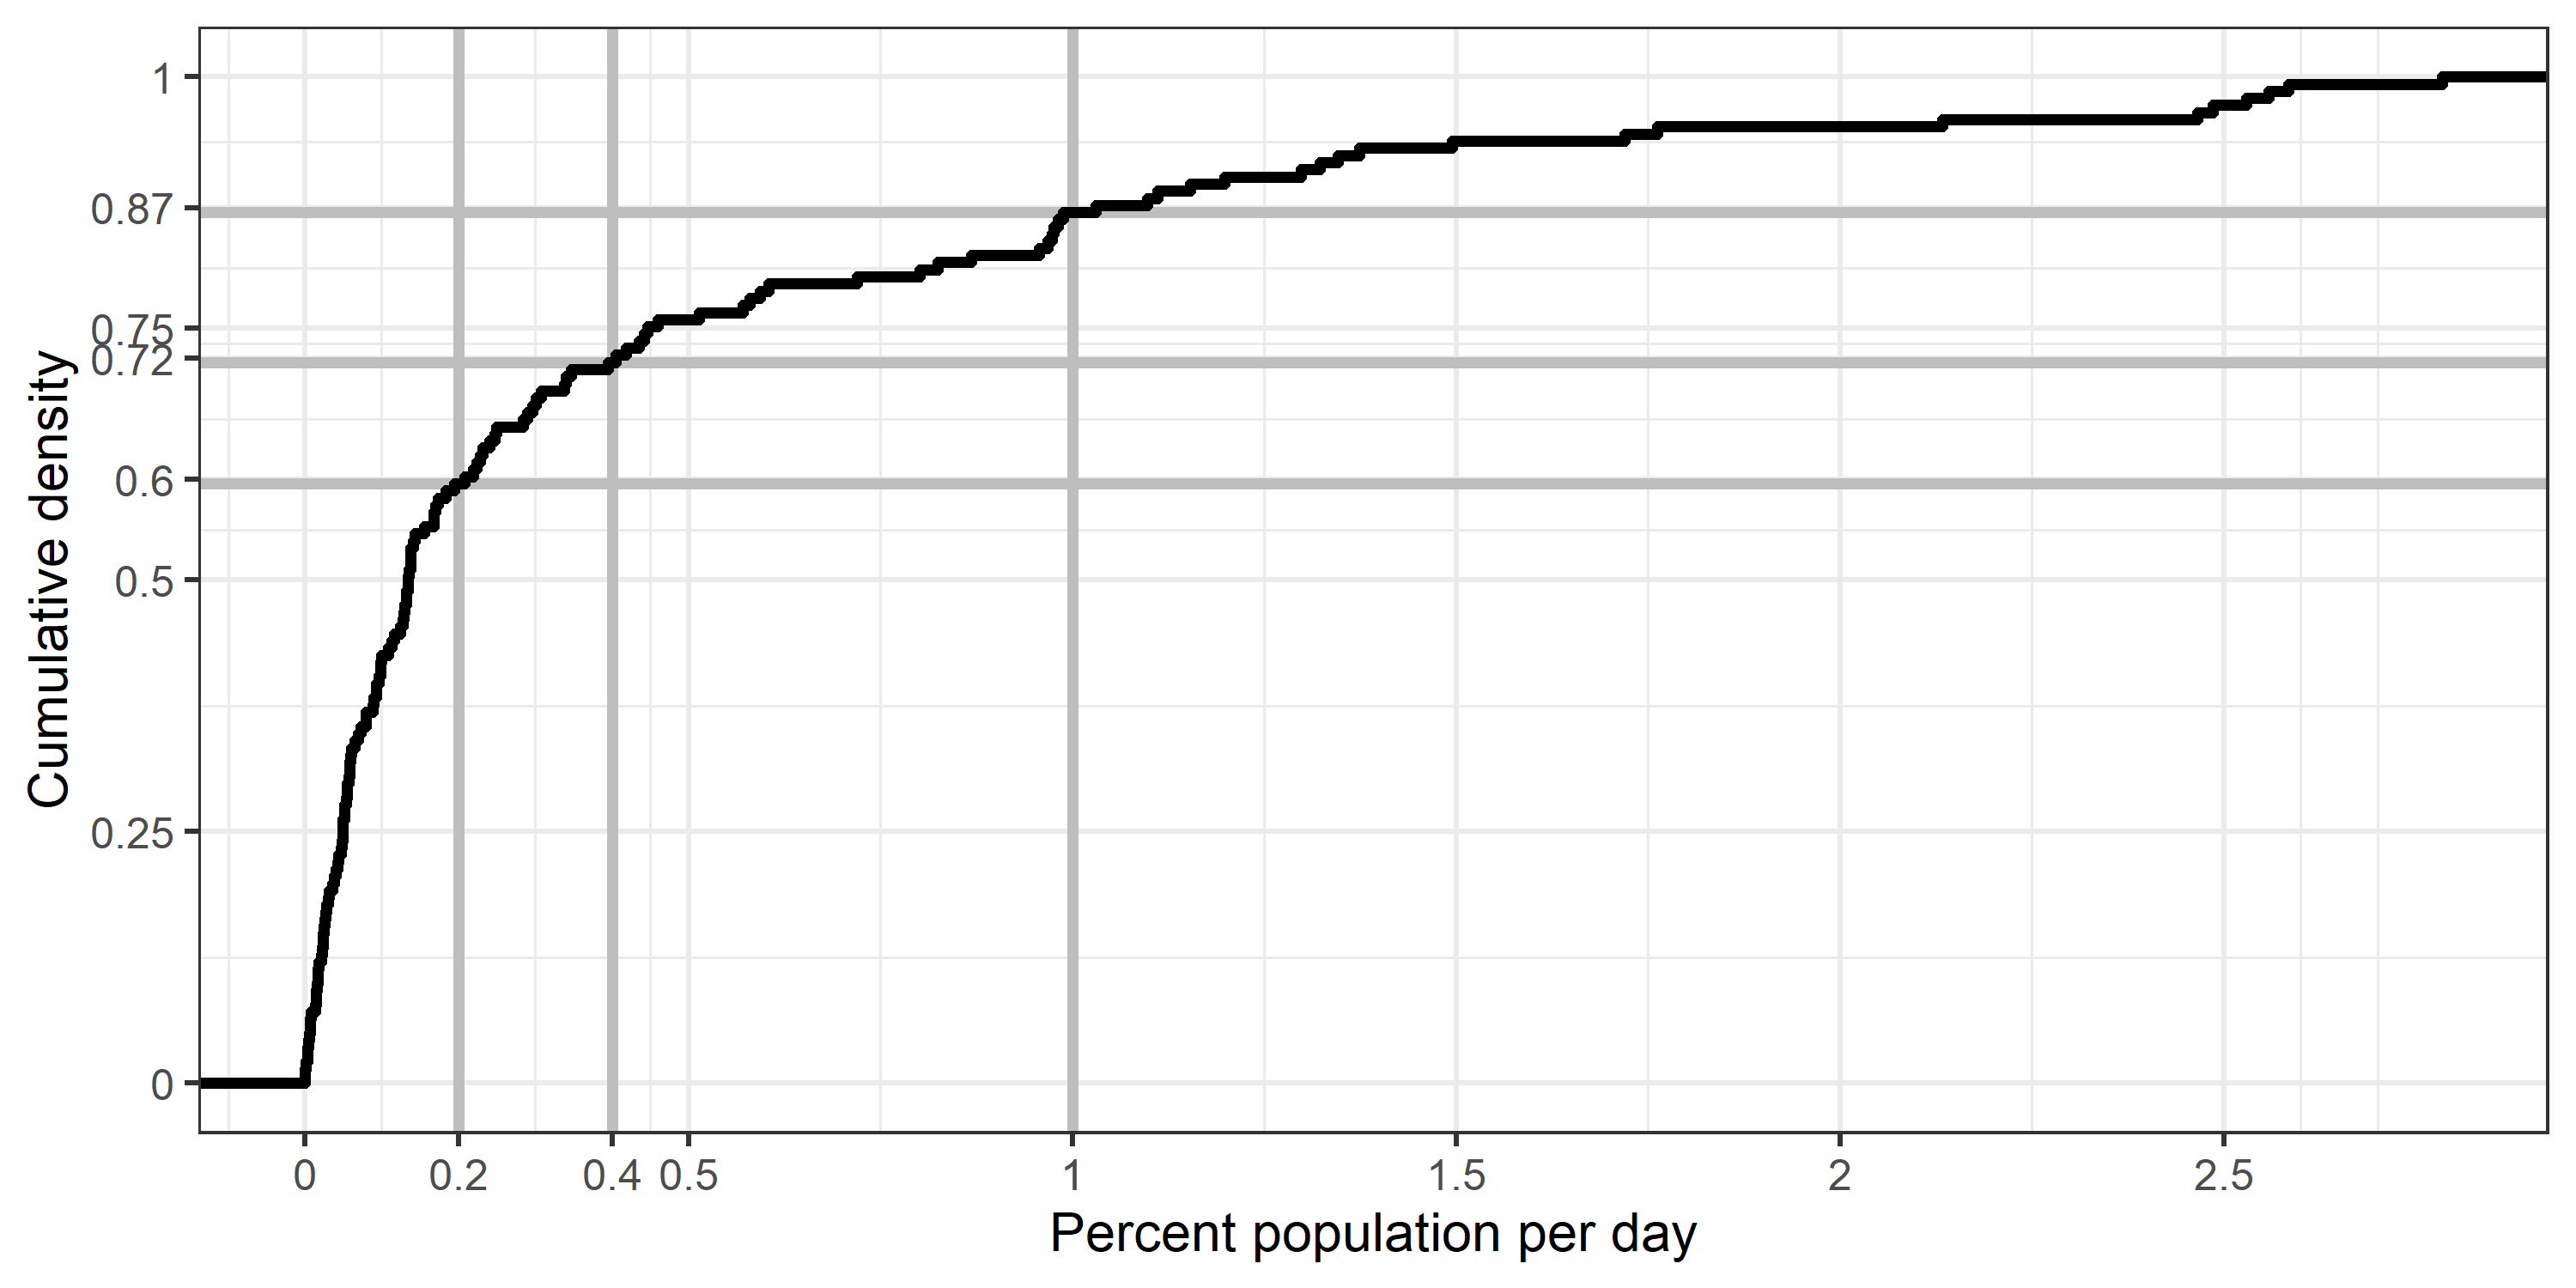
\includegraphics[width=0.8\linewidth]{README_files/figure-gfm/vaccinationrates} \caption{Vaccine administration rates in LLMICs. Shown is the cumulative distribution of delivery rate, measured as the \% of the population vaccinated per day. The data consist of 141 points, from 55 countries that are currently classified as LIC or LMIC, from the years 2000 to 2022, of programmes for measles, MR or MMR vaccines, lasting two weeks or more [@whoSummaryMeaslesRubellaSupplementary2022]. The types of programme include campaigns and outbreak response as well as catch up, follow up, speed up, and mop up.}\label{fig:vaxratewho}
\end{figure}

\subsection{Compliance with the requirement to self isolate}\label{compliance-with-the-requirement-to-self-isolate}

We use a broad Beta distribution with parameters (5,5) to describe the compliance of the population with the requirement to isolate if symptomatic or positive. A YouGov survey \citep{jonessarahpImperialCollegeLondon2020} asked ``If you were advised to do so by a healthcare professional or public health authority to what extent are you willing or not to self-isolate for 7 days?'' The question was asked in 30 different countries (21 high income, five upper-middle income, four lower-middle income) and 63 different weeks of the COVID-19 pandemic to a total of 837,368 people.

The possible answers were `Very unwilling', `Somewhat unwilling', `Neither willing nor unwilling', `Not sure', `Somewhat willing', `Very willing'. Excluding the answer `Not sure', and weighting all other answers on a uniform scale of 0 to 1, the average compliance from all participants is 84\%. The range across countries is 73\% to 90\%. The average value for the UK is 87\%. In contrast, \citet{Smith2021} found that duration-adjusted adherence to full self isolation was 42.5\%. The average value for Australia was 88\%. A survey undertaken in 2009 found that 55\% of households complied with quarantine requirements (\url{https://doi.org/10.1186/1471-2334-11-2}).

\newpage

\section{Notation}\label{notation}

In general in this notation, subscripts are indices, and superscripts are never indices but instead define new labels. In particular, note that numerical superscripts are attached to letters \(k\) for rates and \(p\) for parameters. Where a power is applied to one of these letters, the letter will be enclosed in parentheses for clarity.

\begin{longtable}[]{@{}
  >{\centering\arraybackslash}p{(\columnwidth - 6\tabcolsep) * \real{0.1980}}
  >{\centering\arraybackslash}p{(\columnwidth - 6\tabcolsep) * \real{0.3267}}
  >{\centering\arraybackslash}p{(\columnwidth - 6\tabcolsep) * \real{0.1584}}
  >{\centering\arraybackslash}p{(\columnwidth - 6\tabcolsep) * \real{0.3168}}@{}}
\caption{Capital letters}\tabularnewline
\toprule\noalign{}
\begin{minipage}[b]{\linewidth}\centering
Letter
\end{minipage} & \begin{minipage}[b]{\linewidth}\centering
Script
\end{minipage} & \begin{minipage}[b]{\linewidth}\centering
Subscript
\end{minipage} & \begin{minipage}[b]{\linewidth}\centering
Superscript
\end{minipage} \\
\midrule\noalign{}
\endfirsthead
\toprule\noalign{}
\begin{minipage}[b]{\linewidth}\centering
Letter
\end{minipage} & \begin{minipage}[b]{\linewidth}\centering
Script
\end{minipage} & \begin{minipage}[b]{\linewidth}\centering
Subscript
\end{minipage} & \begin{minipage}[b]{\linewidth}\centering
Superscript
\end{minipage} \\
\midrule\noalign{}
\endhead
\bottomrule\noalign{}
\endlastfoot
\(A\) & & & \\
\(B\) & & & \\
\(C\) & consumption & & community (contacts) \\
\(D\) & COMPARTMENT: Died & & related to death state \\
\(E\) & COMPARTMENT: Exposed & & related to exposed state \\
\(F\) & & & \\
\(G\) & & & \\
\(GDP\) & GDP & & \\
\(H\) & COMPARTMENT: Hospitalised & & related to hospitalised state \\
\(H_{\text{max}}\) & hospital capacity & & \\
\(I\) & Infectious & & \\
\(I^{a}\) & COMPARTMENT: Infectious
asymptomatic & & related to asymptomatic state \\
\(I^{s}\) & COMPARTMENT: Infectious
symptomatic & & related to symptomatic state \\
\(J\) & & MAX: strata & \\
\(K\) & Loss (cost calculation) & & \\
\(L\) & number of people by sector
(workforce in place) & & \\
\(M^{\text{com}}\) & CONTACTS: community & & \\
\(M^{\text{home}}\) & CONTACTS: community, home & & \\
\(M^{\text{CC}}\) & CONTACTS: community, customers & & \\
\(M^{\text{trav}}\) & CONTACTS: community, public
transport & & \\
\(M^{\text{sch}}\) & CONTACTS: community, school & & \\
\(M^{\text{WC}}\) & CONTACTS: work, worker to
customer & & \\
\(M^{\text{CW}}\) & CONTACTS: work, customer to
worker & & \\
\(M\) & CONTACTS: total & & \\
\(\tilde{M}\) & Total contacts by five-year
age bands & & \\
\(\hat{M}\) & Total contacts by DAEDALUS age
groups & & \\
\(N\) & number of people by stratum & & \\
\(\tilde{N}\) & Number of people by five-year
age bands & & \\
\(\hat{N}\) & Number of people in DAEDALUS
age groups & & \\
\(O\) & -- & & \\
\(P\) & (probability) & & \\
\(Q\) & & & \\
\(R\) & COMPARTMENT: Recovered & & related to recovered state \\
\(R_0\) & Basic reproduction number & & \\
\(R_t\) & Effective reproduction number & & \\
\(S\) & COMPARTMENT: Susceptible & MAX: sectors & \\
\(S^{c}\) & COMPARTMENT: Susceptible
seroconverting & & \\
\(T^c\) & duration from vaccination to
protection & & \\
\(T^H\) & duration in hospital & & \\
\(T^{H:D}\) & duration in hospital given
death & & \\
\(T^{H:R}\) & duration in hospital given
recovery & & \\
\(T^{I^a}\) & duration asymptomatic & & \\
\(T^{I^s}\) & duration symptomatic & & \\
\(T^{I^s:H}\) & duration symptomatic given
hospitalised & & \\
\(T^{I^s:R}\) & duration symptomatic given
recovery & & \\
\(T^{E:I}\) & latent period & & \\
\(U\) & & & \\
\(V\) & & MAX: vaccines & \\
\(W\) & & & worker (contacts) \\
\(X\) & & & \\
\(Y\) & GDP & MAX: years & \\
\(Y_0\) & max GDP & & \\
\(Z\) & & & \\
\end{longtable}

\begin{longtable}[]{@{}
  >{\centering\arraybackslash}p{(\columnwidth - 6\tabcolsep) * \real{0.1782}}
  >{\centering\arraybackslash}p{(\columnwidth - 6\tabcolsep) * \real{0.3267}}
  >{\centering\arraybackslash}p{(\columnwidth - 6\tabcolsep) * \real{0.3267}}
  >{\centering\arraybackslash}p{(\columnwidth - 6\tabcolsep) * \real{0.1683}}@{}}
\caption{Lower-case letters}\tabularnewline
\toprule\noalign{}
\begin{minipage}[b]{\linewidth}\centering
Letter
\end{minipage} & \begin{minipage}[b]{\linewidth}\centering
Script
\end{minipage} & \begin{minipage}[b]{\linewidth}\centering
Subscript
\end{minipage} & \begin{minipage}[b]{\linewidth}\centering
Superscript
\end{minipage} \\
\midrule\noalign{}
\endfirsthead
\toprule\noalign{}
\begin{minipage}[b]{\linewidth}\centering
Letter
\end{minipage} & \begin{minipage}[b]{\linewidth}\centering
Script
\end{minipage} & \begin{minipage}[b]{\linewidth}\centering
Subscript
\end{minipage} & \begin{minipage}[b]{\linewidth}\centering
Superscript
\end{minipage} \\
\midrule\noalign{}
\endhead
\bottomrule\noalign{}
\endlastfoot
\(a\) & & INDEX: age index, five-year
age bands & asymptomatic \\
\(b\) & proportion of tourism that is
international & & \\
\(c\) & fraction international tourism
reduces to as a consequence of
the pandemic & & seroconverting \\
\(d\) & deaths per million & & \\
\(e\) & government mandate & & \\
\(\text{ed}\) & & education sector (j index) & \\
\(f\) & functions: UTR,
hospitalisation & & \\
\(g\) & & INDEX: age index, DAEDALUS age
groups & \\
\(h\) & & INDEX: dummy index & \\
\(i\) & & & self isolating \\
\(j\) & & INDEX: stratum index & \\
\(k\) & state transition rates & & \\
\(l\) & life expectancy & & \\
\(m_J\) & number of strata & & \\
\(m_S\) & number of sectors & & \\
\(m_V\) & number of vaccines & & \\
\(m_Y\) & number of years in work & & \\
\(n\) & & & \\
\(o\) & -- & & \\
\(p\) & parameters & & \\
\(q\) & proportions working from home & & \\
\(r\) & discount rate & & \\
\(s\) & & & symptomatic \\
\(\text{school}\) & & student strata (j index) & \\
\(t\) & time (day) & & \\
\(u\) & dummy variable & INDEX: dummy index & \\
\(v\) & & INDEX: vaccination status & \\
\(w\) & & & \\
\(x\) & sector openness & & \\
\(y\) & GVA & INDEX: year & \\
\(z\) & fraction of GDP coming from
the Food and accommodation
sector & & \\
\end{longtable}

\begin{longtable}[]{@{}
  >{\centering\arraybackslash}p{(\columnwidth - 2\tabcolsep) * \real{0.1806}}
  >{\centering\arraybackslash}p{(\columnwidth - 2\tabcolsep) * \real{0.3611}}@{}}
\caption{Greek letters}\tabularnewline
\toprule\noalign{}
\begin{minipage}[b]{\linewidth}\centering
Letter
\end{minipage} & \begin{minipage}[b]{\linewidth}\centering
Definition
\end{minipage} \\
\midrule\noalign{}
\endfirsthead
\toprule\noalign{}
\begin{minipage}[b]{\linewidth}\centering
Letter
\end{minipage} & \begin{minipage}[b]{\linewidth}\centering
Definition
\end{minipage} \\
\midrule\noalign{}
\endhead
\bottomrule\noalign{}
\endlastfoot
\(\alpha\) & \\
\(\beta\) & transmission rate \\
\(\gamma\) & \\
\(\delta\) & \\
\(\epsilon\) & ratio transmission from
asymptomatic \\
\(\zeta\) & \\
\(\eta\) & vaccine effects \\
\(\theta\) & \\
\(\iota\) & \\
\(\kappa\) & \\
\(\lambda\) & \\
\(\mu\) & \\
\(\nu\) & growth rate \\
\(o\) & -- \\
\(\pi\) & \\
\(\rho\) & transmission modifier \\
\(\sigma\) & \\
\(\tau\) & max time \\
\(\upsilon\) & -- \\
\(\phi\) & \\
\(\chi\) & \\
\(\psi\) & \\
\(\omega\) & \\
\end{longtable}

\begin{longtable}[]{@{}
  >{\centering\arraybackslash}p{(\columnwidth - 2\tabcolsep) * \real{0.1528}}
  >{\centering\arraybackslash}p{(\columnwidth - 2\tabcolsep) * \real{0.4583}}@{}}
\caption{Rates}\tabularnewline
\toprule\noalign{}
\begin{minipage}[b]{\linewidth}\centering
Letter
\end{minipage} & \begin{minipage}[b]{\linewidth}\centering
Definition
\end{minipage} \\
\midrule\noalign{}
\endfirsthead
\toprule\noalign{}
\begin{minipage}[b]{\linewidth}\centering
Letter
\end{minipage} & \begin{minipage}[b]{\linewidth}\centering
Definition
\end{minipage} \\
\midrule\noalign{}
\endhead
\bottomrule\noalign{}
\endlastfoot
\(k^1\) & rate of infection \\
\(k^2\) & rate of onset of asymptomatic
infection \\
\(k^3\) & rate of recovery from
asymptomatic infection \\
\(k^4\) & rate of onset of symptomatic
infection \\
\(k^5\) & rate of recovery from
symptomatic infection \\
\(k^6\) & rate of hospitalisation \\
\(k^7\) & rate of recovery from
hospitalisation \\
\(k^8\) & rate of death from
hospitalisation \\
\(k^9\) & rate of vaccine seroconversion \\
\(k^{10}\) & vaccination rate \\
\(k^{11}\) & \\
\(k^{12}\) & rate of infection \\
\(k^{13}\) & \\
\(k^{14}\) & \\
\(k^{15}\) & \\
\(k^{16}\) & \\
\(k^{17}\) & \\
\(k^{18}\) & \\
\(k^{19}\) & rate of infection \\
\end{longtable}

\begin{longtable}[]{@{}
  >{\centering\arraybackslash}p{(\columnwidth - 2\tabcolsep) * \real{0.2222}}
  >{\centering\arraybackslash}p{(\columnwidth - 2\tabcolsep) * \real{0.4583}}@{}}
\caption{Parameters}\tabularnewline
\toprule\noalign{}
\begin{minipage}[b]{\linewidth}\centering
Letter
\end{minipage} & \begin{minipage}[b]{\linewidth}\centering
Definition
\end{minipage} \\
\midrule\noalign{}
\endfirsthead
\toprule\noalign{}
\begin{minipage}[b]{\linewidth}\centering
Letter
\end{minipage} & \begin{minipage}[b]{\linewidth}\centering
Definition
\end{minipage} \\
\midrule\noalign{}
\endhead
\bottomrule\noalign{}
\endlastfoot
\(p^{I^S}\) & probability to be symptomatic \\
\(\tilde{p}^H\) & Basic probability to be
hospitalised \\
\(p^H\) & Adjusted probability to be
hospitalised \\
\(\tilde{p}^D\) & Basic probability to die \\
\(p^D\) & Adjusted probability to die \\
\(p^1\) & Compliance with the
instruction to self isolate \\
\(p^2\) & fraction of cases identified
by testing \\
\(p^3\) & proportion of asymptomatic
infectiousness averted due to
self isolating \\
\(p^4\) & proportion of symptomatic
infectiousness averted due to
self isolating \\
\(p^5\) & tourism parameter \\
\(p^6\) & tourism parameter \\
\(p^7\) & tourism parameter \\
\(p^8\) & minimum mobility \\
\(p^9\) & deaths coefficient for
mobility \\
\(p^{10}\) & mandate coefficient for
mobility \\
\(p^{11}\) & mobility mixing parameter \\
\(p^{12}\) & present value of lost earnings \\
\(p^{13}\) & mean annual earnings \\
\(p^{14}\) & effective amount of education
lost per student \\
\(p^{15}\) & rate of return for one year of
education \\
\(p^{16}\) & relative effectiveness of
remote education \\
\(p^{17}\) & number of days from onset of
infectiousness to self
isolation \\
\(p^{18}\) & number of asymptomatic days
spent in self isolation per
day of infectiousness \\
\(p^{19}\) & number of symptomatic days
spent in self isolation per
day of infectiousness \\
\(p^{20}\) & number of days from onset of
symptoms to self isolation \\
\(p^{21}\) & public transport mode share \\
\(p^{22}\) & work absence, asymptomatic
(cost calculation) \\
\(p^{23}\) & work absence, symptomatic
(cost calculation) \\
\(p^{24}\) & school absence, asymptomatic
(cost calculation) \\
\(p^{25}\) & school absence, symptomatic
(cost calculation) \\
\(p^{26}\) & fraction of symptomatic
infectiousness that is
presymptomatic \\
\(p^{27}\) & hospitality openness \\
\end{longtable}

\newpage

  \bibliography{DAEDALUS.bib}

\end{document}
